\chapter{Methods and Results}

\section{Evaluation of Proposed Speech Intelligibility Prediction Method for Reverberation}

\subsection{Proposed Method}

The goal outlined in this thesis was to analyze the perceptual impacts of reverberation for hearing aid users, and evaluate the perceptual benefit of applying delay-and-predict dereverberation (i.e., DAP dereverberation, Section \ref{section_dap}) to remove reverberant effect. It was intended to perform an evaluation of realistic and practical conditions, and use performance metrics that reflect realistic perceptual impacts with and without hearing loss. 

As described in Section \ref{section_perception}, perception is commonly characterized by speech intelligibility (SI), listening effort (LE) and speech quality (SQ). To accurately evaluate the perceptual impacts of reverberation, a perceptually accurate predictor of SI is needed, which will also correlate implicitly to LE. Among the objective predictors of SI described in Section \ref{section_si_metrics}, the MR NSIM, FT NSIM and STMI were selected since they provide the most physiologically accurate model of the auditory system and the impacts of hearing loss. Although HASPI incorporates a more simplisitic model the auditory system and hearing loss, it is standard in the hearing aid industry and therefore was included to provide a data that could be easily understood by researchers in the field. Lastly STOI, which includes no explicit modeling of the auditory system or hearing loss, was included as because of its standardization accross the entire speech processing industry. Since these are all monaural predictors, an equalization-cancellation (EC) front-end was included to provide some modeling of binaural perceptual benefits (i.e., spatial release from masking, \ref{section_srm}). Recall, however, that the EC algorithm is simplistic and provides no modeling of degredations due to hearing loss.

\textbf{this is the PROPOSED method, modified after analysis of components below}.

For each SI predictor, the impacts of reverberation and benefit of DAP dereverberation were analyzed as follows:

...



\subsection{Analysis of RIR Databases}




\begin{figure}[H]
	\includegraphics[width=1\textwidth]{RIR_EDC_Office}
	\centering
	\caption{HRIR database office II room}
	\label{fig:RIR_EDC_Office}
\end{figure}

•	Listed as 300 msec in paper

•	Measured as approx 

o	T60 = 420 – 7 = 413 msec

o	T30 = 2*(225-25) = 400 msec 



\begin{figure}[H]
	\includegraphics[width=1\textwidth]{RIR_EDC_Courtyard}
	\centering
	\caption{HRIR database courtyard room}
	\label{fig:RIR_EDC_Courtyard}
\end{figure}

•	Listed as 900 msec in paper

•	Measured as approx. 

o	T60 = 430 – 4 = 426 msec

o	T30 = 2*(200-5) = 390 msec


\begin{figure}[H]
	\includegraphics[width=1\textwidth]{RIR_EDC_Cafeteria}
	\centering
	\caption{HRIR database cafeteria room}
	\label{fig:RIR_EDC_Cafeteria}
\end{figure}

•	Listed as 1.25 sec in paper

•	Measured as approx. 

o	T60 = 440 – 3 = 437 msec

o	T30 = 2*(275 – 4) = 542 msec


\begin{figure}[H]
	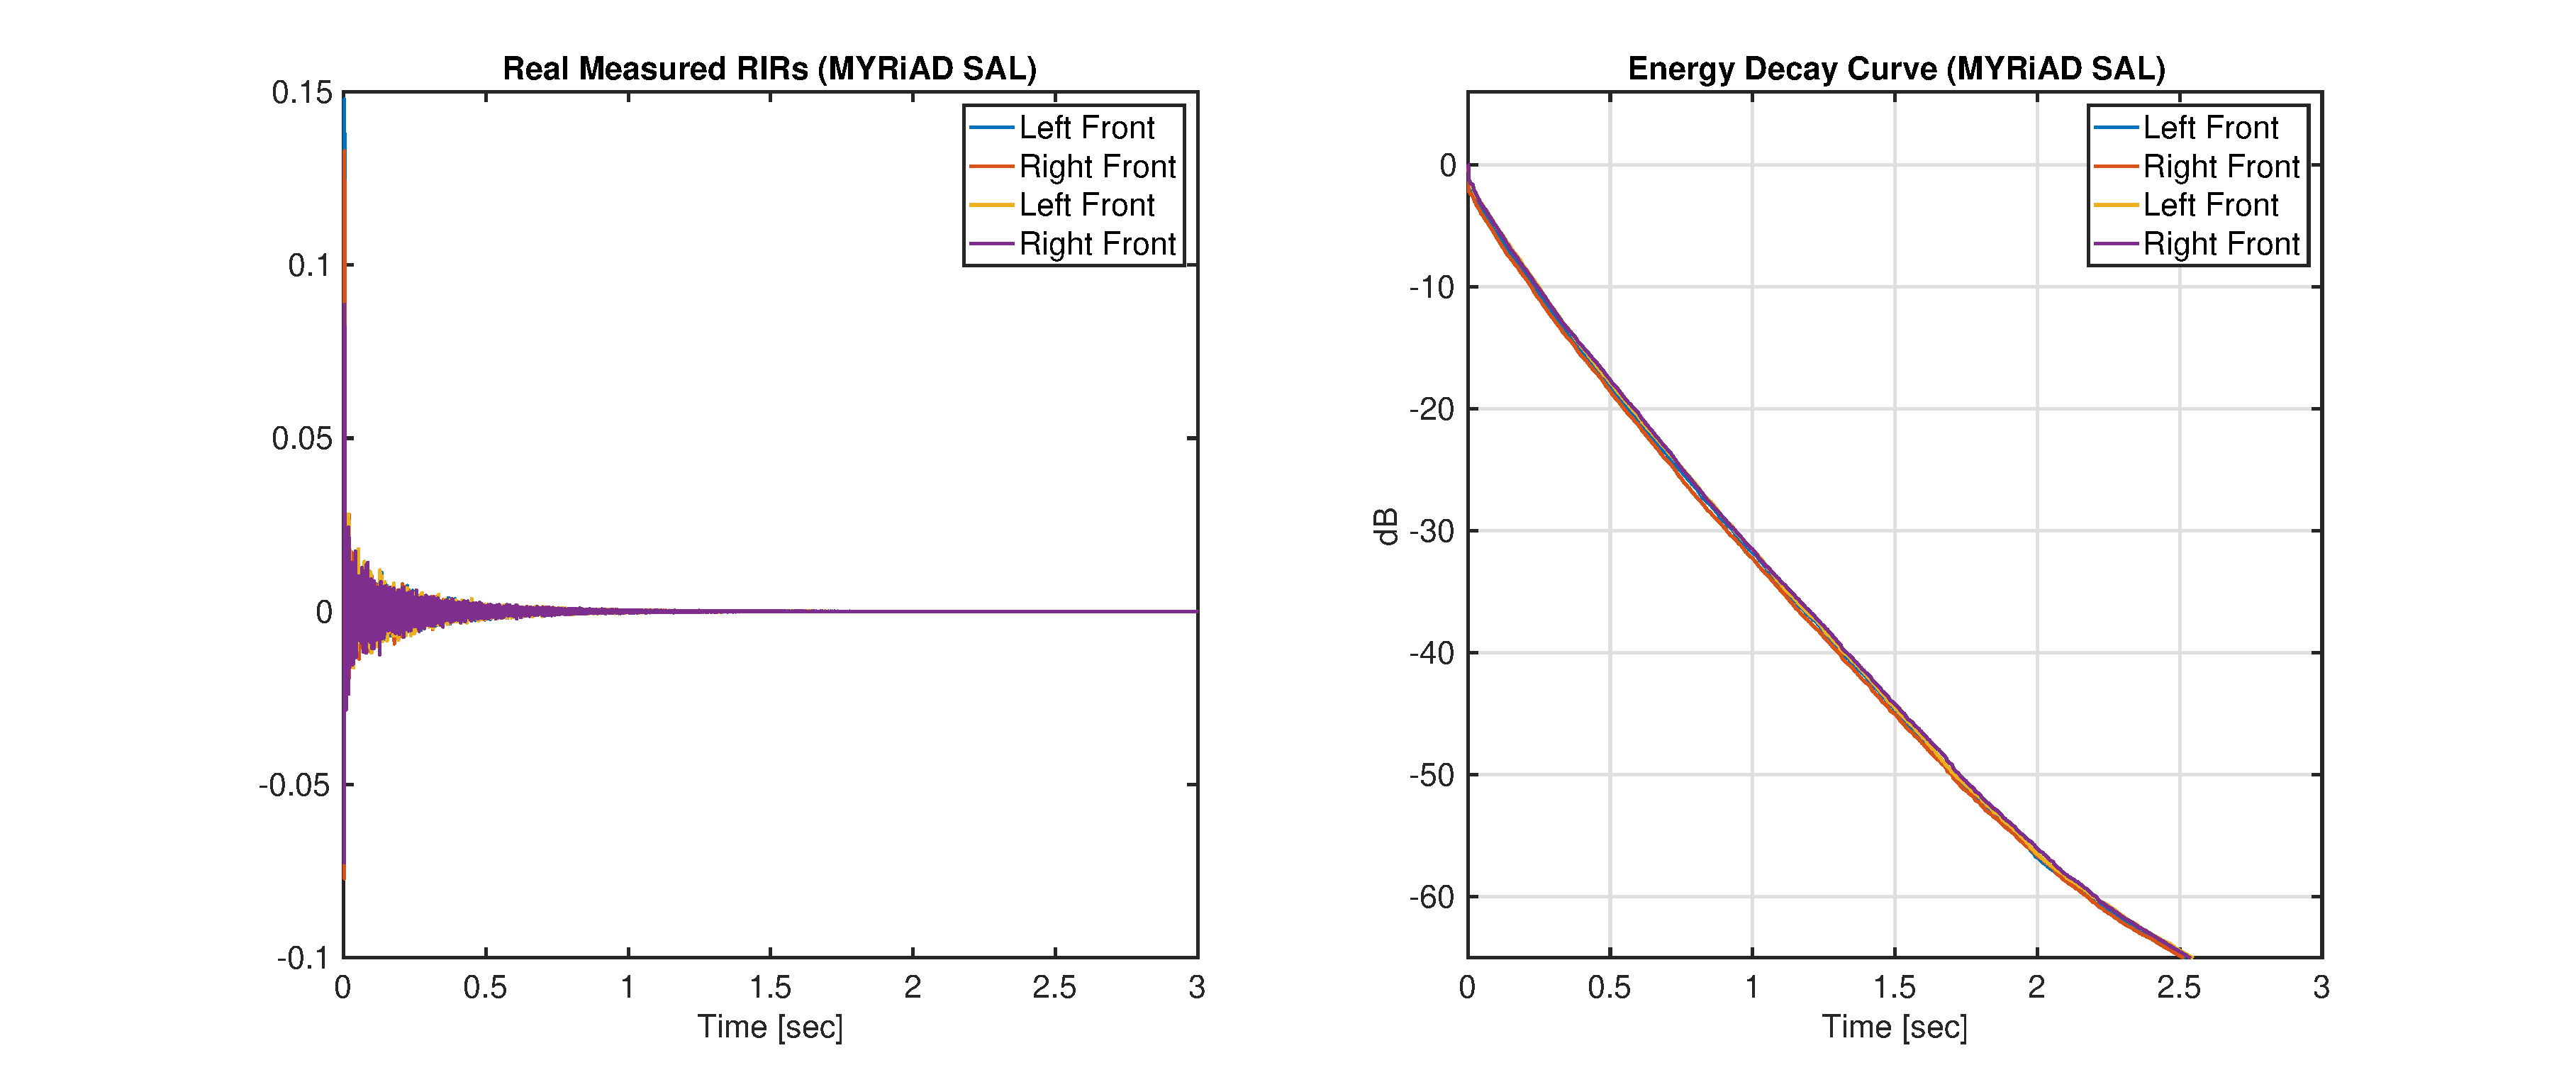
\includegraphics[width=1\textwidth]{RIR_EDC_SAL}
	\centering
	\caption{MYRiAD database SAL room}
	\label{fig:RIR_EDC_SAL}
\end{figure}

•	Listed as 2.1 sec (2100 msec) in paper

•	Measured as approx..

o	T60 = 2200 msec

o	T30 = 2*(1159-100) = 2118 msec


Discuss:

- Add early decay time (EDT) to  chapter 1

- How T60s were calculated in the papers compared to true T60s I'm citing

- EDT of each

- Noise data available also in HRIR (and MYRiAD?)

\subsection{Evaluation of Equalization-Cancellation Front-End}

\textbf{SRM}

\begin{figure}[H]
	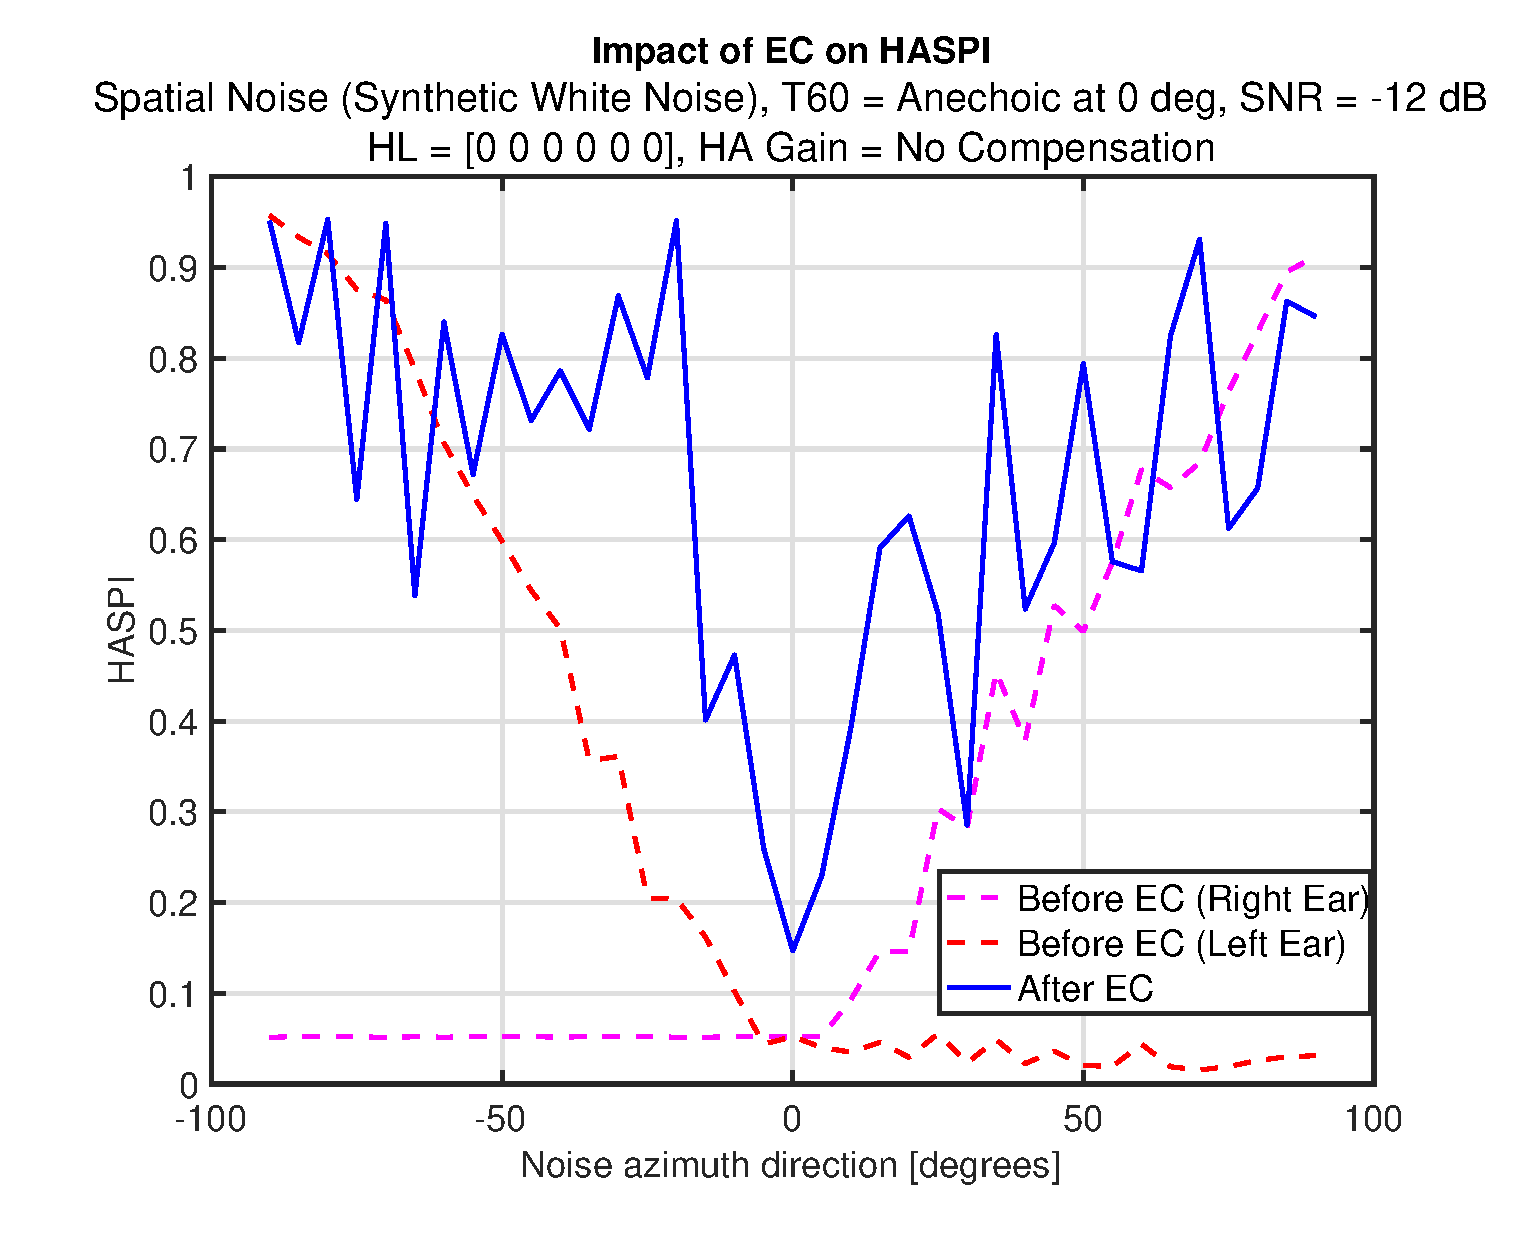
\includegraphics[width=0.7\textwidth]{EC_SRM_NoiseDir}
	\centering
	\caption{Impact of EC algorithm on speech intelligibility (using HASPI) as a function of noise direction, anechoic directional speech and noise}
	\label{fig:EC_SRM_NoiseDir}
\end{figure}

\begin{figure}[H]
	\centering
	\begin{subfigure}[b]{0.49\textwidth}
		\centering
		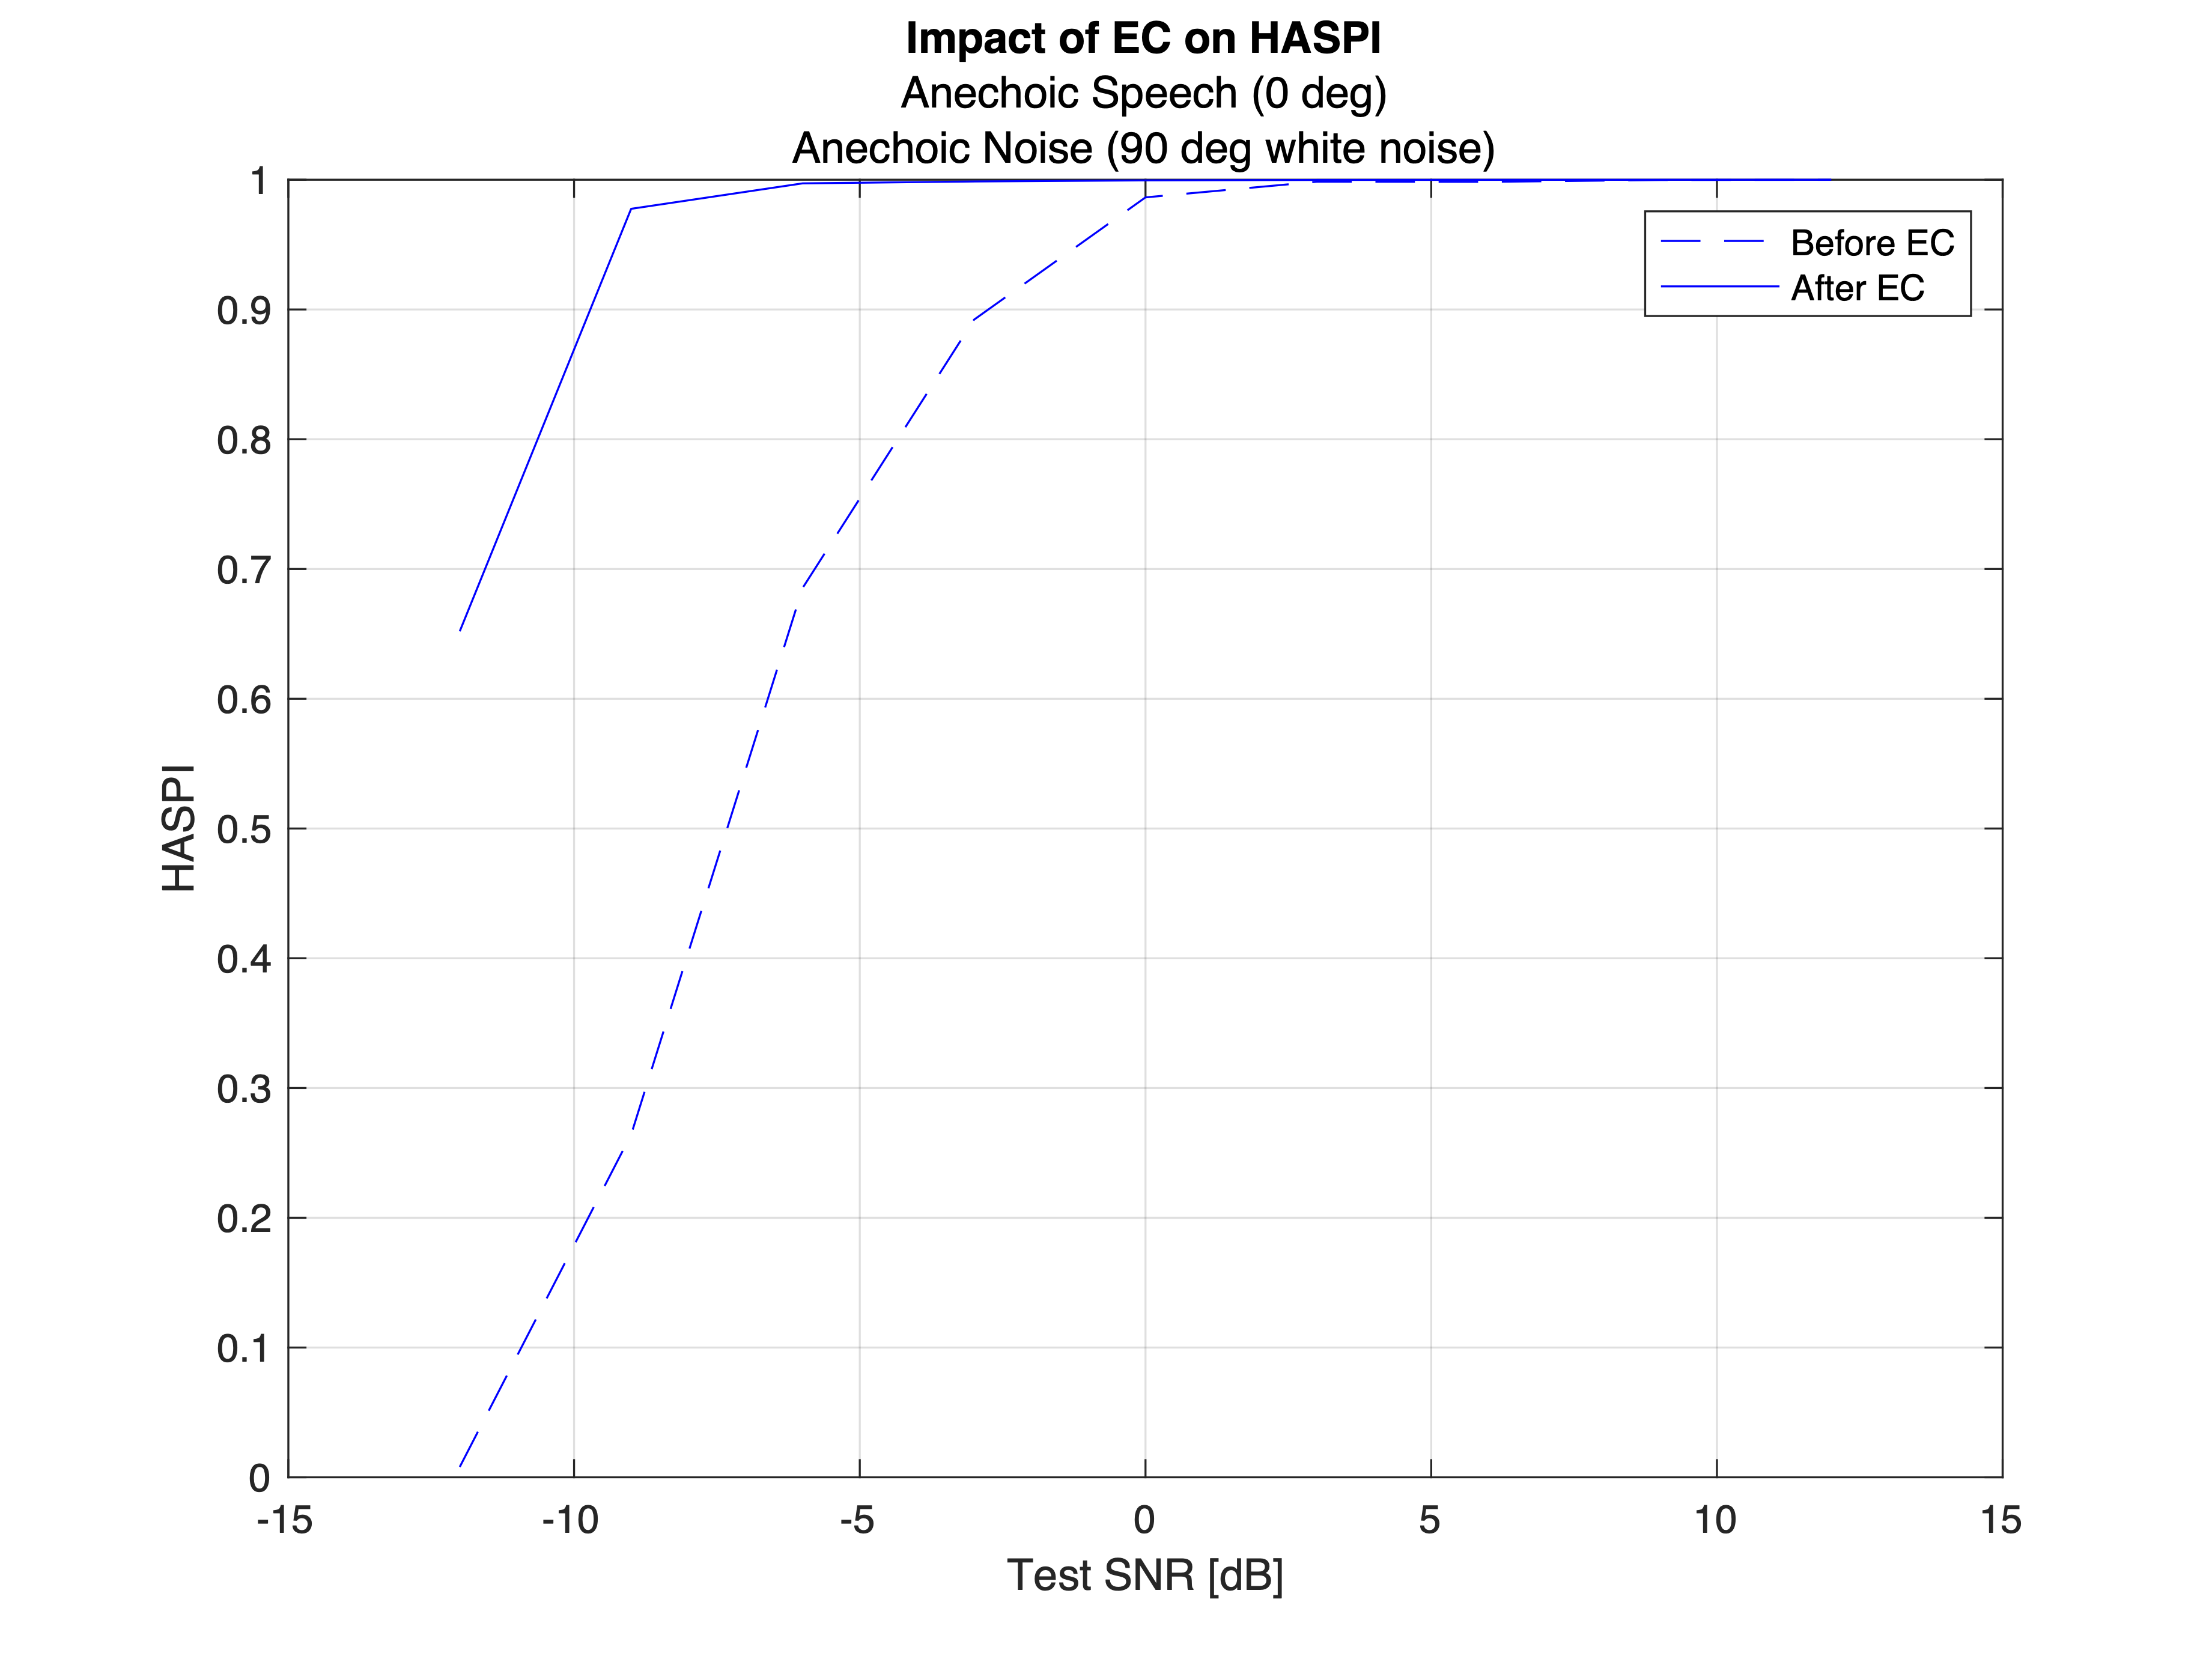
\includegraphics[width=\textwidth]{EC_SRM_AnechoicSpeech_AnechoicNoise}
	\end{subfigure}
	\hfill
	\begin{subfigure}[b]{0.49\textwidth}
		\centering
		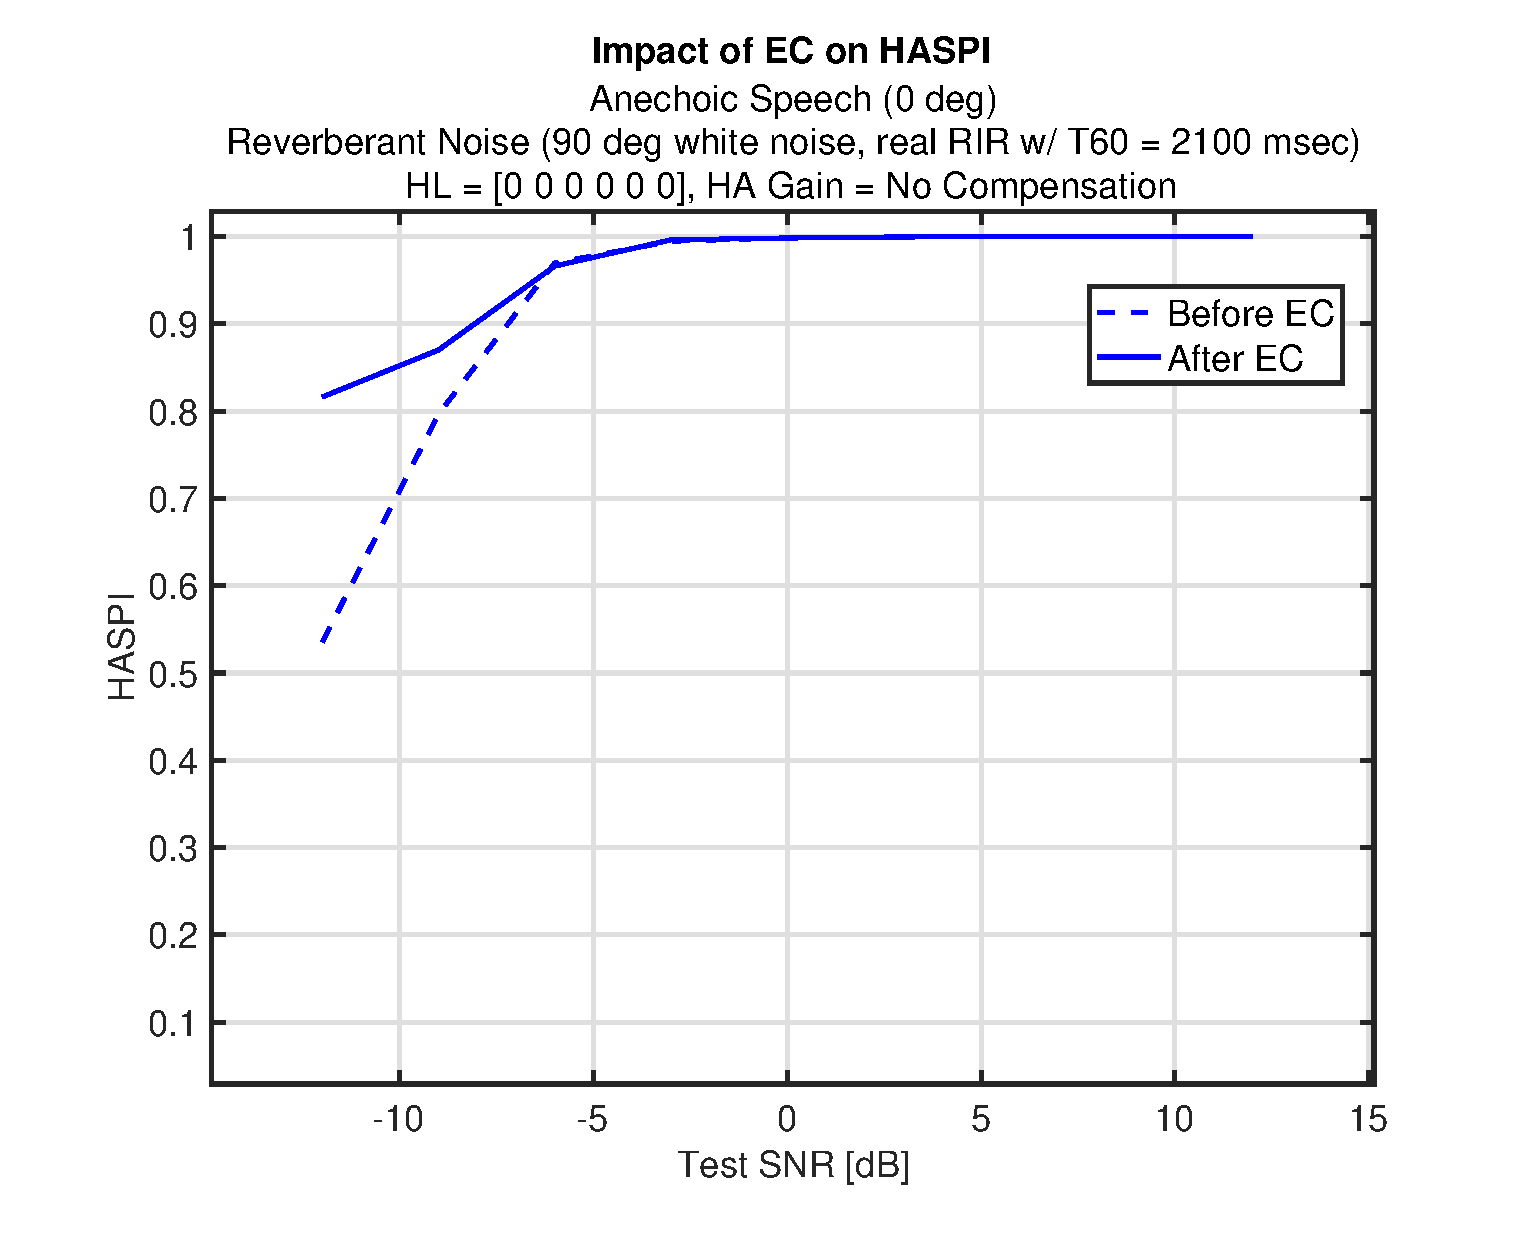
\includegraphics[width=\textwidth]{EC_SRM_AnechoicSpeech_ReverbNoise}
	\end{subfigure}
	\hfill
	\begin{subfigure}[b]{0.49\textwidth}
		\centering
		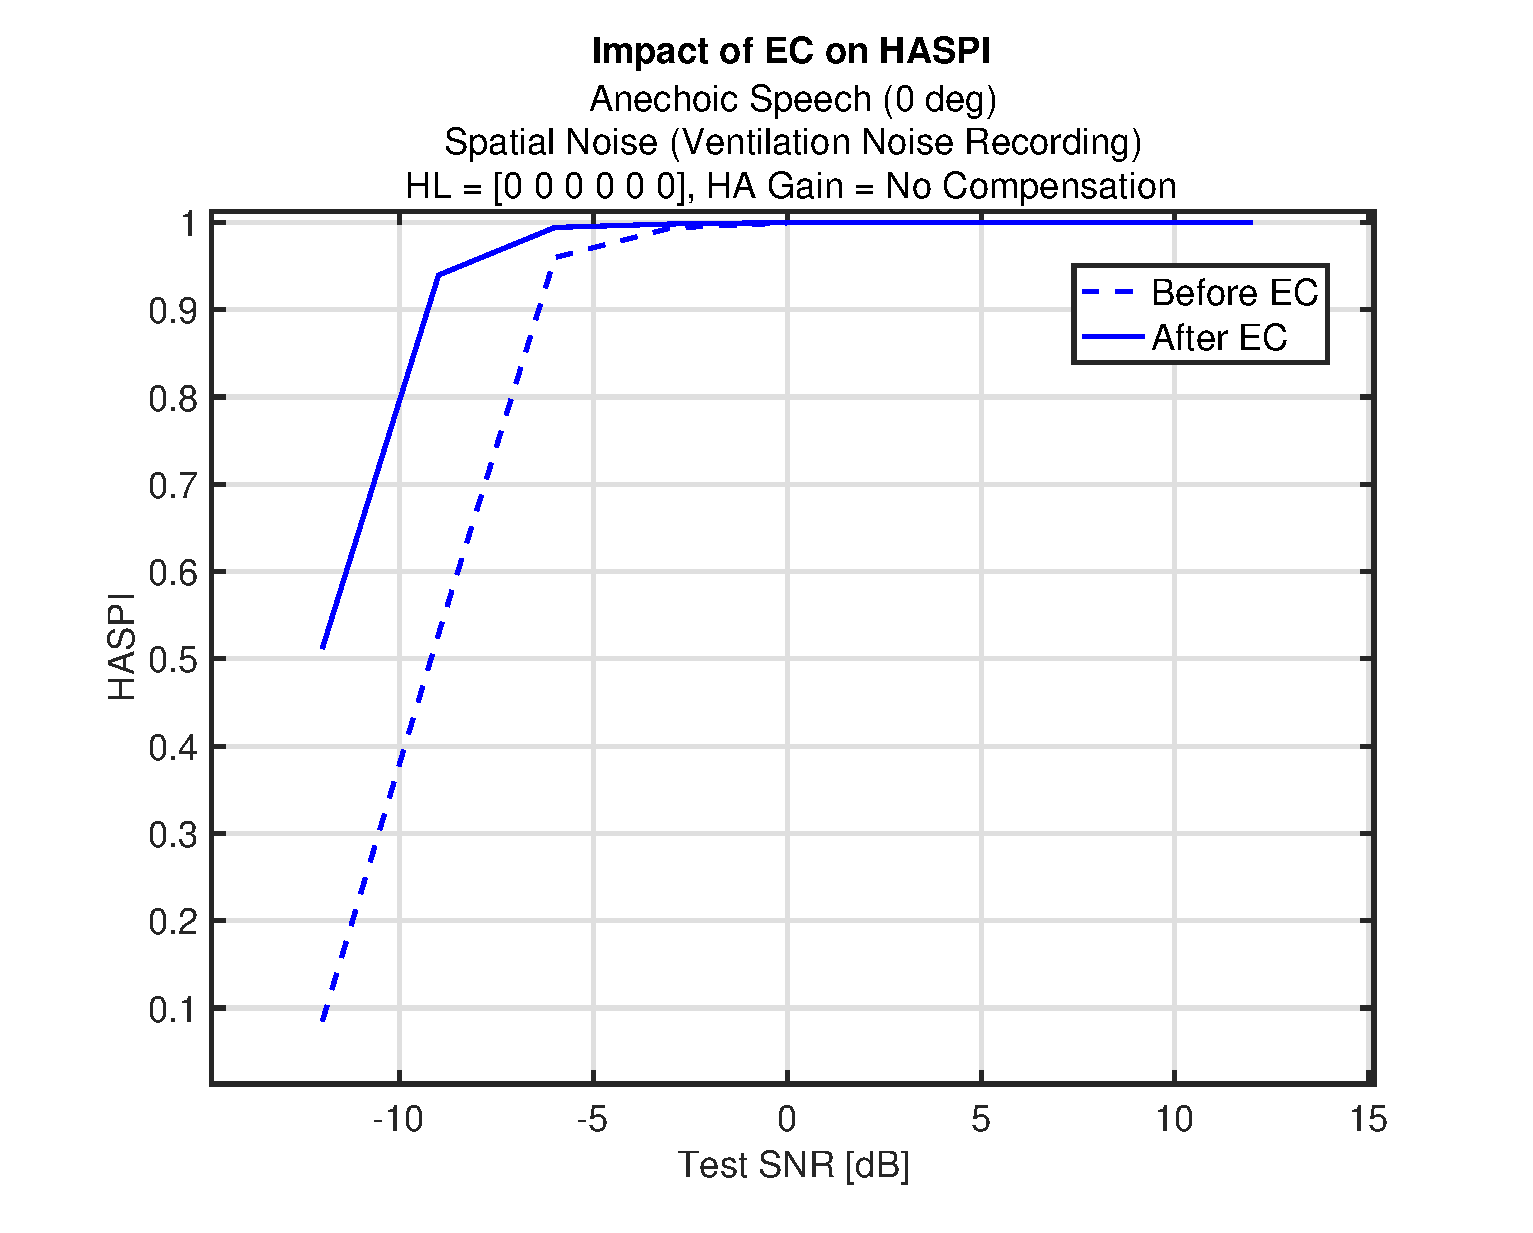
\includegraphics[width=\textwidth]{EC_SRM_AnechoicSpeech_SpatialNoiseRecording}
	\end{subfigure}
	\hfill
	\begin{subfigure}[b]{0.49\textwidth}
		\centering
		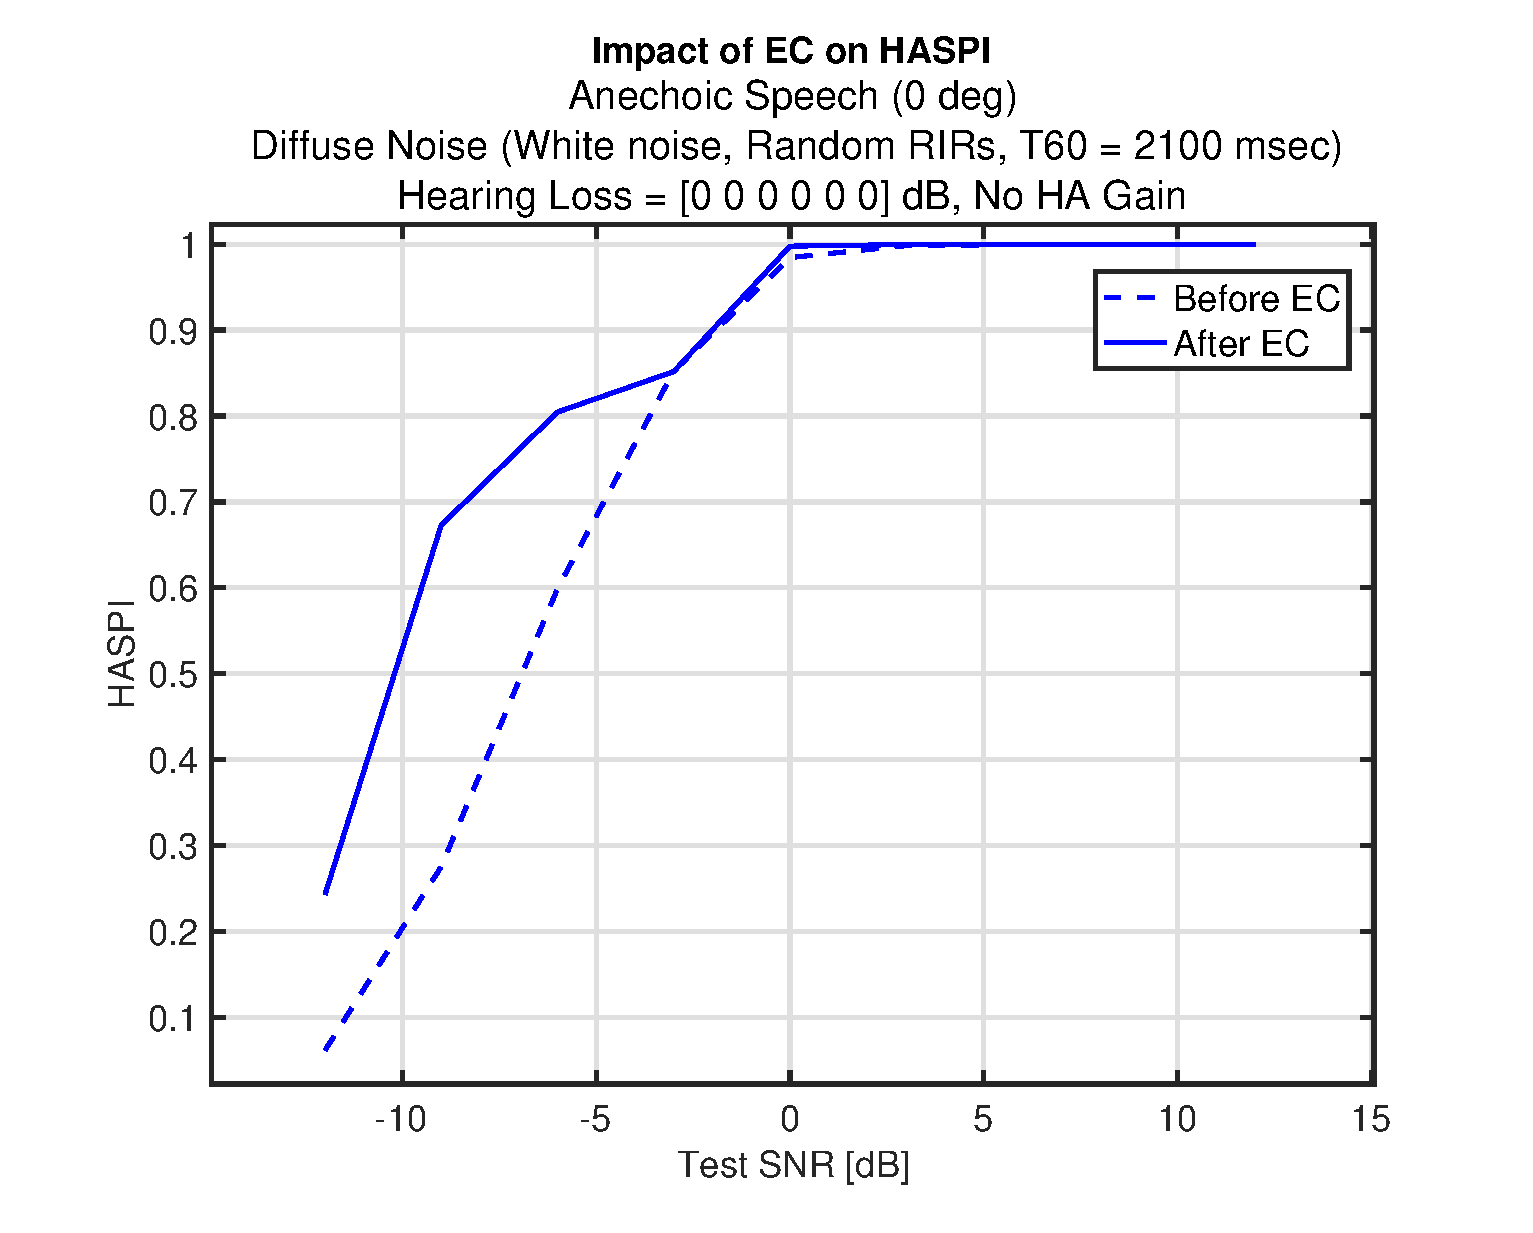
\includegraphics[width=\textwidth]{EC_SRM_AnechoicSpeech_DiffuseNoise}
	\end{subfigure}
	\hfill
	\caption{Impact of EC algorithm on speech intelligibility (using HASPI) as a function of SNR, for anechoic directional speech and various noise types (anechoic directional, reverberant, spatial recording, diffuse)}
	\label{fig:EC_SRM_AnechoicSpeech}
\end{figure}


\begin{figure}[H]
	\centering
	\begin{subfigure}[b]{0.49\textwidth}
		\centering
		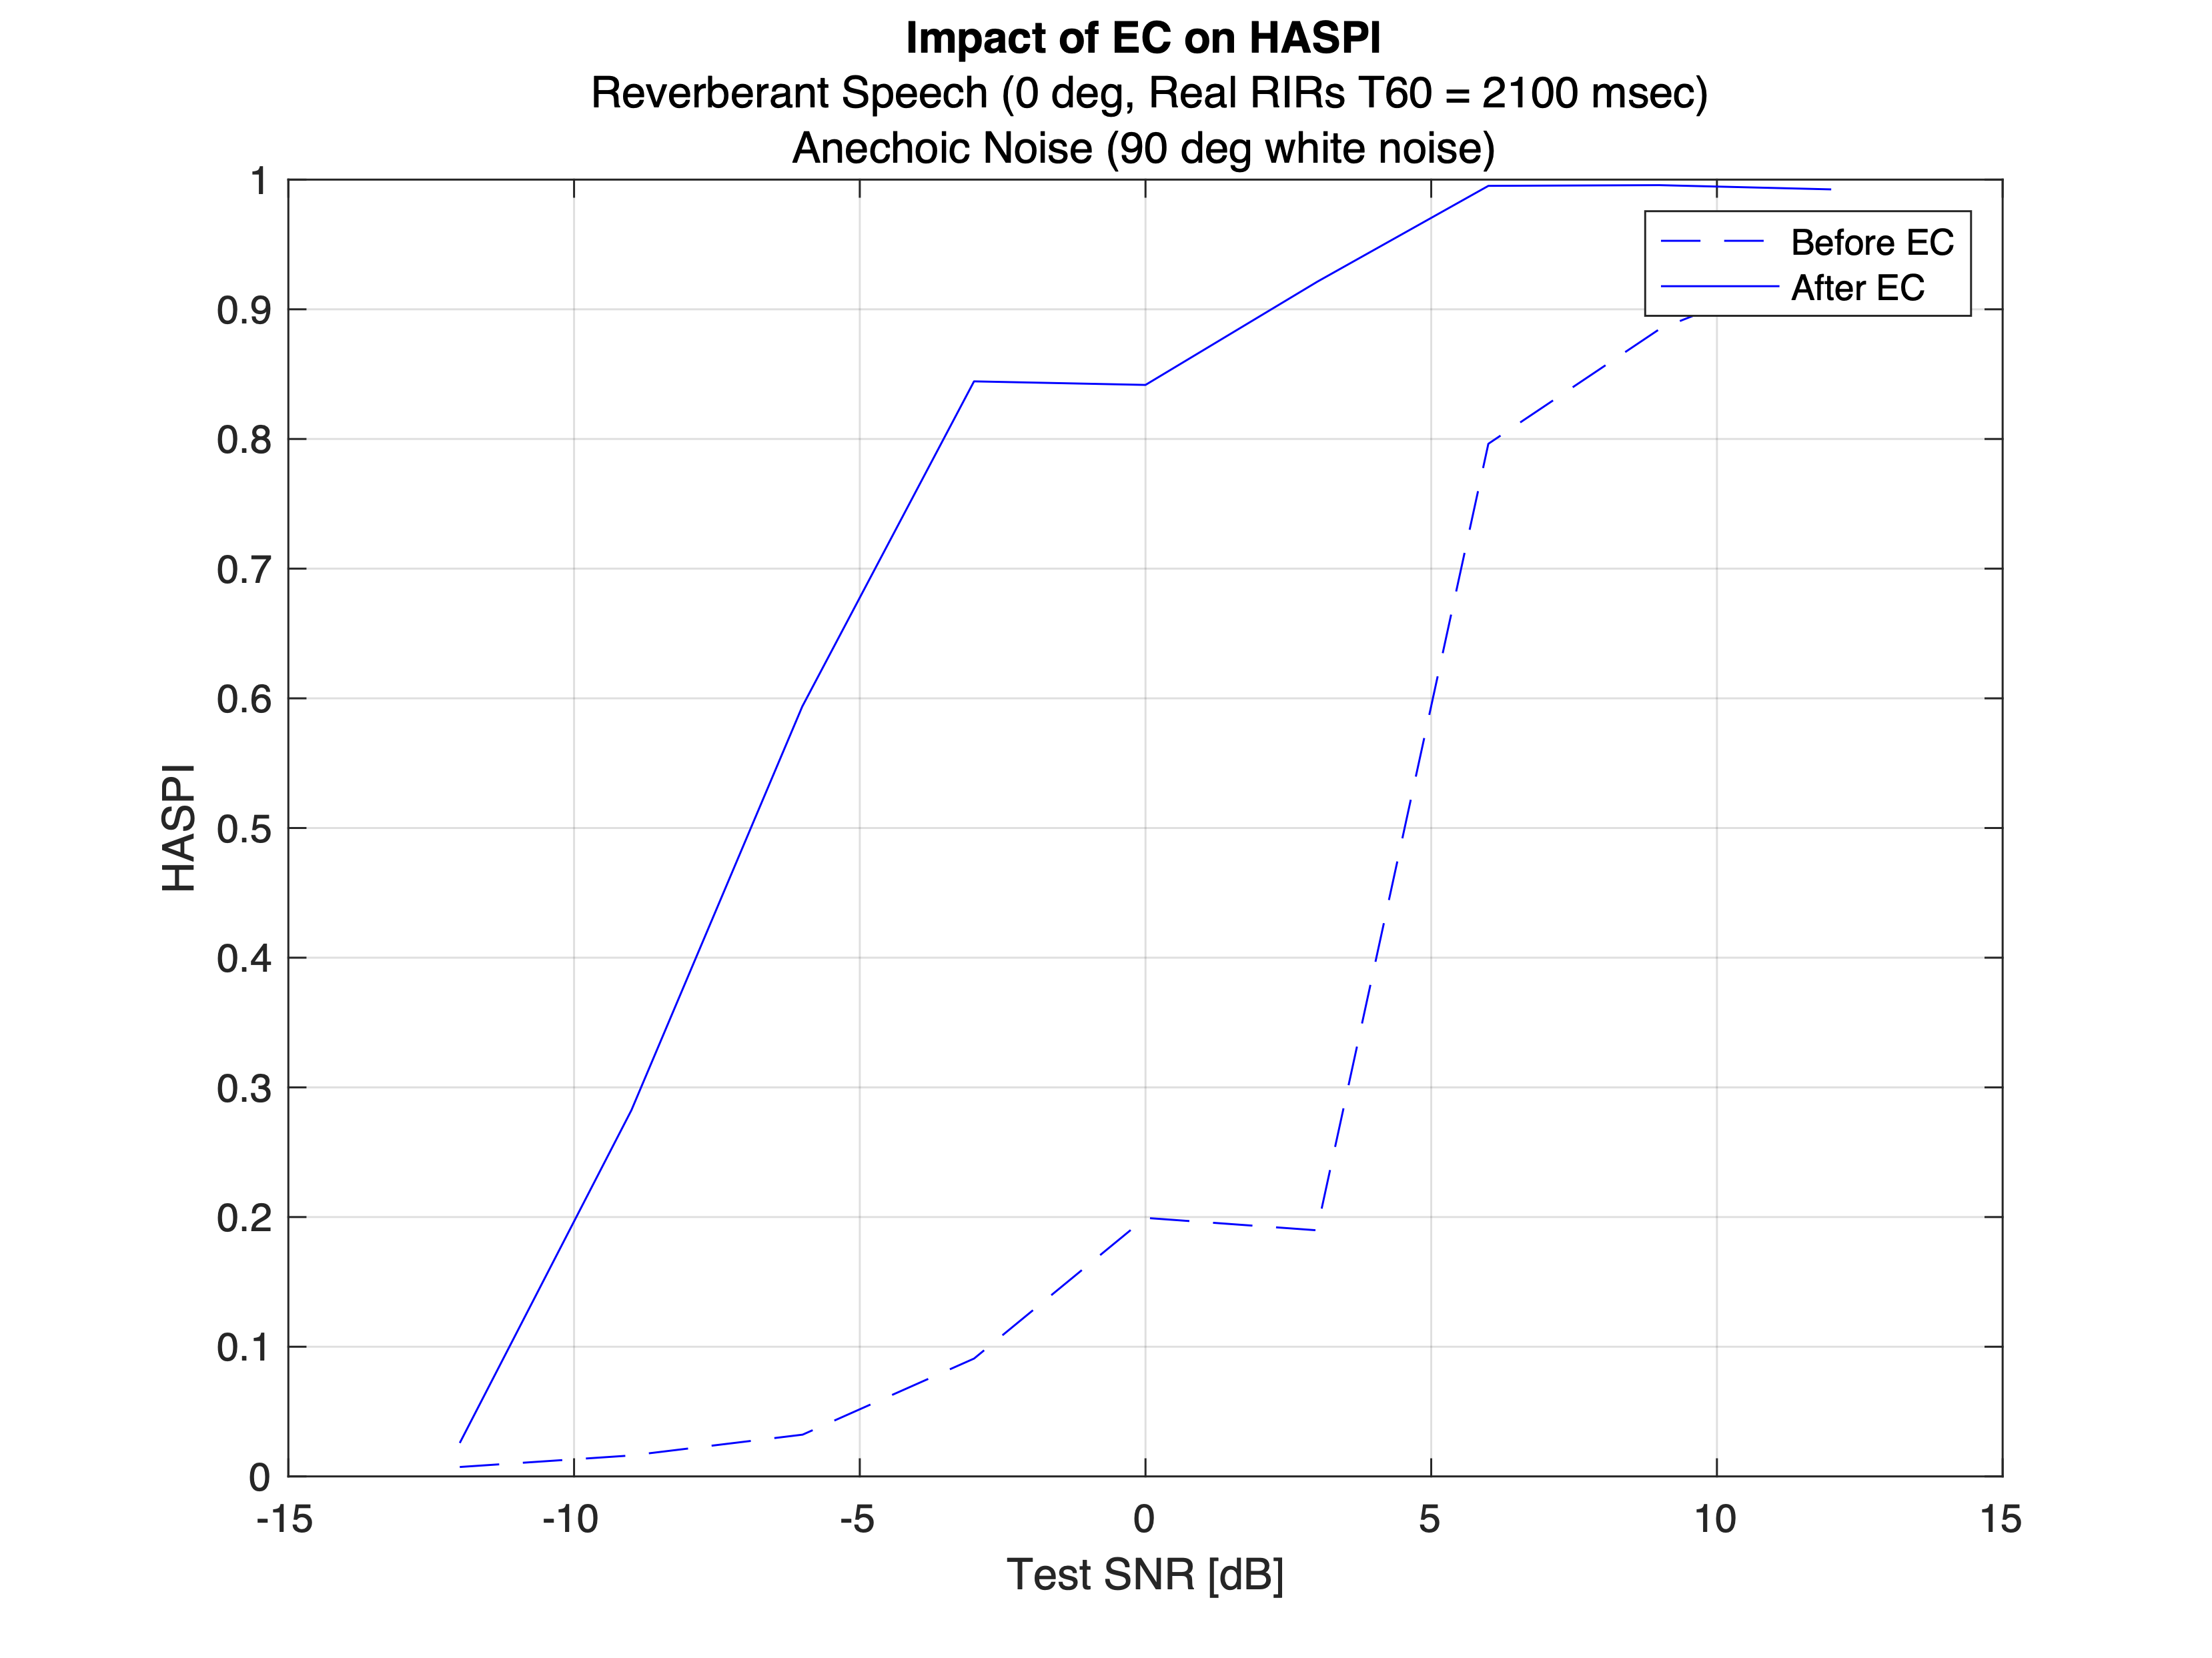
\includegraphics[width=\textwidth]{EC_SRM_ReverbSpeech_AnechoicNoise}
	\end{subfigure}
	\hfill
	\begin{subfigure}[b]{0.49\textwidth}
		\centering
		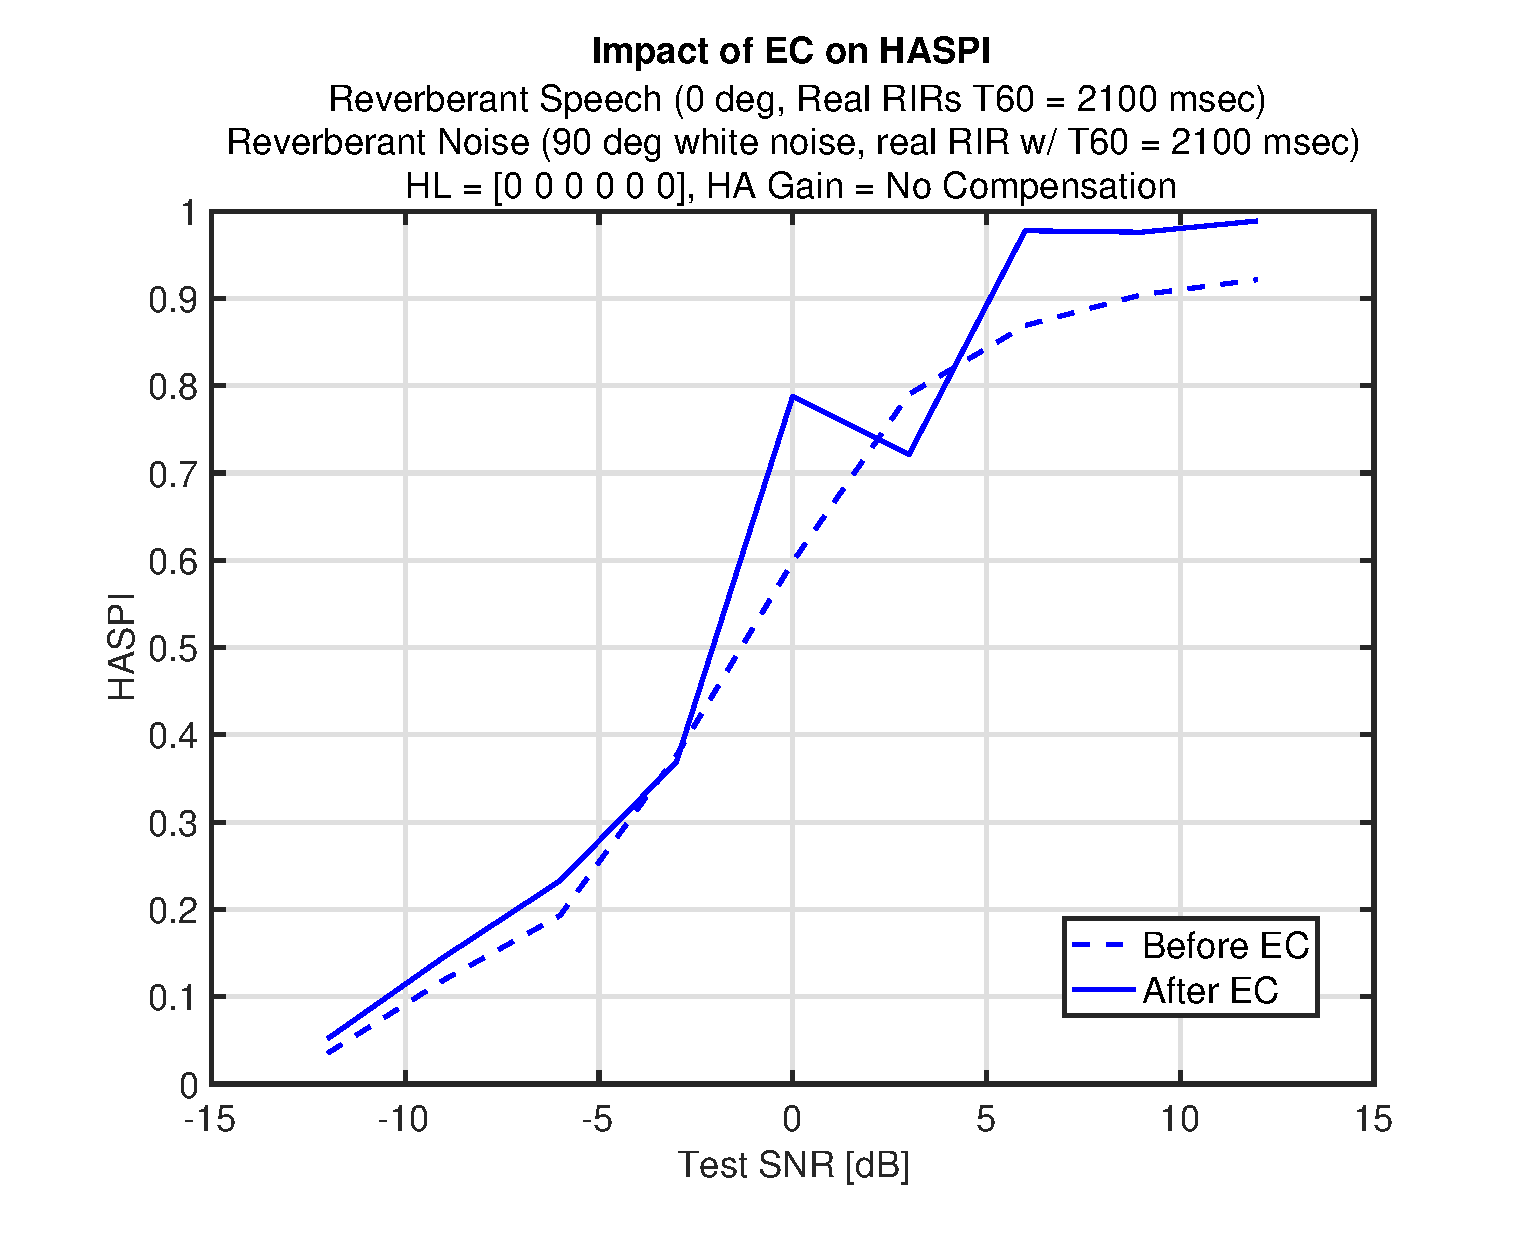
\includegraphics[width=\textwidth]{EC_SRM_ReverbSpeech_ReverbNoise}
	\end{subfigure}
	\hfill
	\begin{subfigure}[b]{0.49\textwidth}
		\centering
		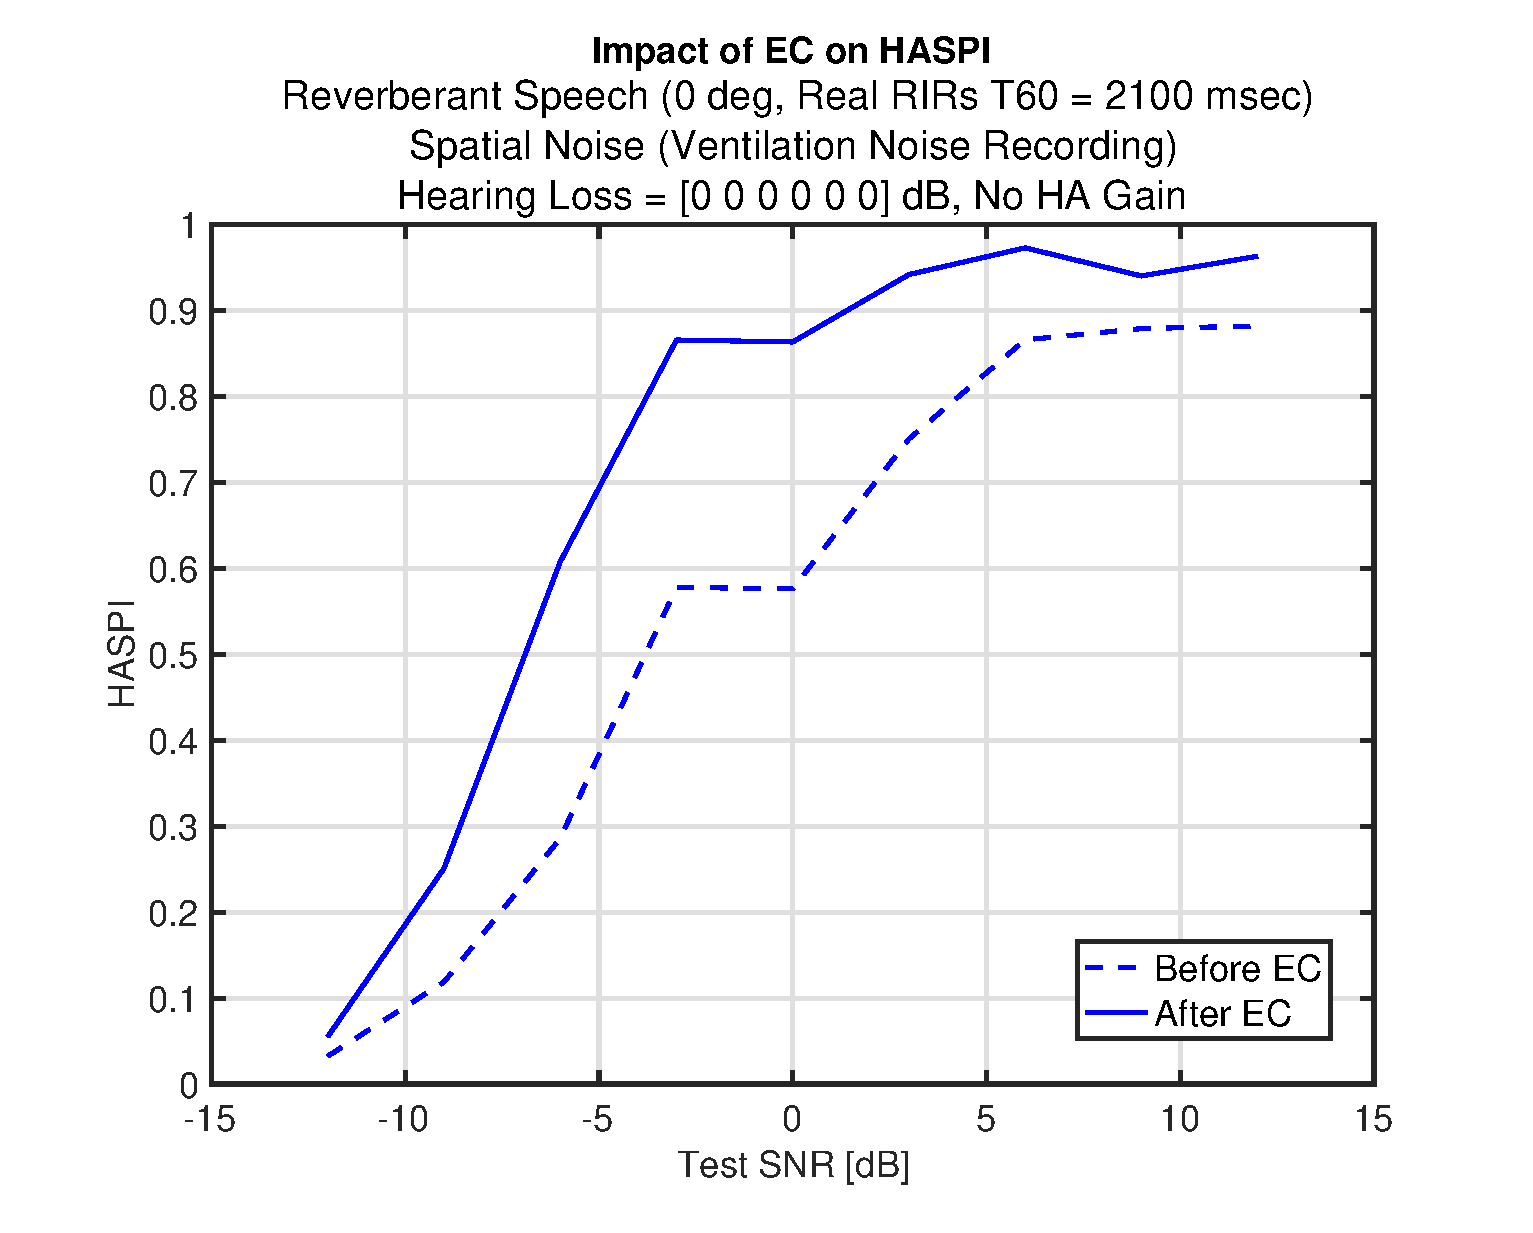
\includegraphics[width=\textwidth]{EC_SRM_ReverbSpeech_SpatialNoiseRecording}
	\end{subfigure}
	\hfill
	\begin{subfigure}[b]{0.49\textwidth}
		\centering
		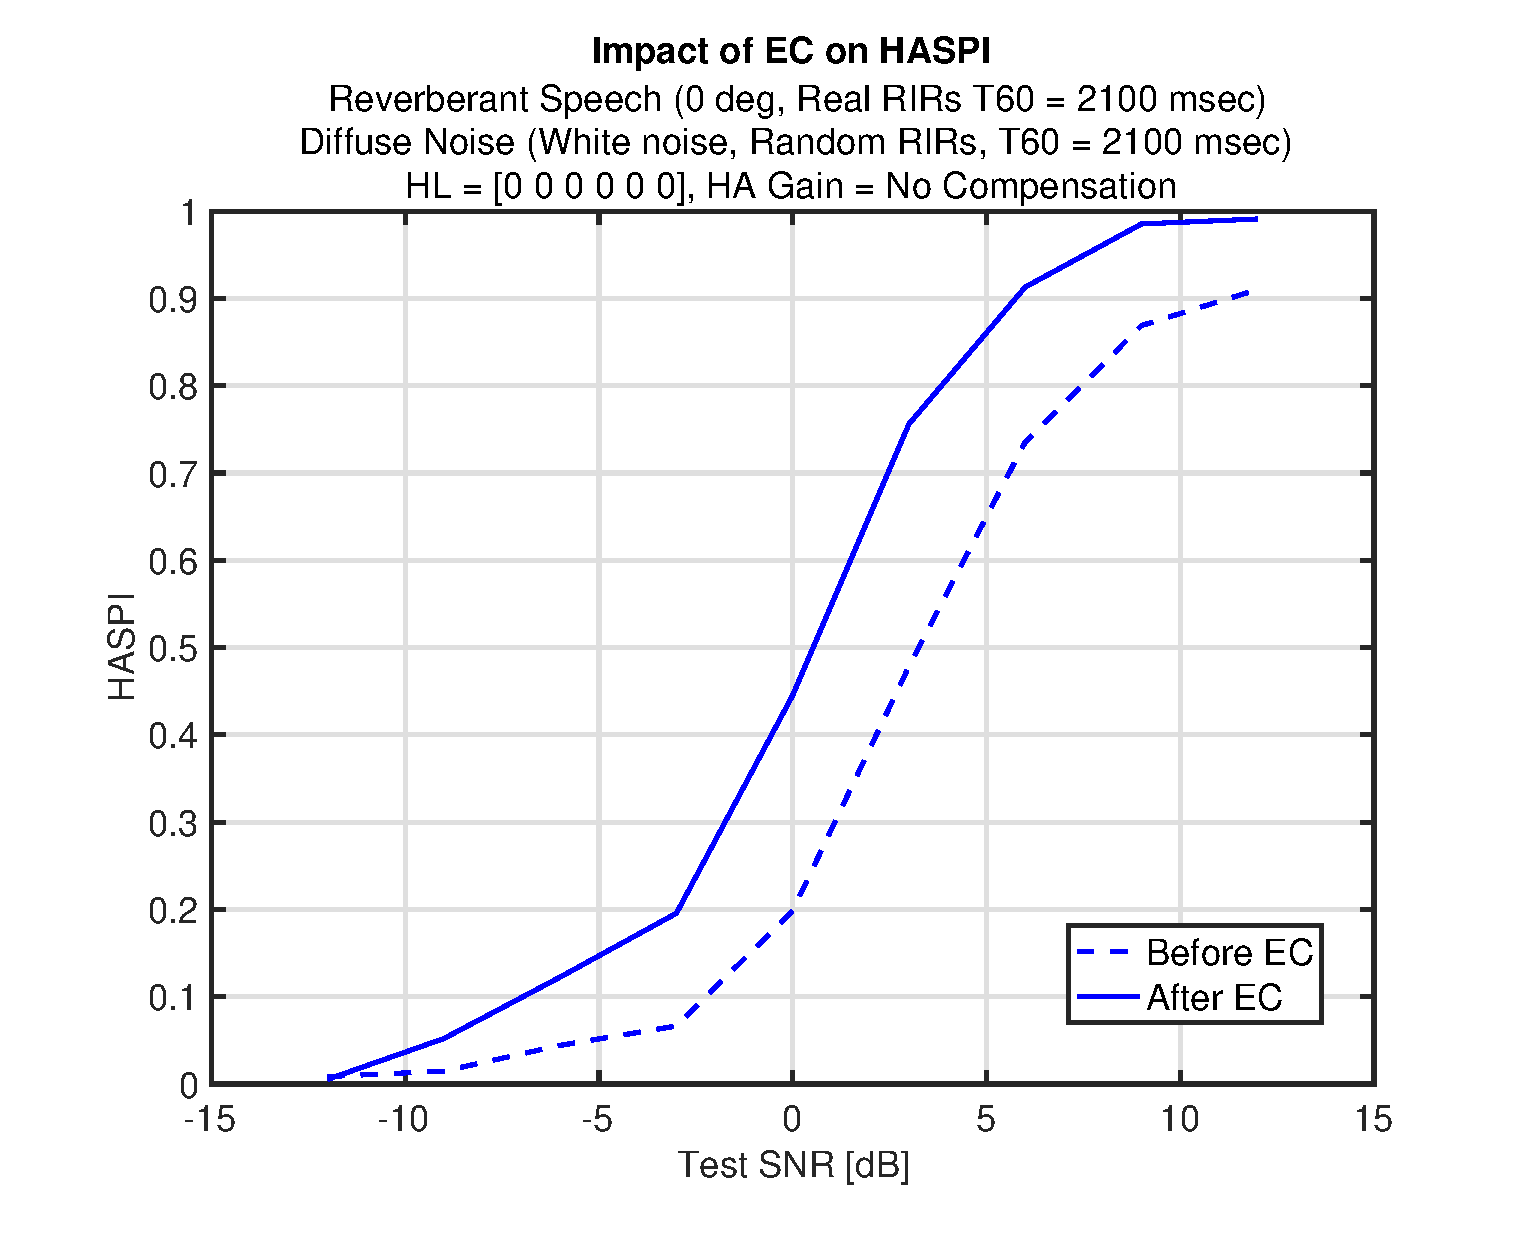
\includegraphics[width=\textwidth]{EC_SRM_ReverbSpeech_DiffuseNoise}
	\end{subfigure}
	\hfill
	\caption{Impact of EC algorithm on speech intelligibility (using HASPI) as a function of SNR, for reverberant speech and various noise types (anechoic directional, reverberant, spatial recording, diffuse)}
	\label{fig:EC_SRM_ReverbSpeech}
\end{figure}


\begin{figure}[H]
	\centering
	\begin{subfigure}[b]{0.49\textwidth}
		\centering
		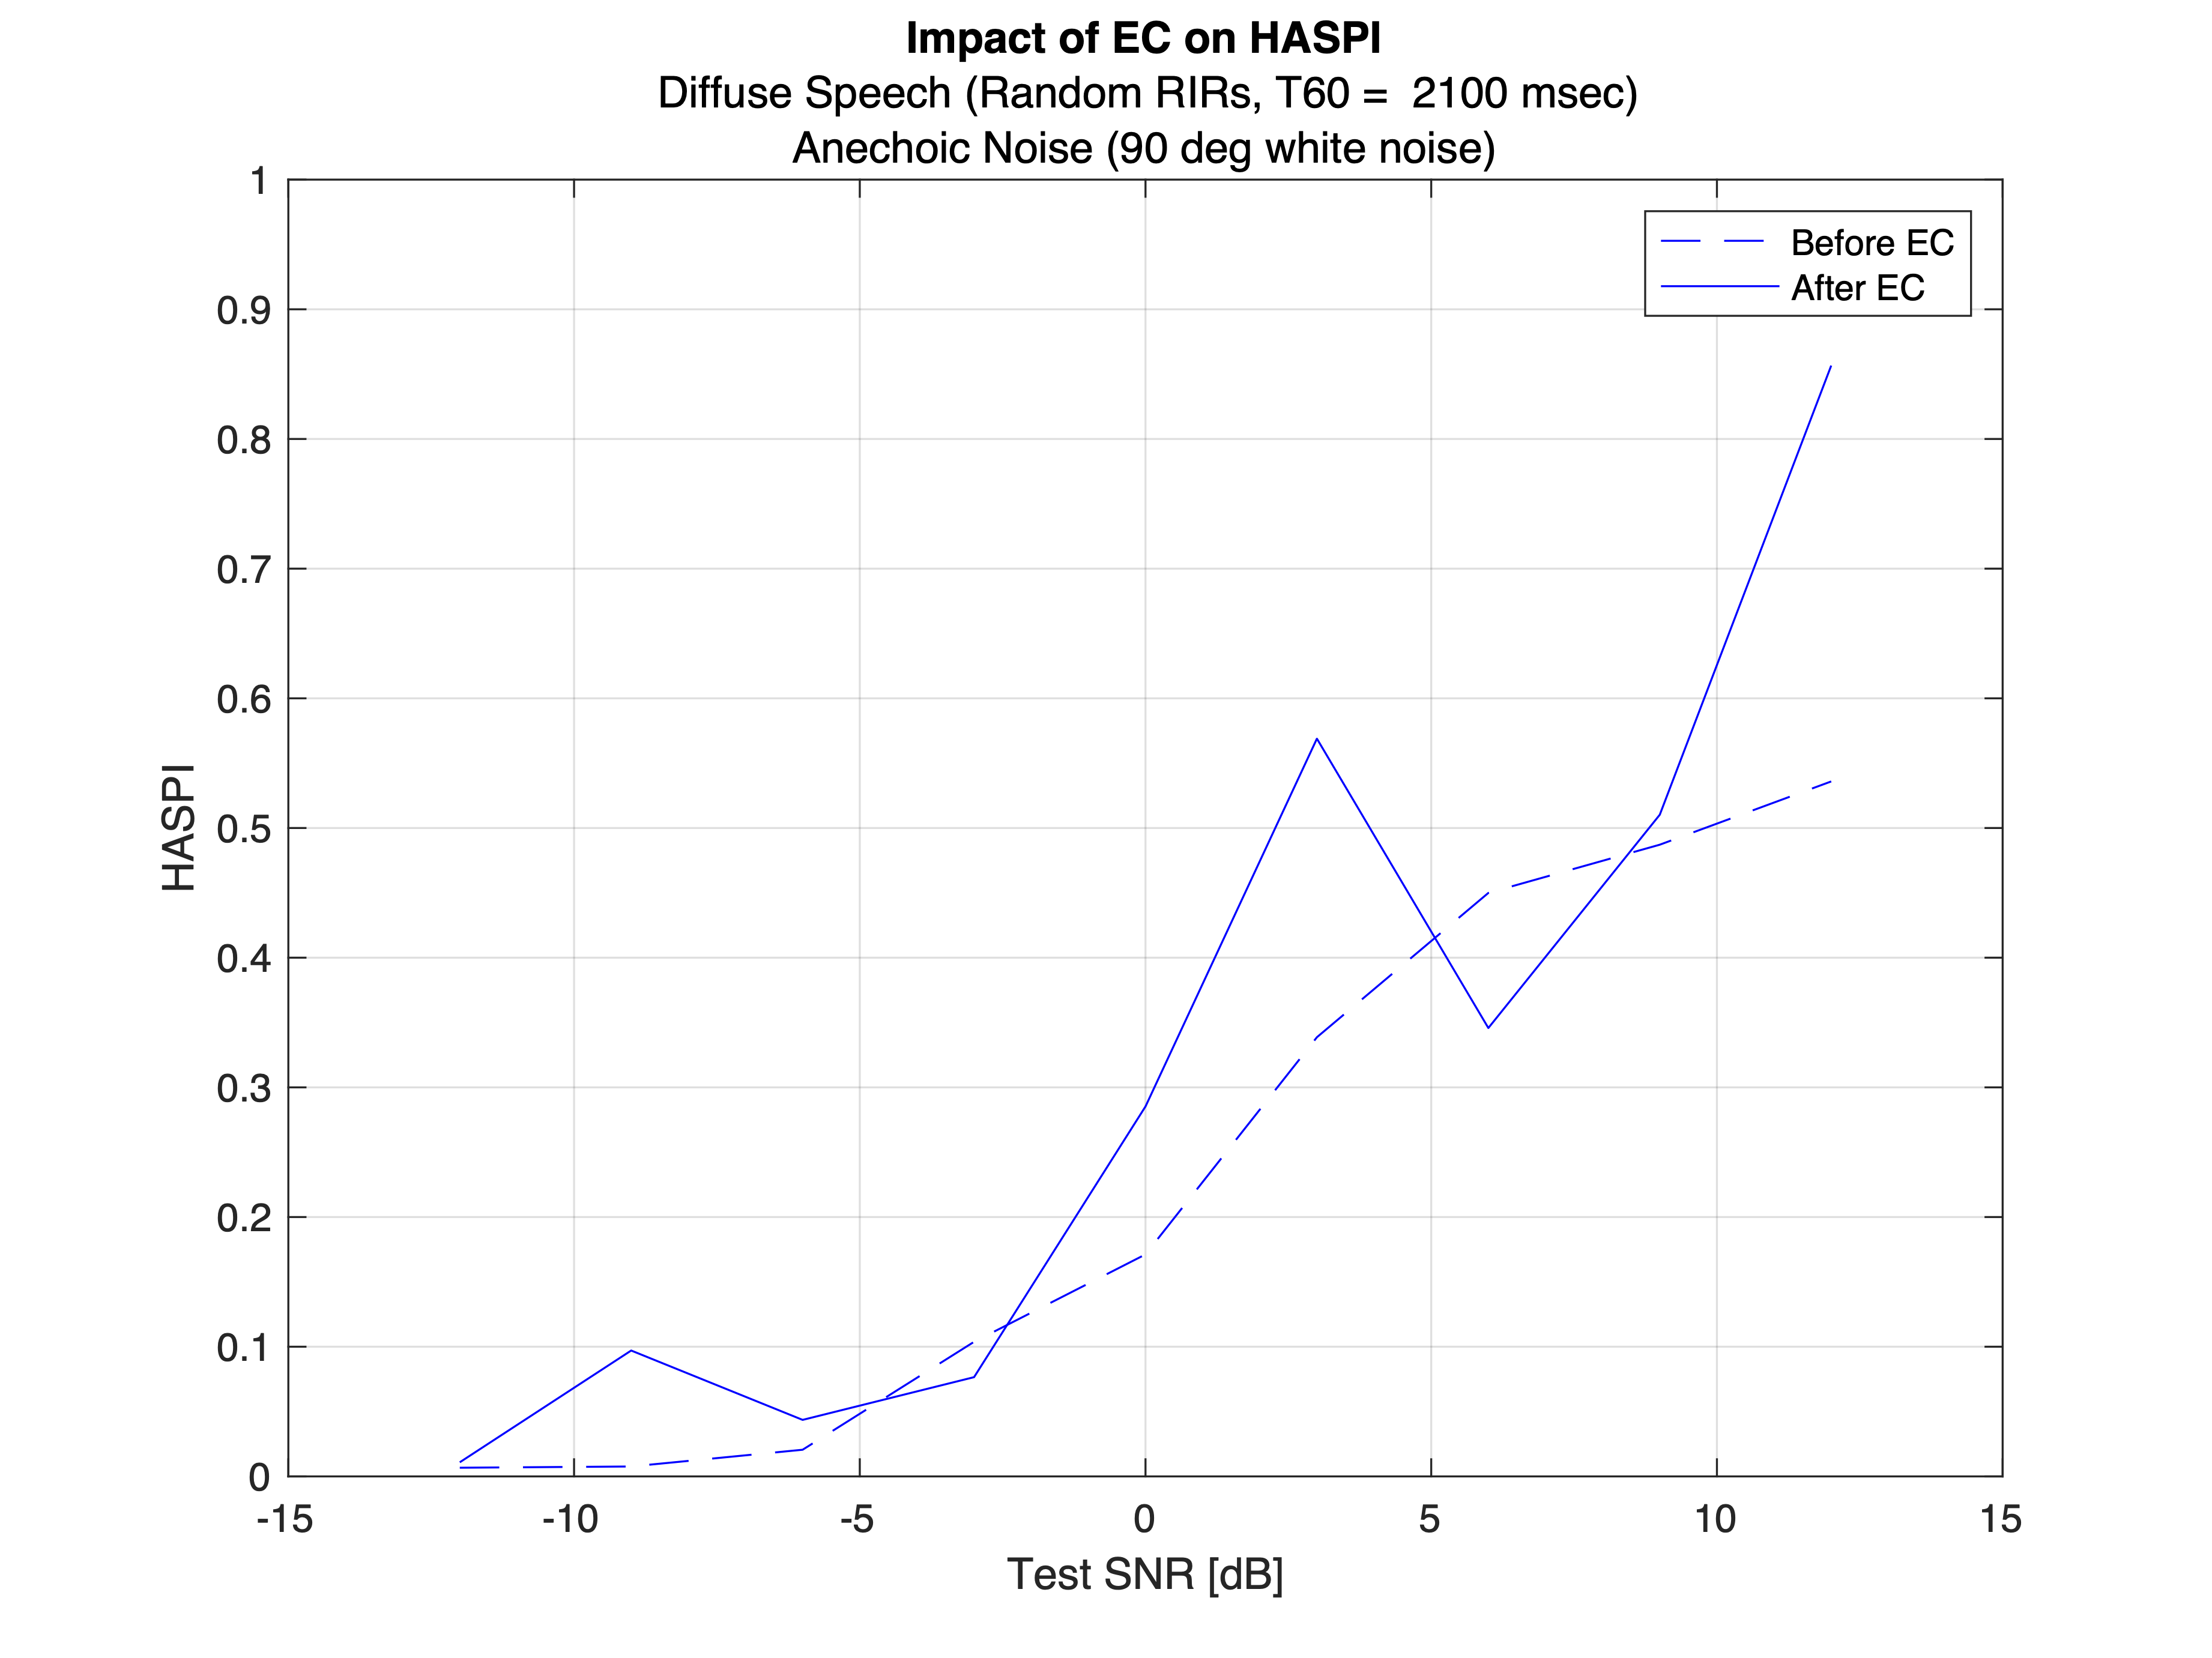
\includegraphics[width=\textwidth]{EC_SRM_DiffuseSpeech_AnechoicNoise}
	\end{subfigure}
	\hfill
	\begin{subfigure}[b]{0.49\textwidth}
		\centering
		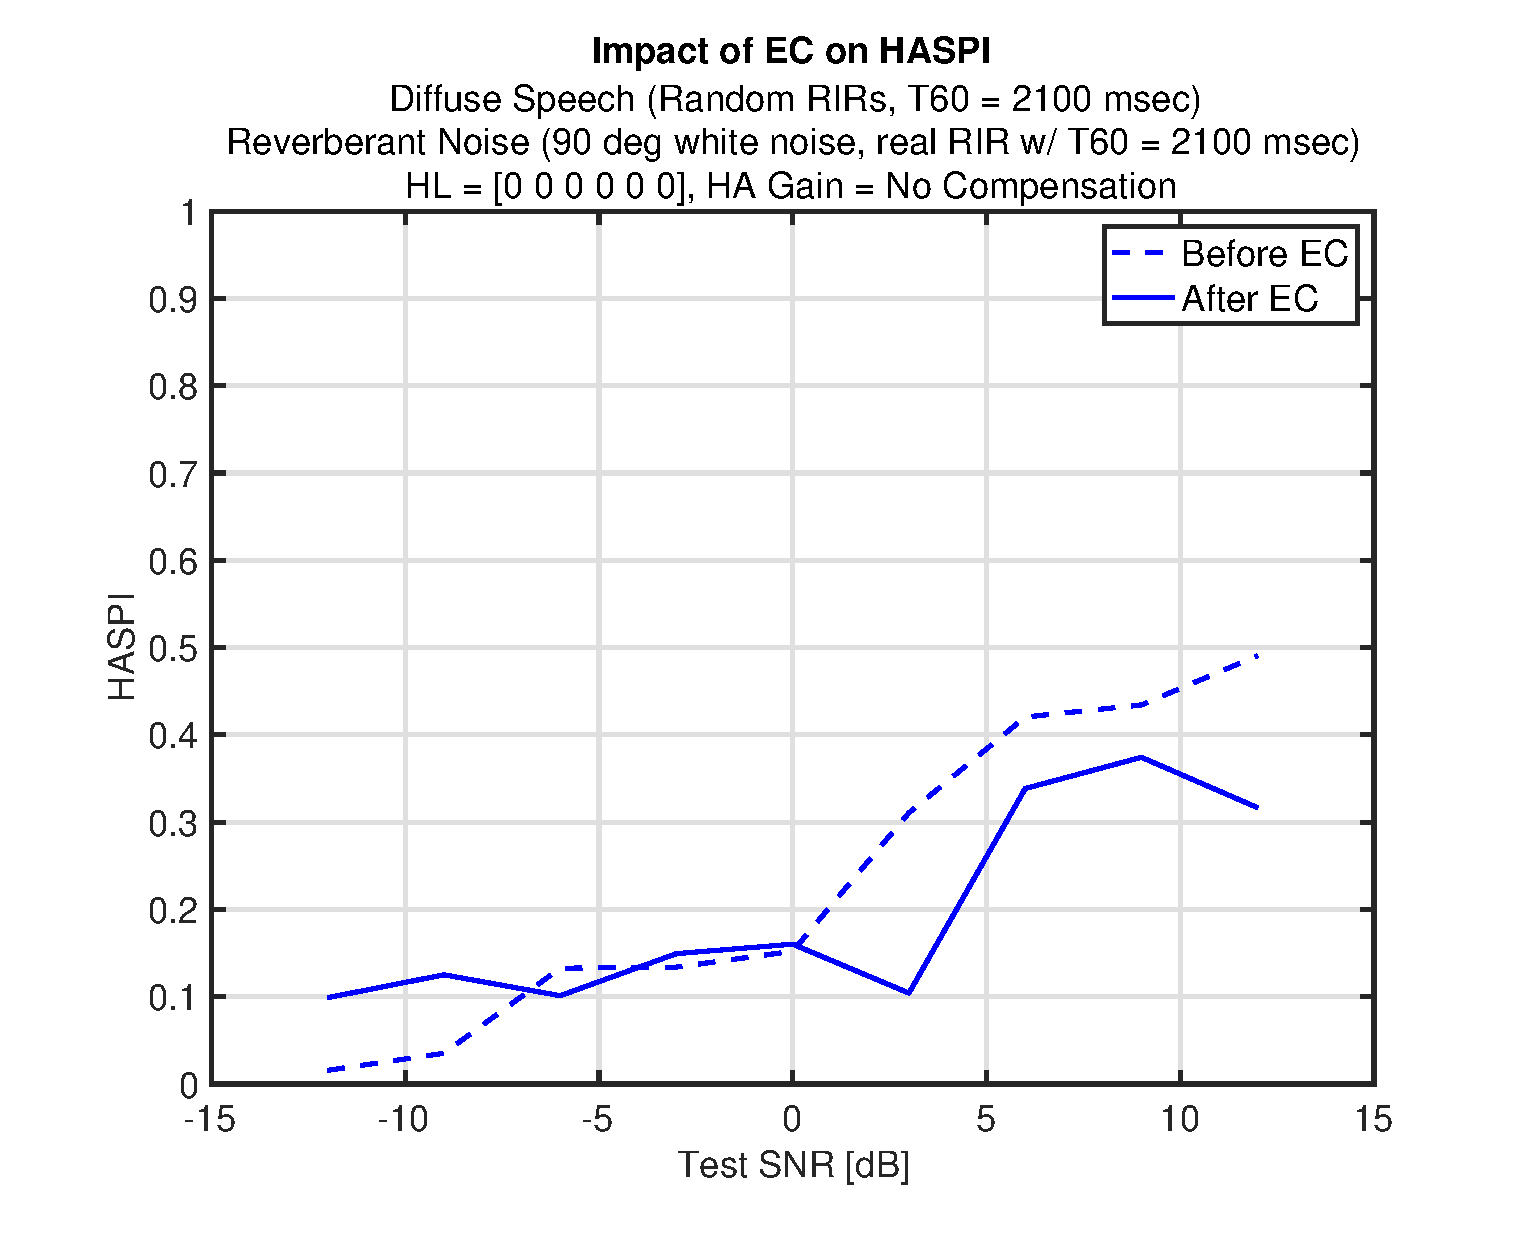
\includegraphics[width=\textwidth]{EC_SRM_DiffuseSpeech_ReverbNoise}
	\end{subfigure}
	\hfill
	\begin{subfigure}[b]{0.49\textwidth}
		\centering
		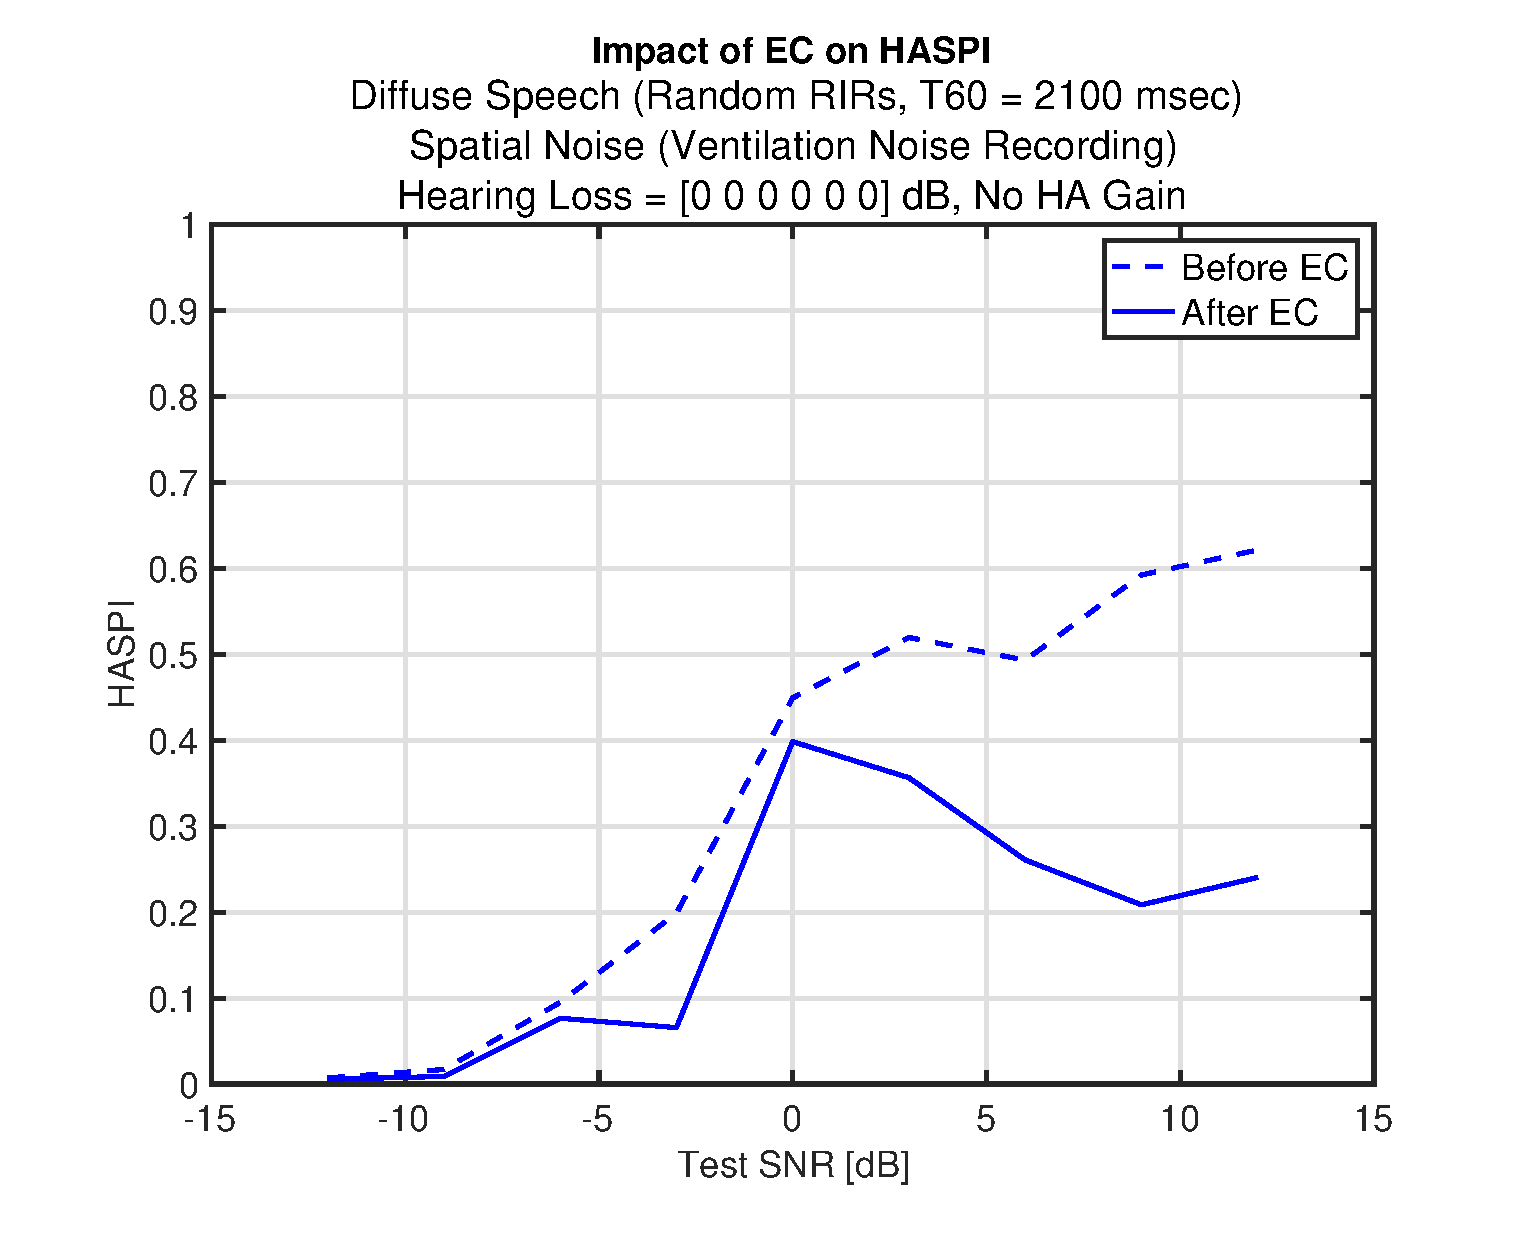
\includegraphics[width=\textwidth]{EC_SRM_DiffuseSpeech_SpatialNoiseRecording}
	\end{subfigure}
	\hfill
	\begin{subfigure}[b]{0.49\textwidth}
		\centering
		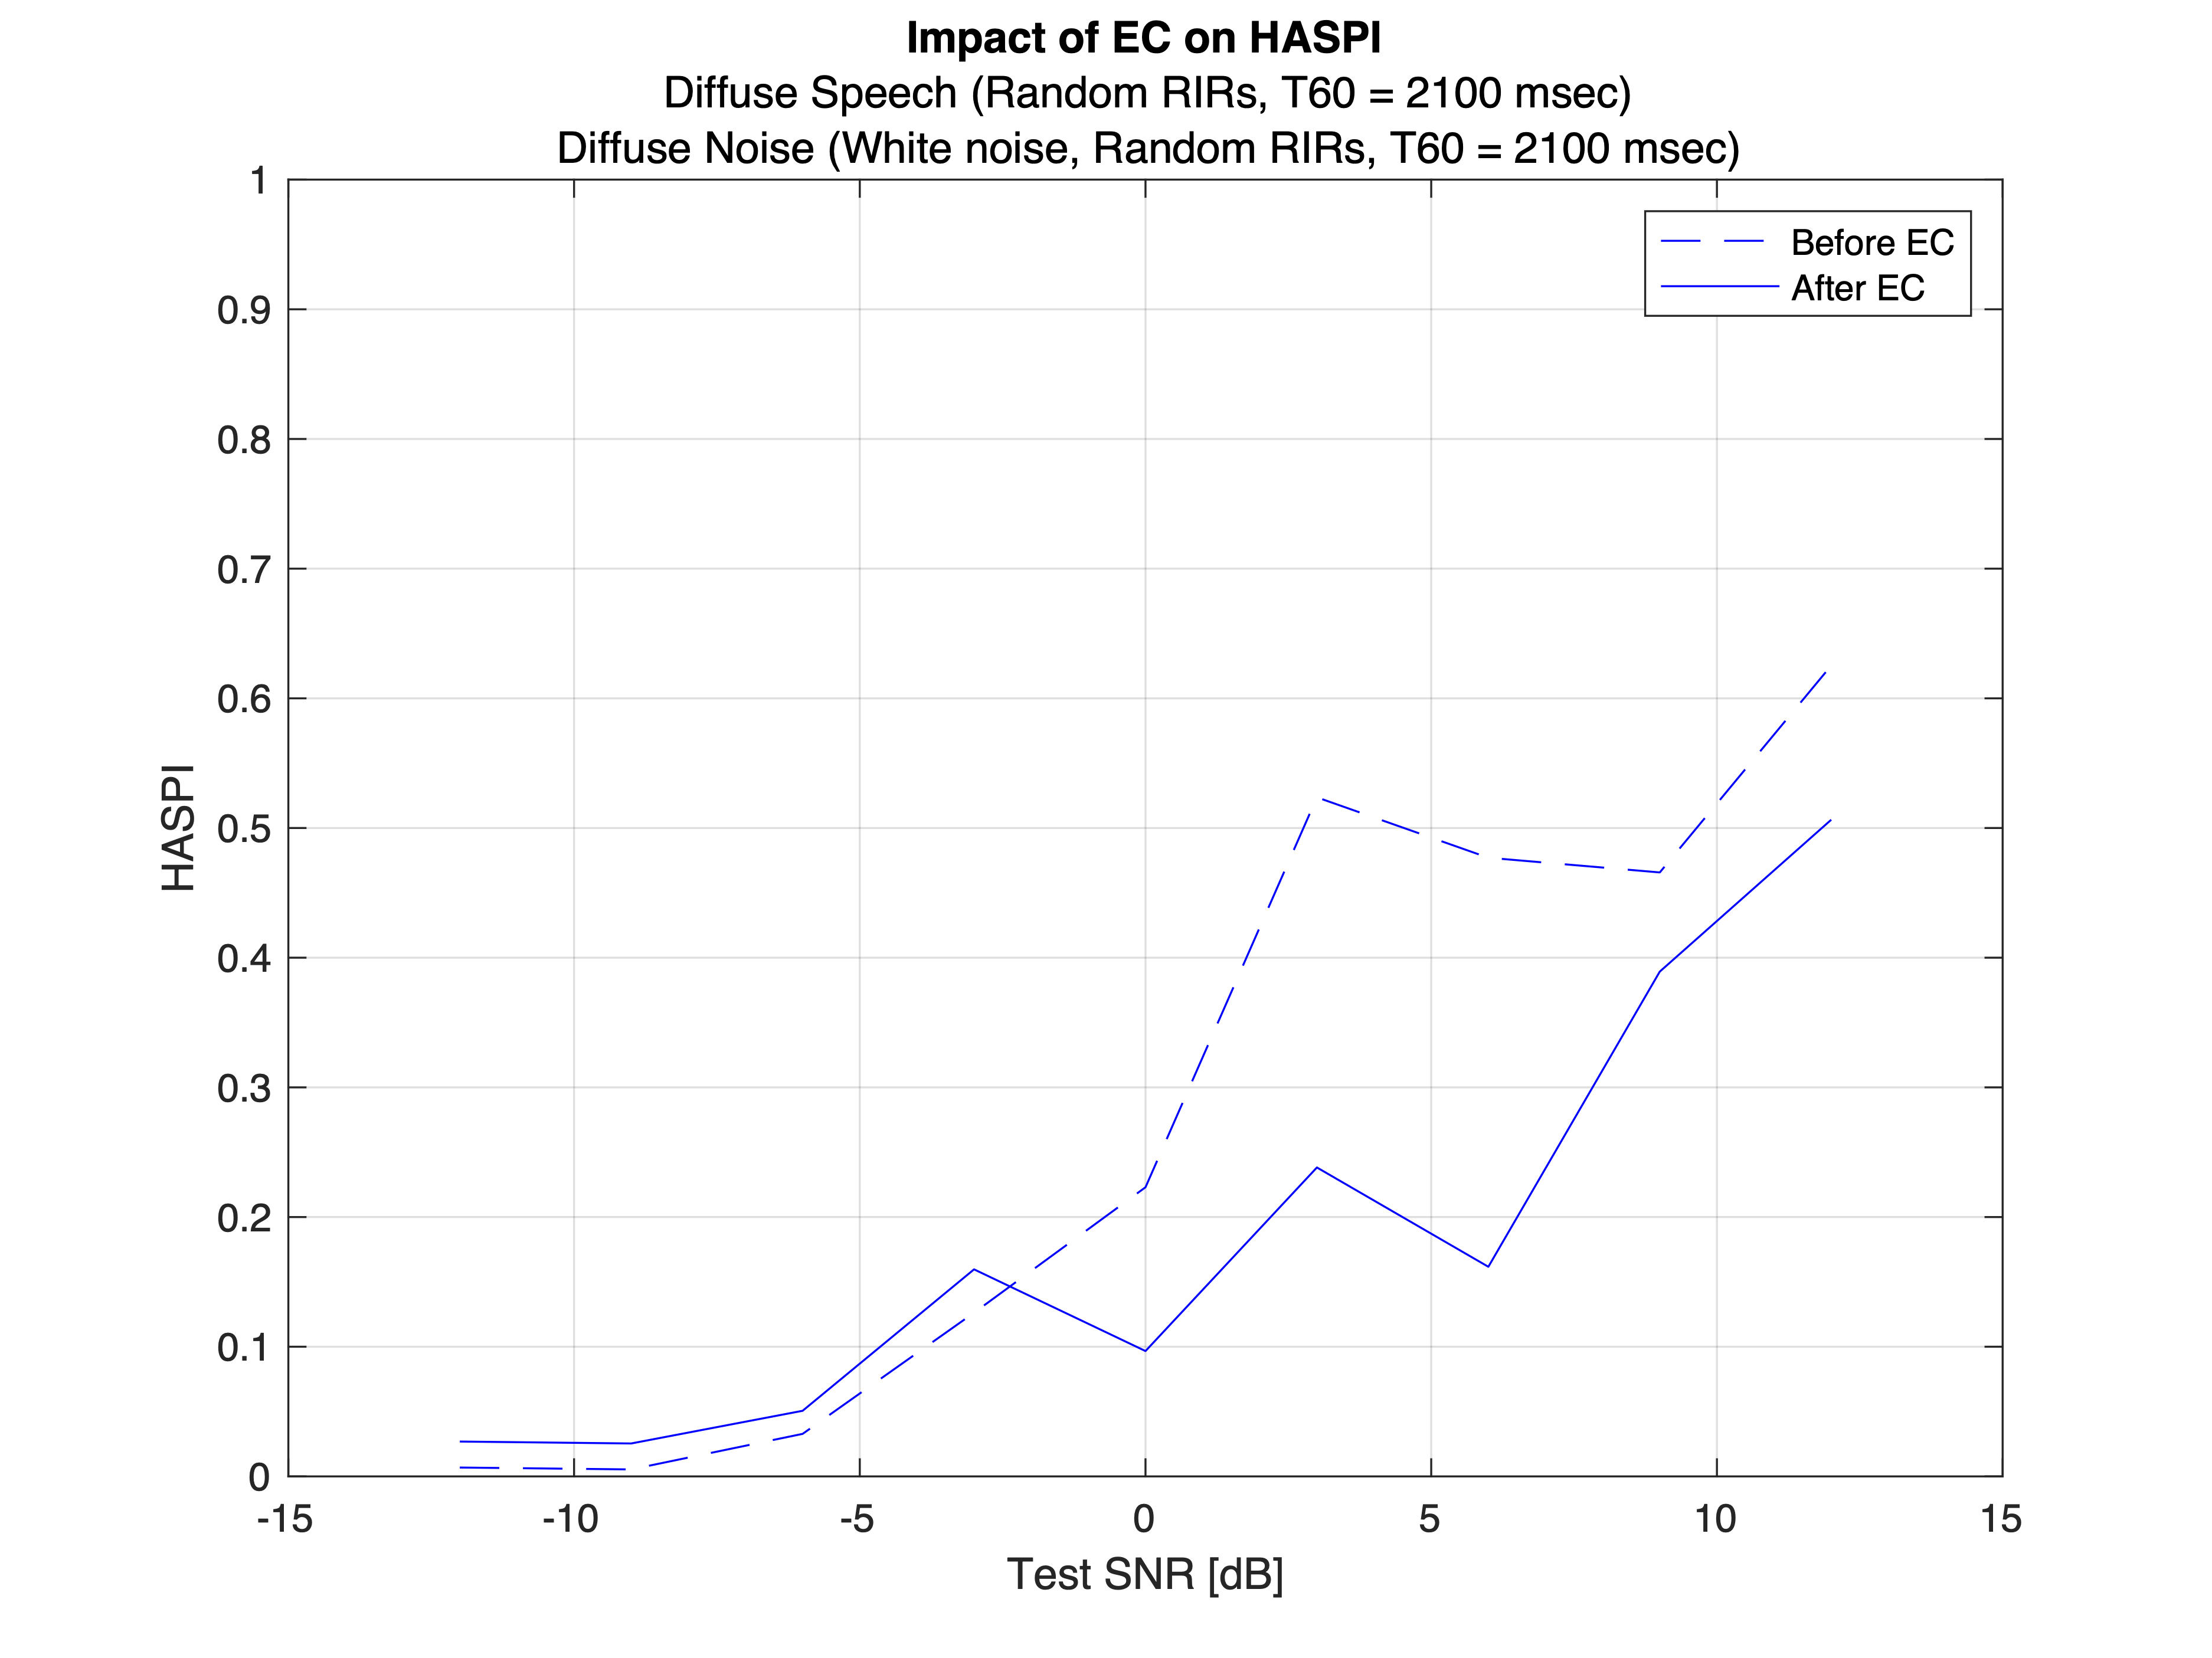
\includegraphics[width=\textwidth]{EC_SRM_DiffuseSpeech_DiffuseNoise}
	\end{subfigure}
	\hfill
	\caption{Impact of EC algorithm on speech intelligibility (using HASPI) as a function of SNR, for diffuse speech and various noise types (anechoic directional, reverberant, spatial recording, diffuse)}
	\label{fig:EC_SRM_DiffuseSpeech}
\end{figure}


\textbf{Impact of reverb on binaural benefit modeled by EC}


\begin{figure}[H]
	\centering
	\begin{subfigure}[b]{0.49\textwidth}
		\centering
		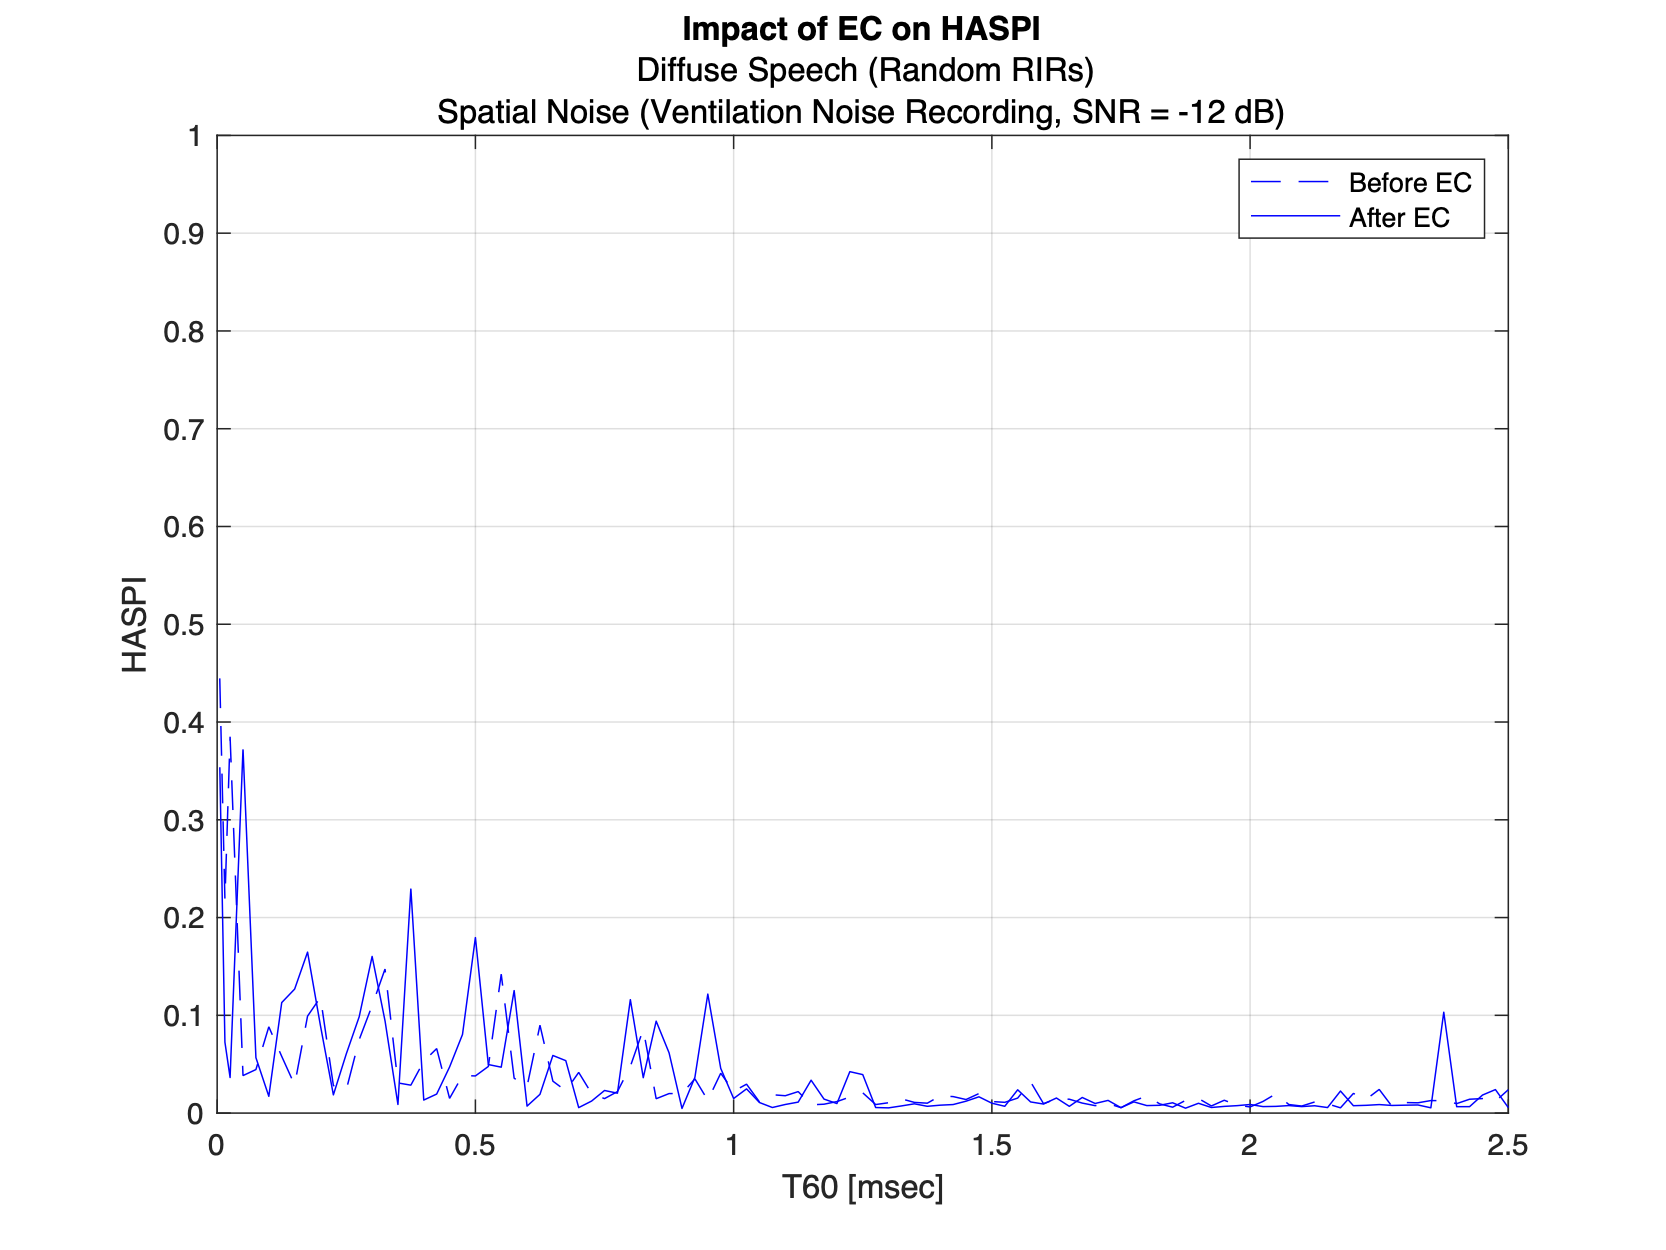
\includegraphics[width=\textwidth]{EC_SRM_T60_SNRm12}
	\end{subfigure}
	\hfill
	\begin{subfigure}[b]{0.49\textwidth}
		\centering
		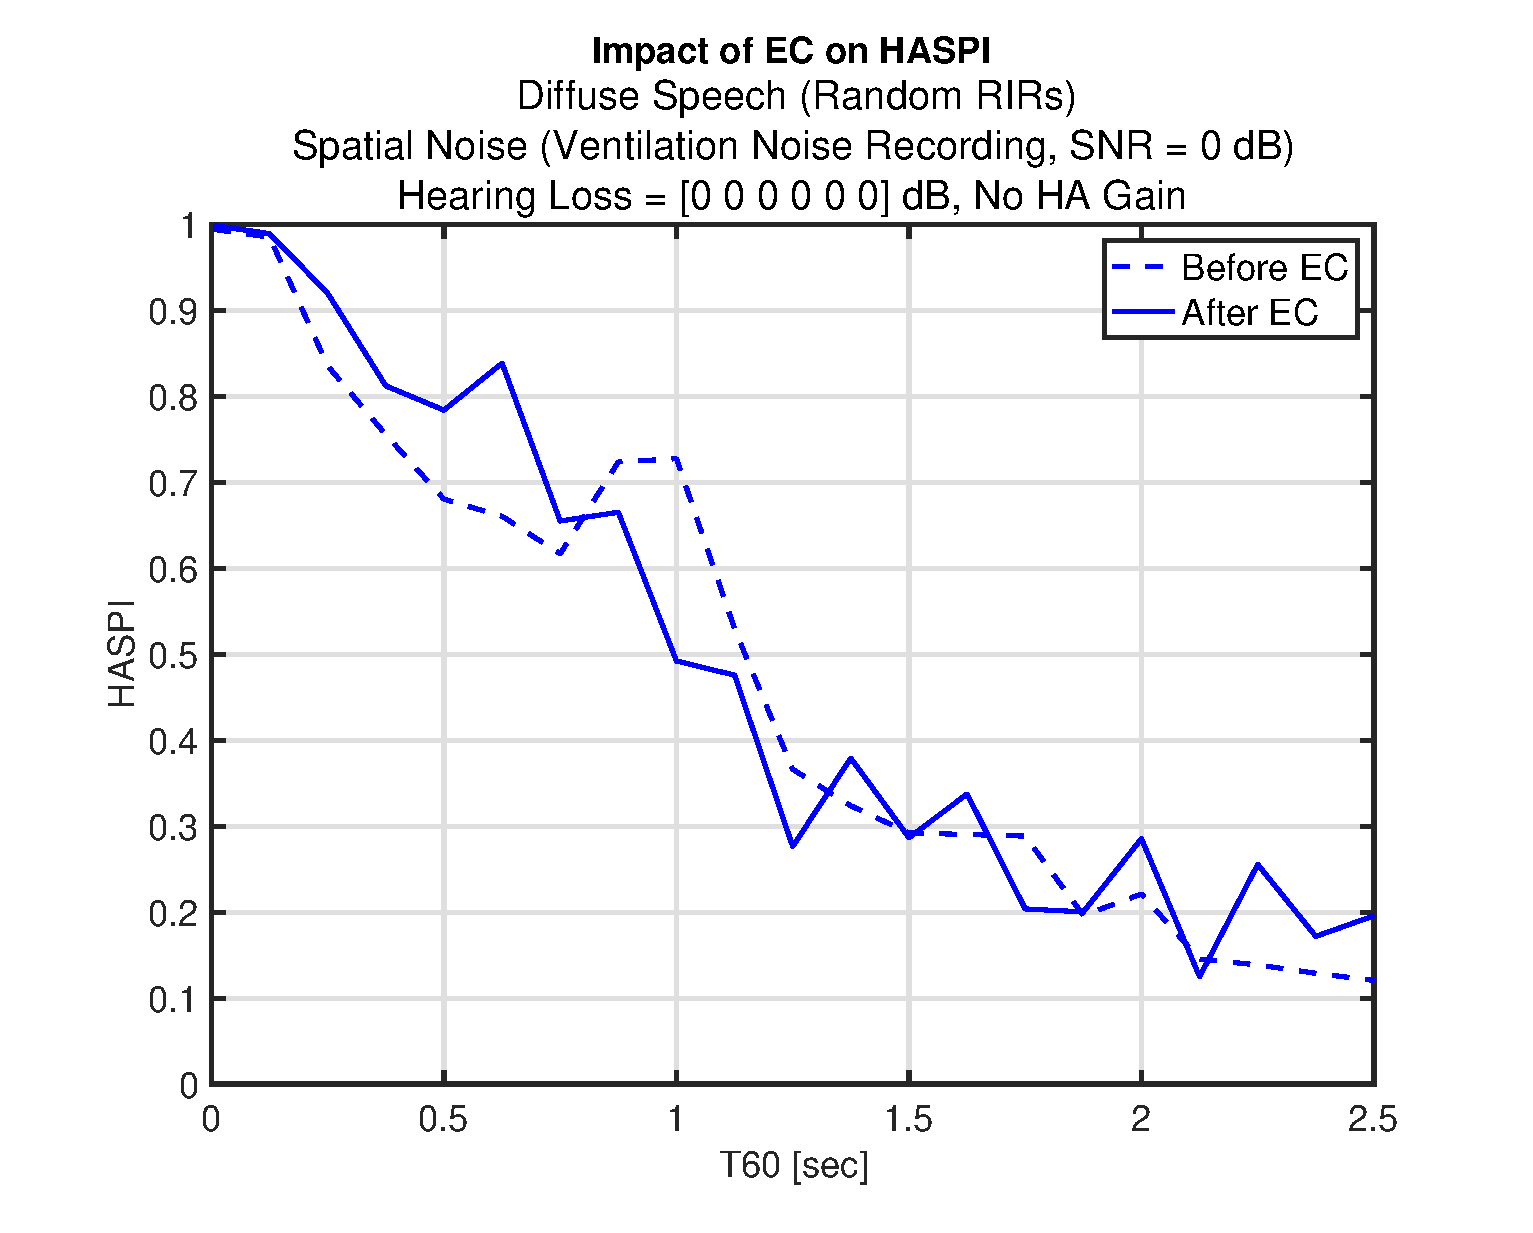
\includegraphics[width=\textwidth]{EC_SRM_T60_SNR0}
	\end{subfigure}
	\caption{Impact of EC algorithm on speech intelligibility (using HASPI) as a function of varying amounts of synthetic reverb, for spatial noise recording with SNR = \qty{-12}{\decibel} and SNR = \qty{0}{\decibel}}
	\label{fig:EC_SRM_T60}
\end{figure}

- Diffuse reverb destroys binaural cues and reduces the binaural benefit modeled by the EC (this provides modeling of the reduction in SRM due to reverb). However at low T60s the RIR is less diffuse and therefore can randomly have more emphasized directions thus sometimes providing some binaural benefit
- Note distinction between SRM for noise and reverb (EC models reduction in SRM due to reverb, but doesnt model reduction in reverb itself)

- SNR = 0 dB: SI is already saturated, so only evaluating impact of reverb (essentially SNR = infinity)

\textbf{Does EC capture any of the benefits of early reflections?}


\begin{figure}[H]
	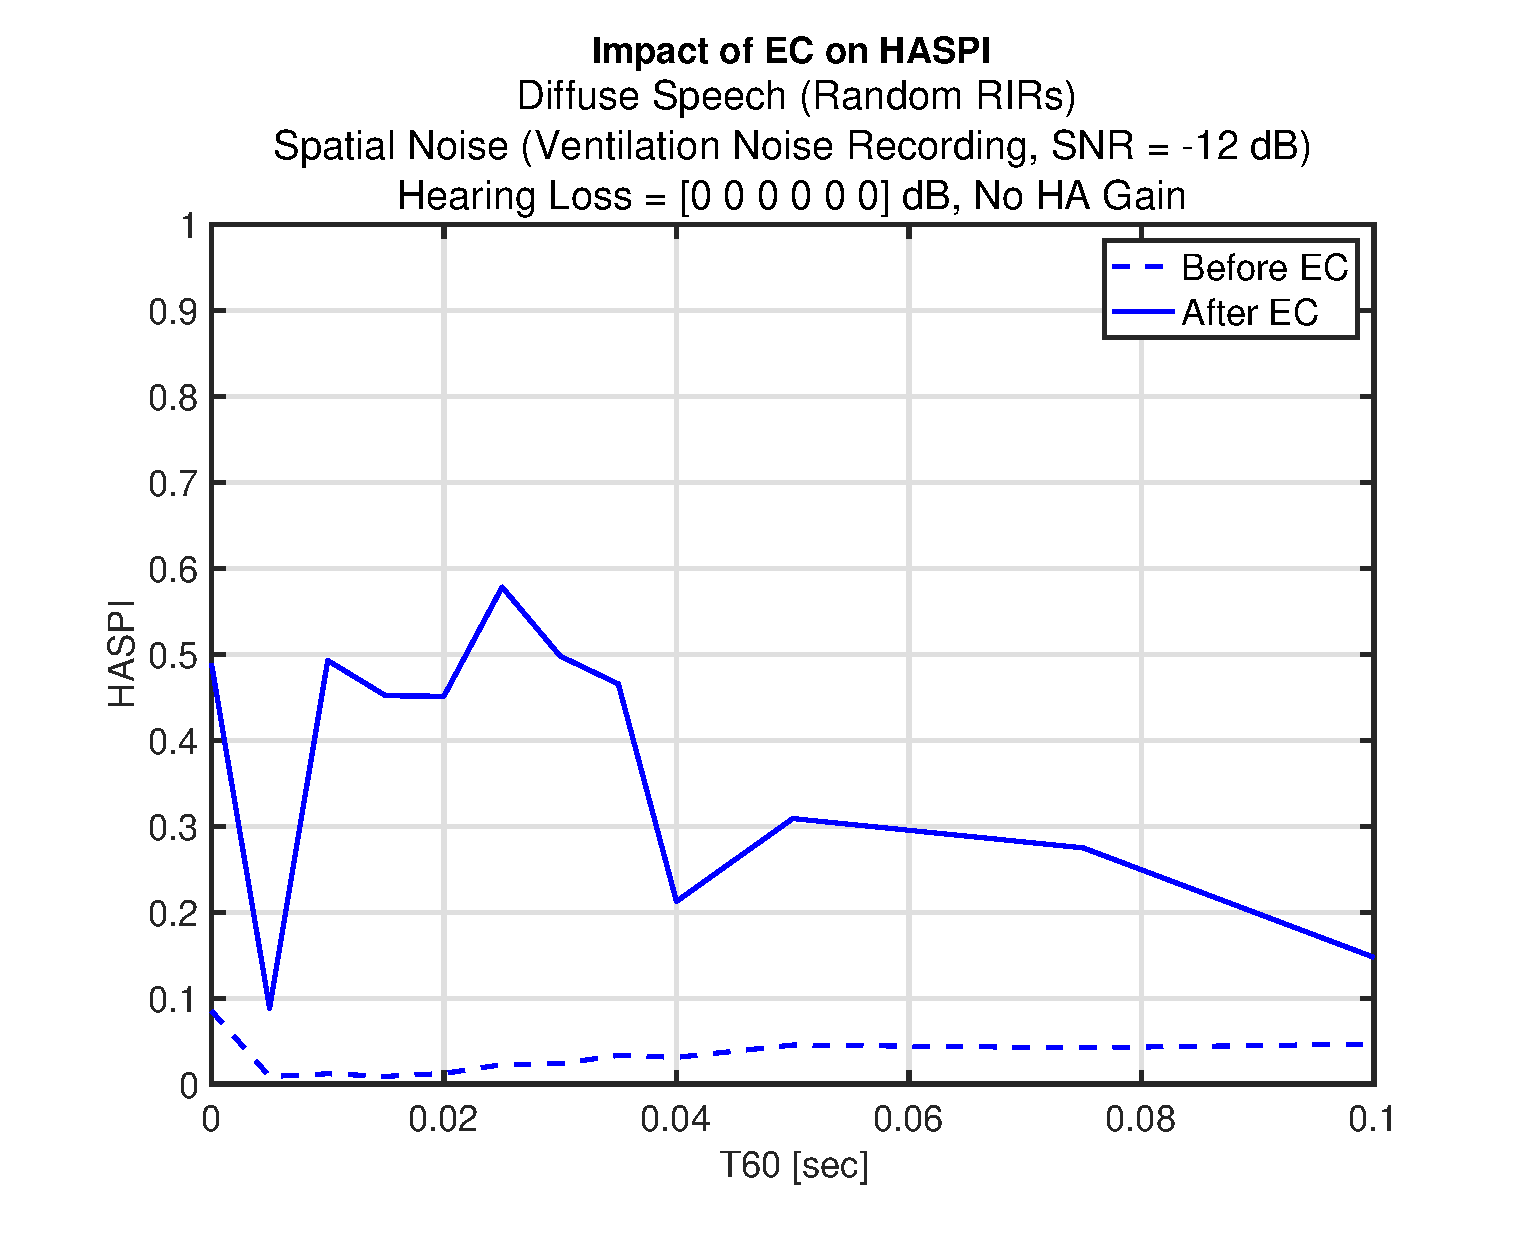
\includegraphics[width=0.7\textwidth]{EC_ERs}
	\centering
	\caption{Impact of EC algorithm on speech intelligibility (using HASPI) as a function of varying amounts of synthetic reverb, for spatial noise recording with SNR = \qty{-12}{\decibel}  }
	\label{fig:EC_ReverbSNRBoost}
\end{figure}

- Diffuse reverb (white noise) used to focus on temporal integration rather than spatial separation -- Most significant binaural benefit for T60 = 0 (no benefit of early reflections) -- However repeating the experiment several times reveals occasional benefit depending on the randomly generated RIR -- assumed this is just due to sometimese the very short number of simulated reflections effectively coming from similar directions thus providing SRM

- I would expect that using real RIRs would result in some SRM from early reflections (since they tend not to be diffuse)

- Essentially all this shows that EC may provide some modeling of BINAURAL benefit of reverb in low SNR environments (SRM), but no modeling of MONAURAL benefit of reverb (PE temporal integration)


\textbf{EC on reverb only}

\begin{figure}[H]
	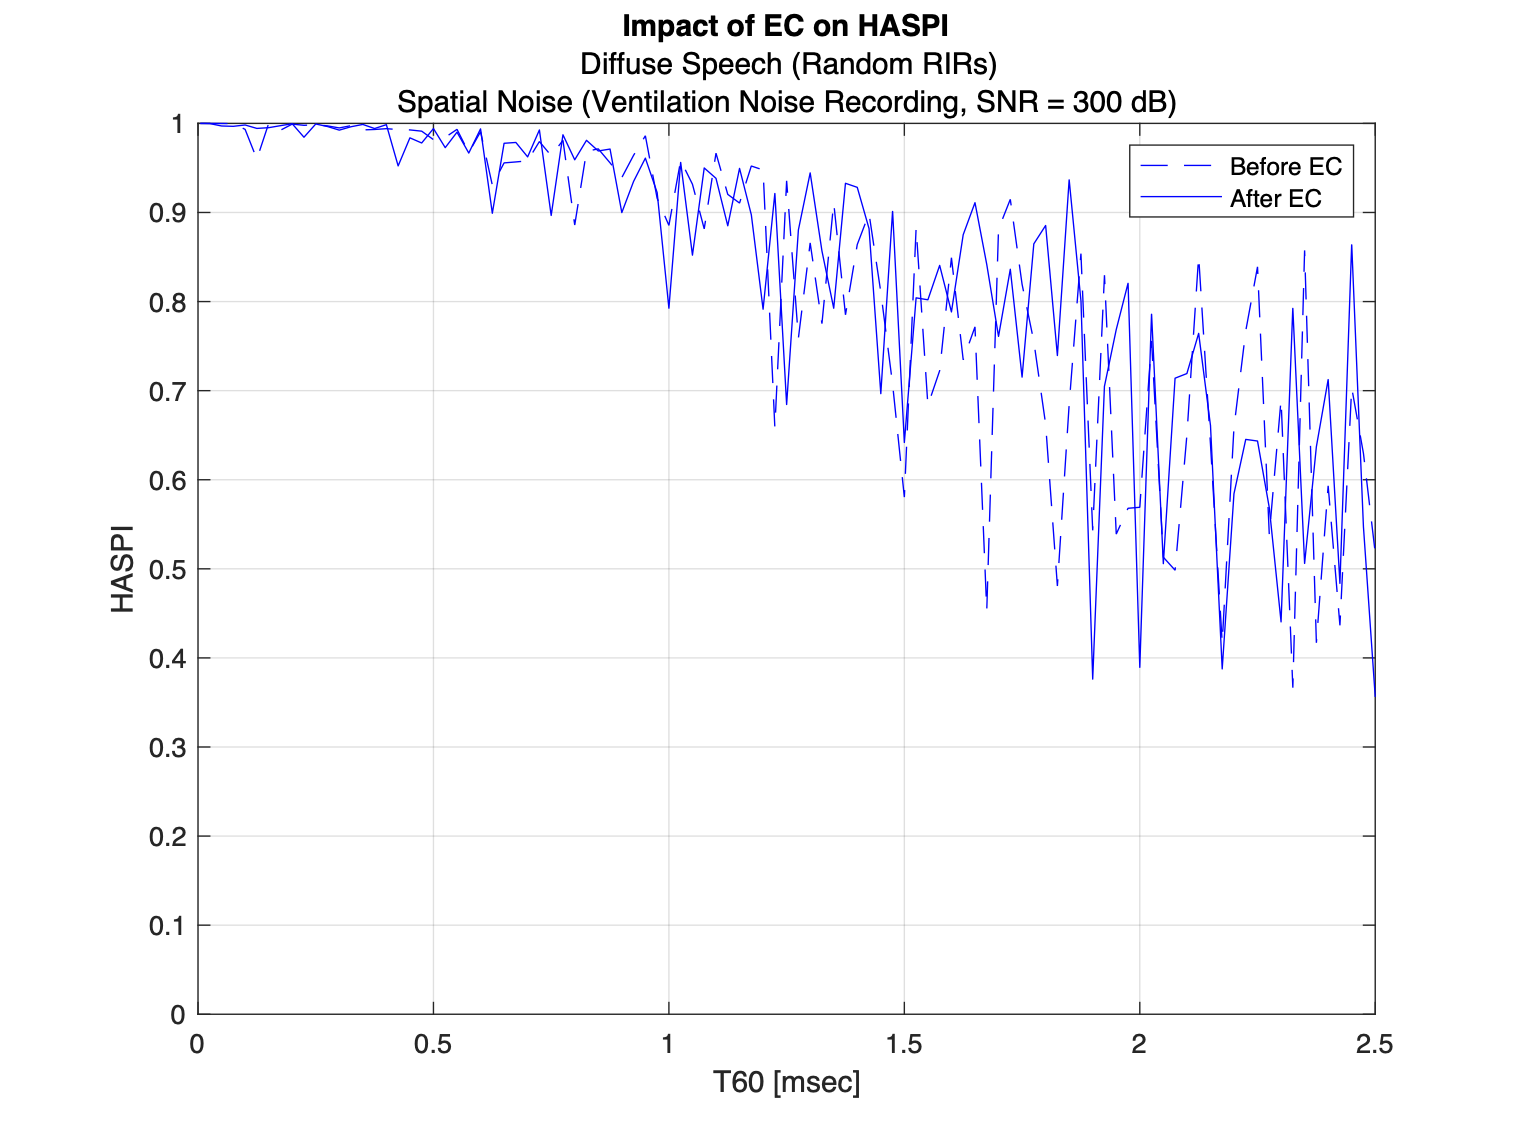
\includegraphics[width=0.7\textwidth]{EC_SRM_T60_SNR300}
	\centering
	\caption{Impact of EC algorithm on speech intelligibility (using HASPI) as a function of varying amounts of synthetic reverb, noise-free}
	\label{fig:EC_SRM_T60_SNR300}
\end{figure}

- EC does not provide binaural benefit in reverb

- EC focuses on canceling interfering noise from certain directions, which doesnt apply to reducing reverb since (for high T60s) reverb tends towards diffuse, and the interfering reflections are correlated to the clean speech



\subsection{Hearing Aid Gain Comparison}

Ian:

- Loudness recruitment and its influence on WDRC design (Threshold of hearing increasing doesnt increase in upper limit where loudness becomes too much -- reduced dynamic range)

- Question: Do nonlinearities in auditory system still apply at same higher SPL with hearing loss? If so then this is another reason for not doing mirror audiogram compensation (not just comfort, but going to these high levels will distort cues making SI worse -- Shouldnt this be picked up by the metrics?)

- Look at Hearing Aid textbook from Harvey Dillon

- NAL-R ideal at conversational speech, quieter you want closer to mirror audiogram, and louder sounds you want less than NAL-R

- Generally speaking in terms of restoring the representation (maybe also in STMI/NSIM -- pretty sure Ian knows but im missing something) mirror audiogram will be optimal for SI, NAL-R is more about comfort -- We cant do mirror audiogram because users wont like it, NAL-R is better in terms of trade off of SI and comfort

\begin{figure}[H]
	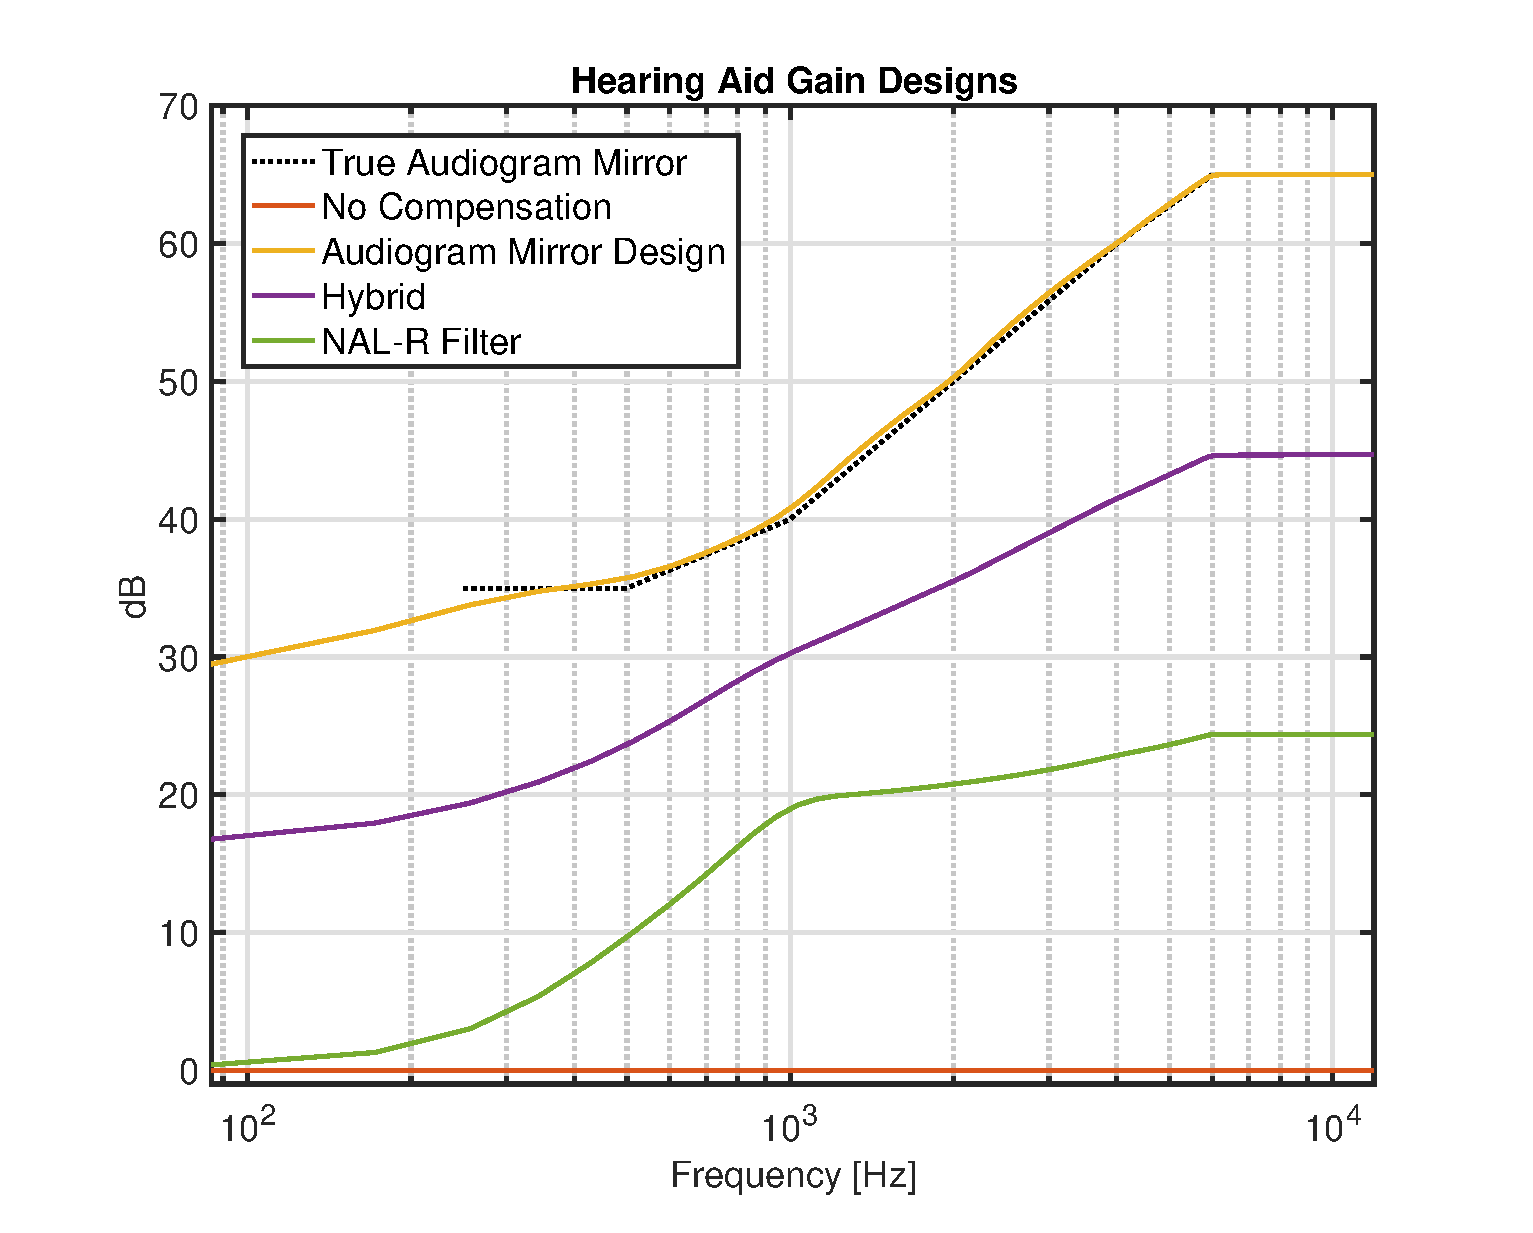
\includegraphics[width=0.7\textwidth]{HearingAidGains}
	\centering
	\caption{Hearing aid gains to be used in evaluation}
	\label{fig:HA_Gains}
\end{figure}

\begin{figure}[H]
	\centering
	\begin{subfigure}[b]{0.49\textwidth}
		\centering
		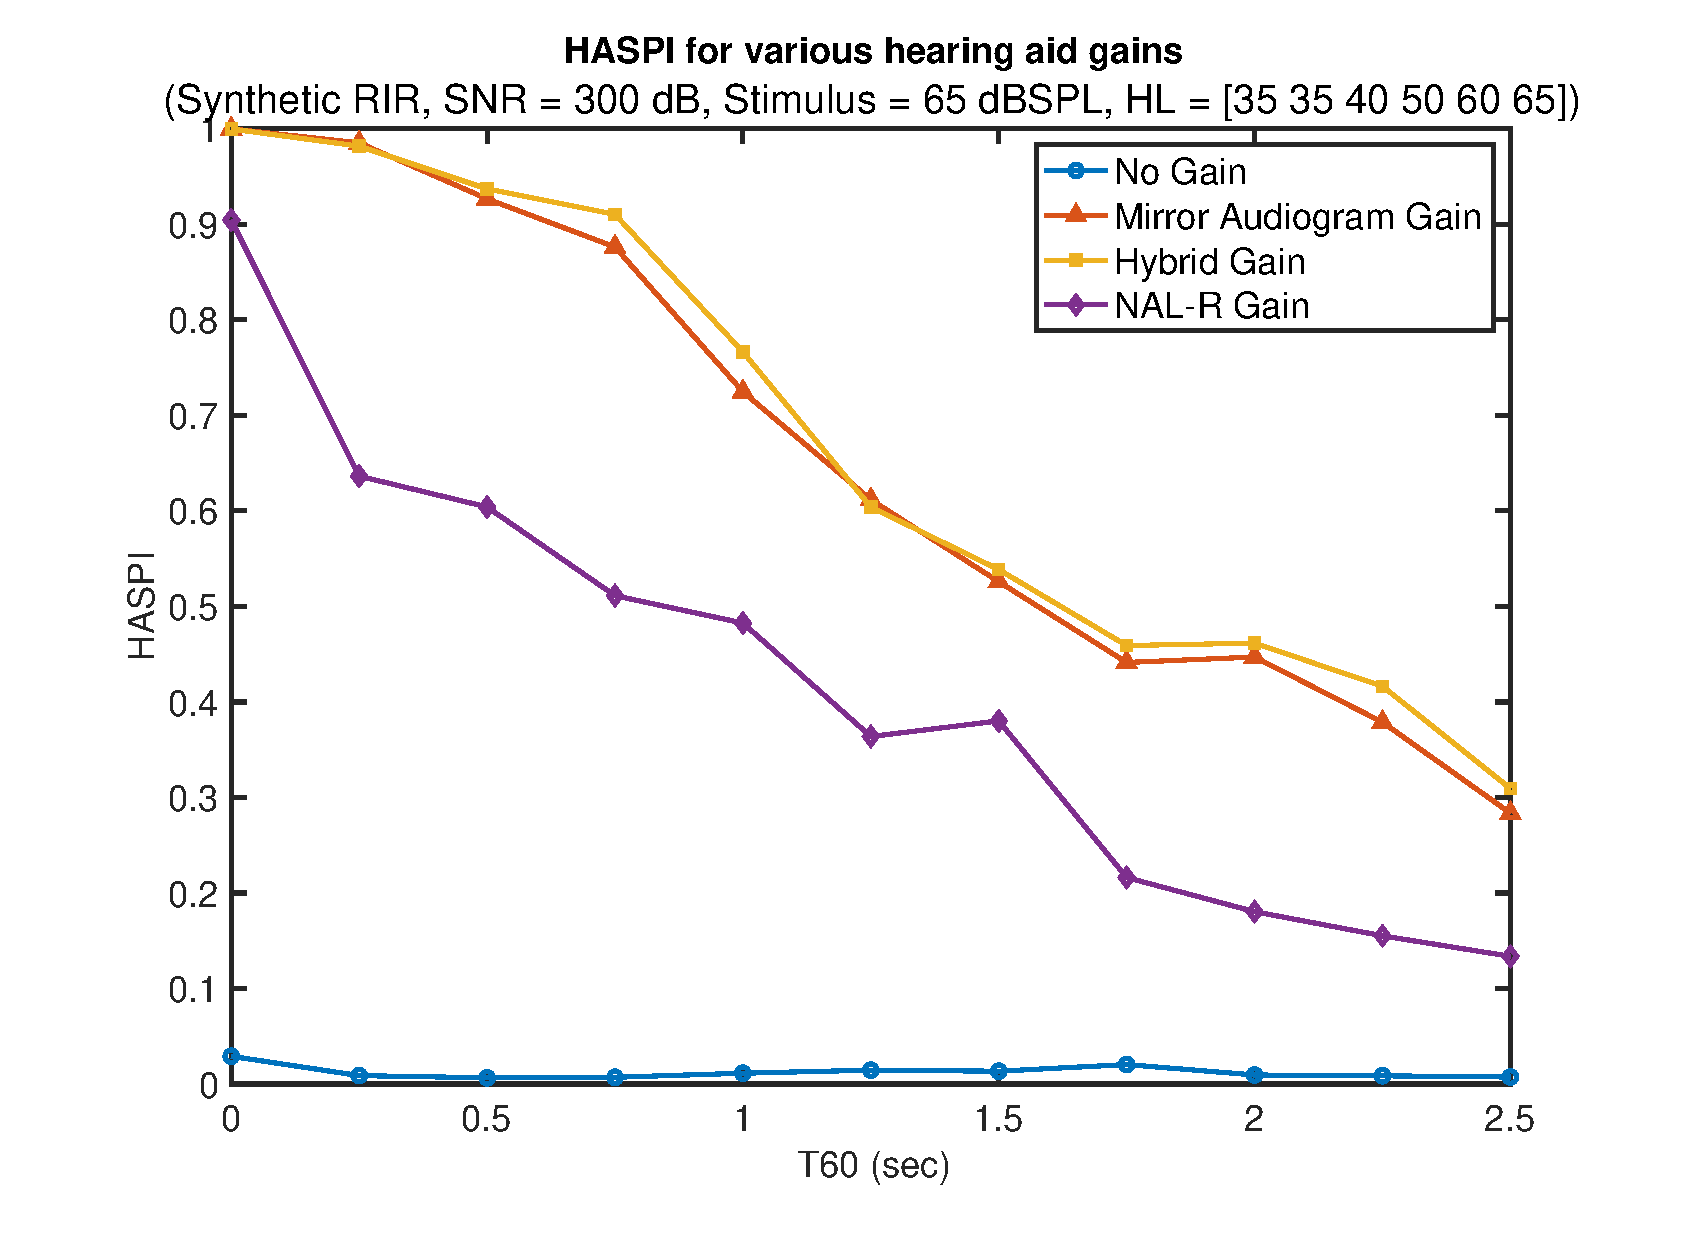
\includegraphics[width=\textwidth]{HASPI_v_T60_variousHAGains}
	\end{subfigure}
	\hfill
	\begin{subfigure}[b]{0.49\textwidth}
		\centering
		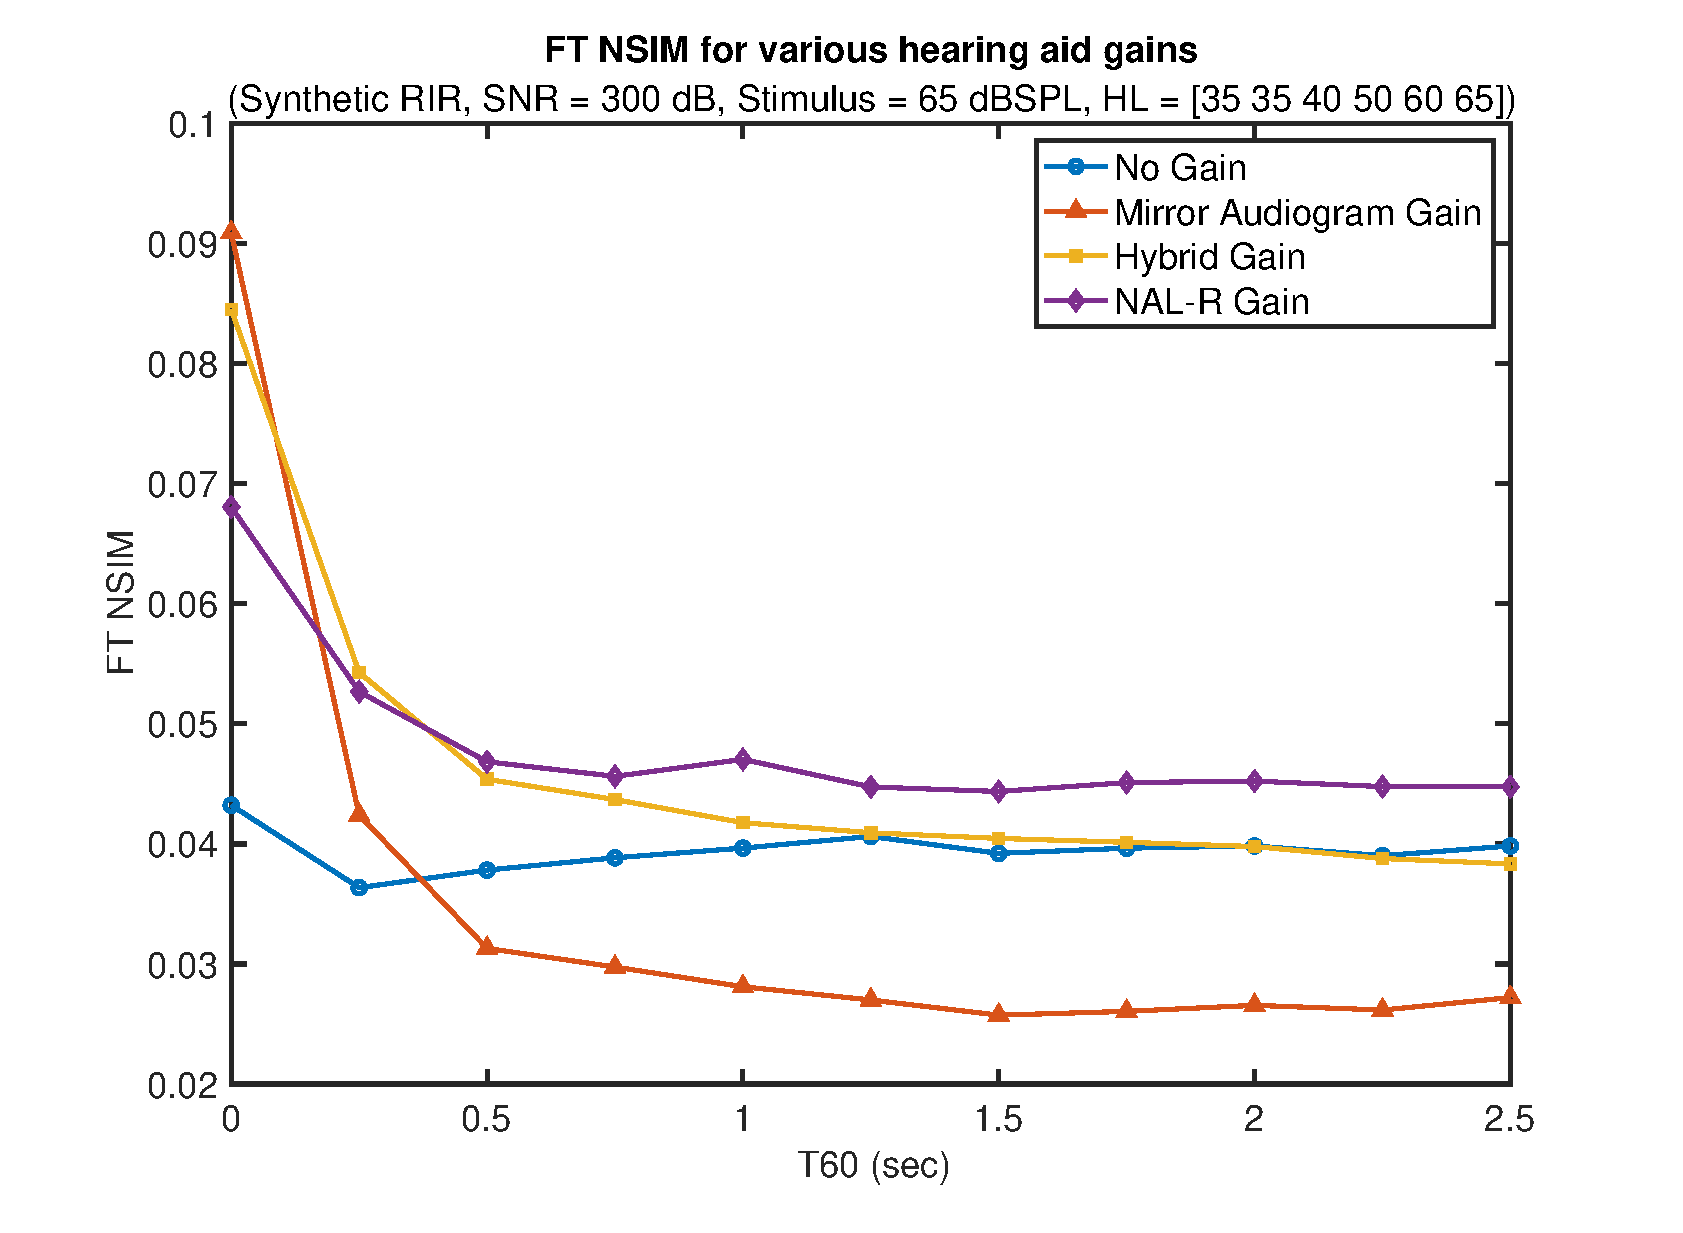
\includegraphics[width=\textwidth]{NSIM_FT_v_T60_variousHAGains}
	\end{subfigure}
	\hfill
	\begin{subfigure}[b]{0.49\textwidth}
		\centering
		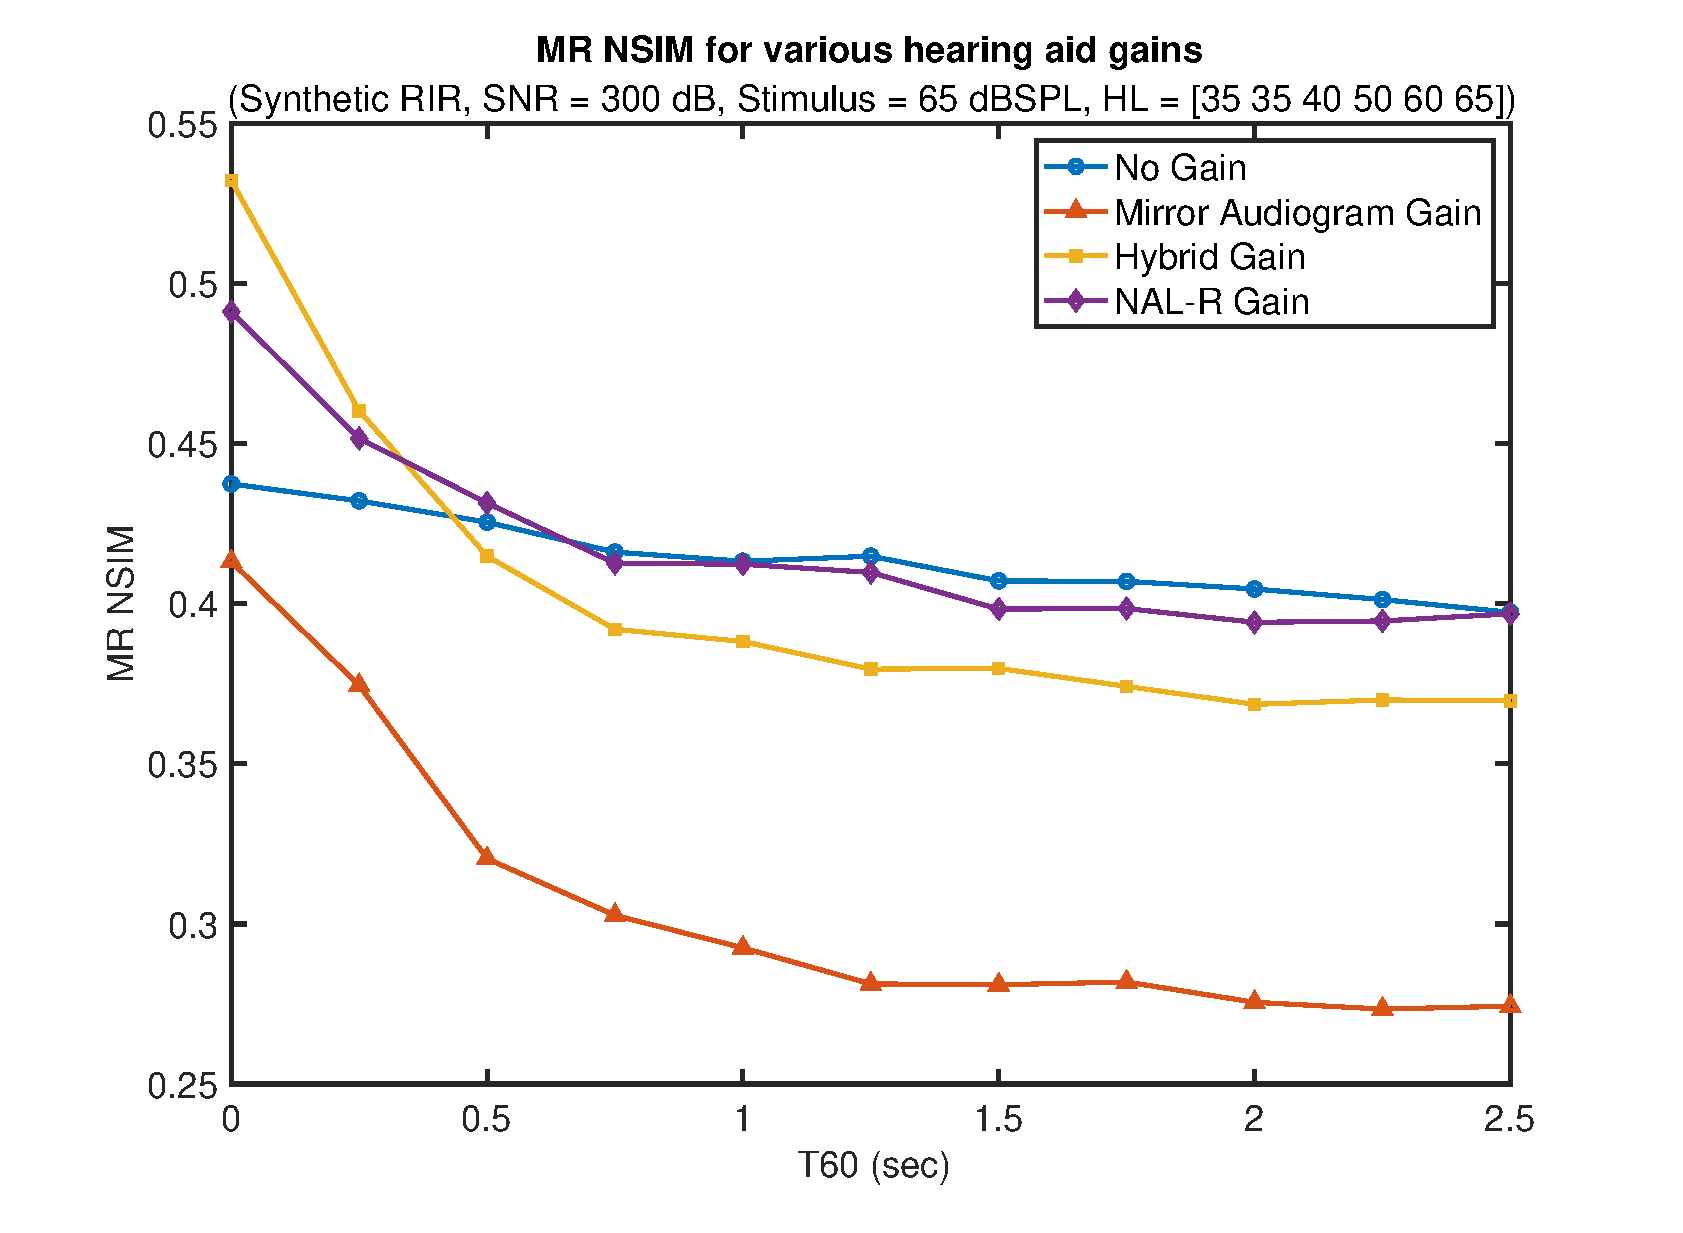
\includegraphics[width=\textwidth]{NSIM_MR_v_T60_variousHAGains}
	\end{subfigure}
	\hfill
	\begin{subfigure}[b]{0.49\textwidth}
		\centering
		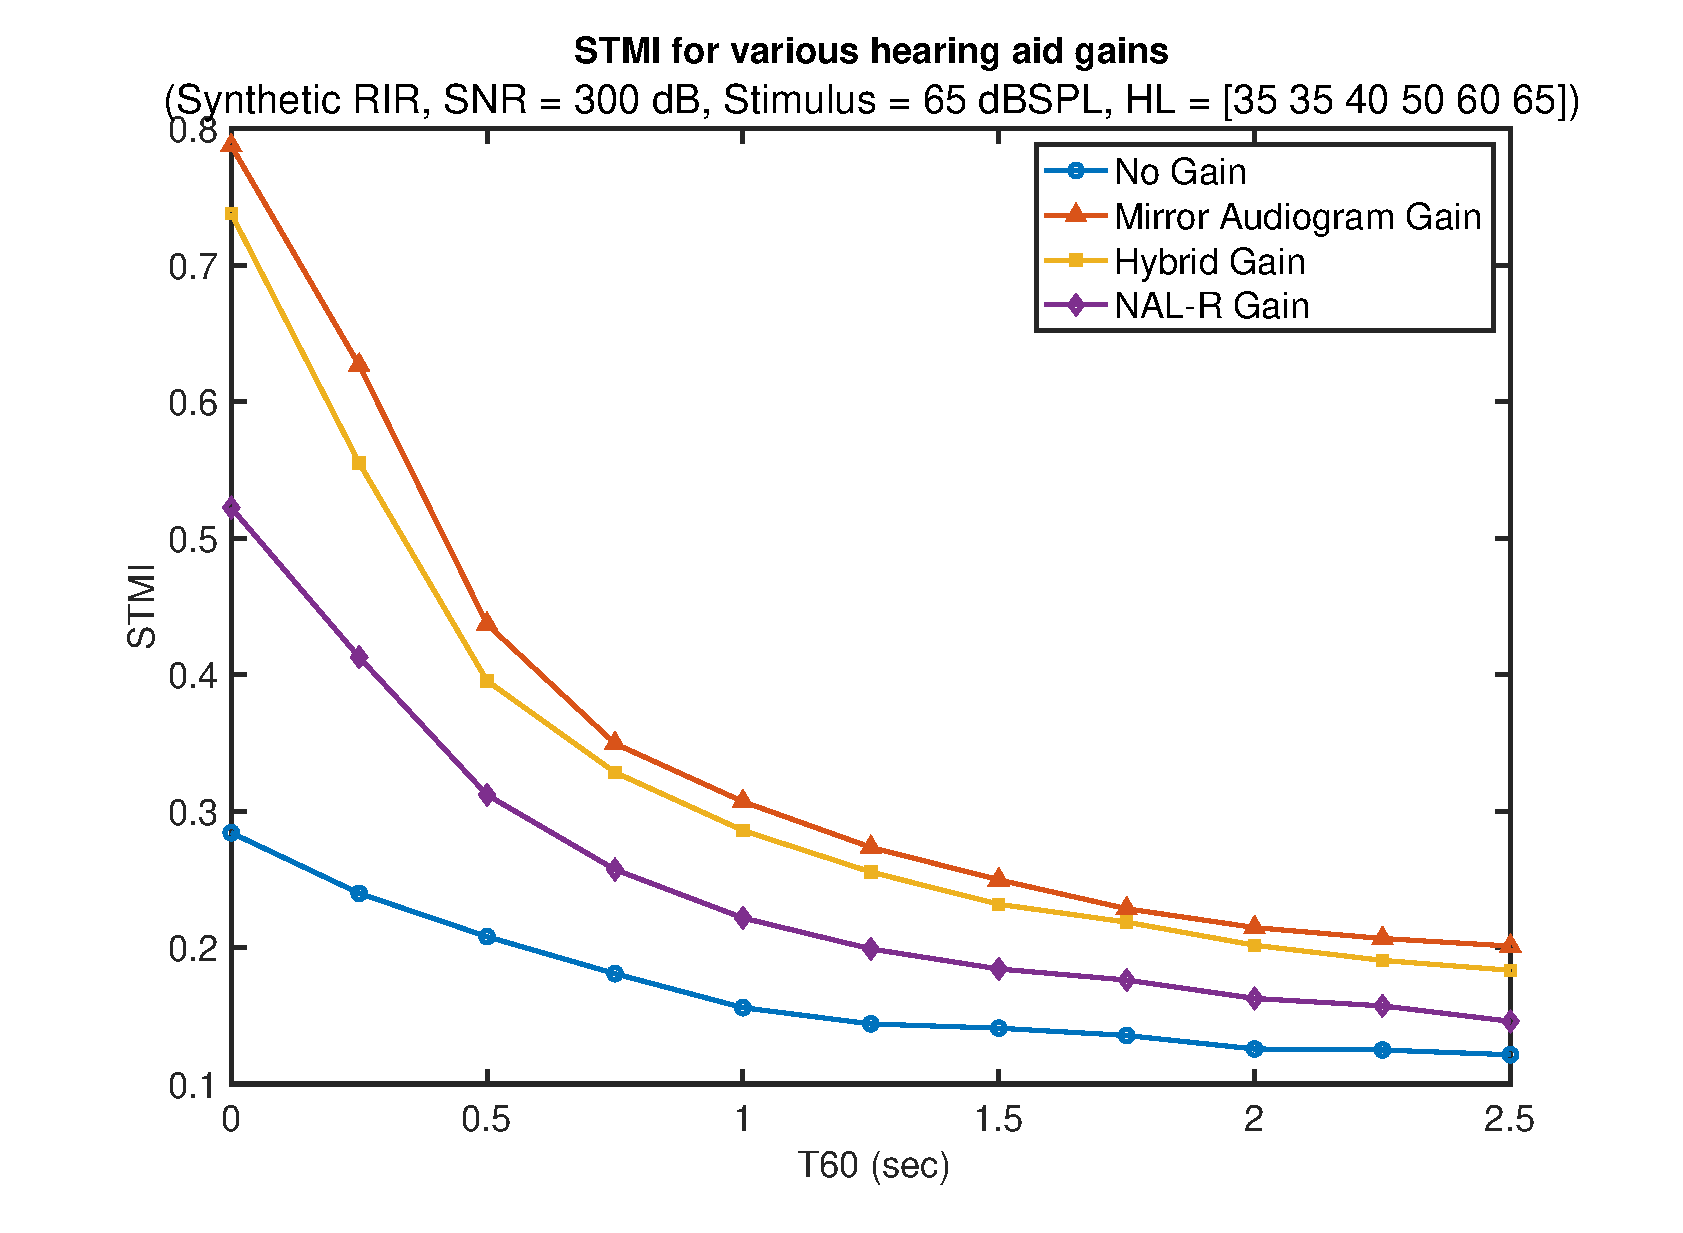
\includegraphics[width=\textwidth]{STMI_v_T60_variousHAGains}
	\end{subfigure}
	\hfill
	\caption{Comparison of perceptual benefit of four different linear hearing aid gains in the presence of reverb. Moderate high frequency hearing loss used in the perceptual models (IEC 60118-15 Moderate HL, Moderately Sloping Group), and RIRs were generated synthetically}
	\label{fig:HA_GainComparison}
\end{figure}



\subsection{Evaluation of Monaural Speech Intelligibility Metrics In Context of Reverberation}


\begin{figure}[H]
	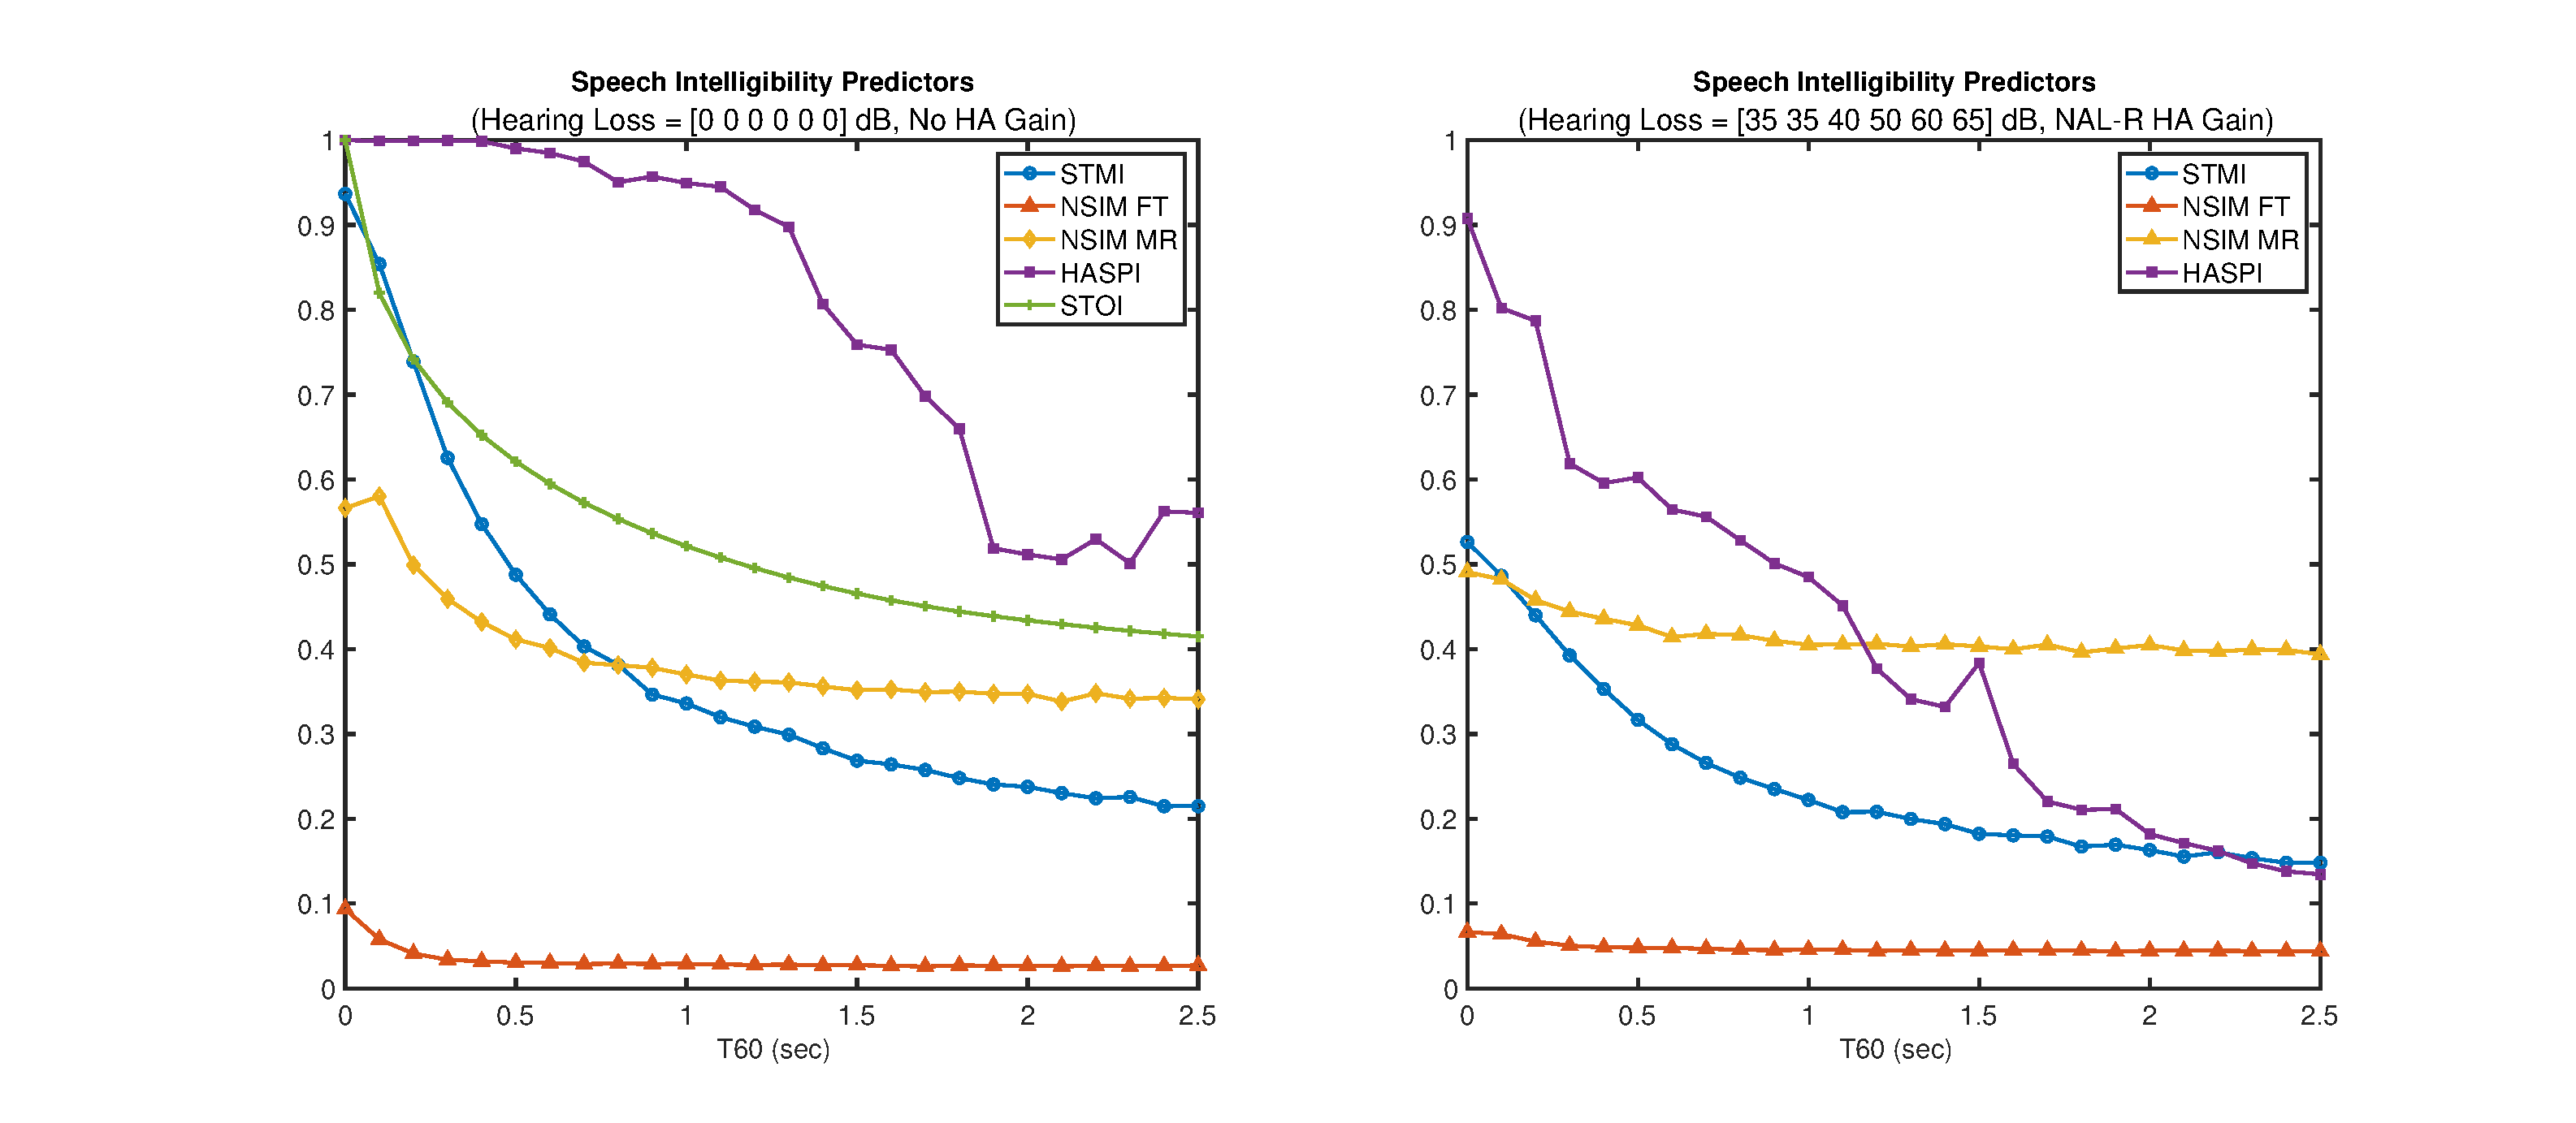
\includegraphics[width=0.98\textwidth]{SIMetricsEval_Synthetic}
	\centering
	\caption{Impact of synthetic reverberation (exponentially decaying gaussian RIRs) on SI predictors with and without hearing loss. NAL-R linear hearing aid amplification included in hearing loss case for metrics that including modeling of hearing loss}
	\label{fig:SIMetricsEval_Synthetic}
\end{figure}

\begin{figure}[H]
	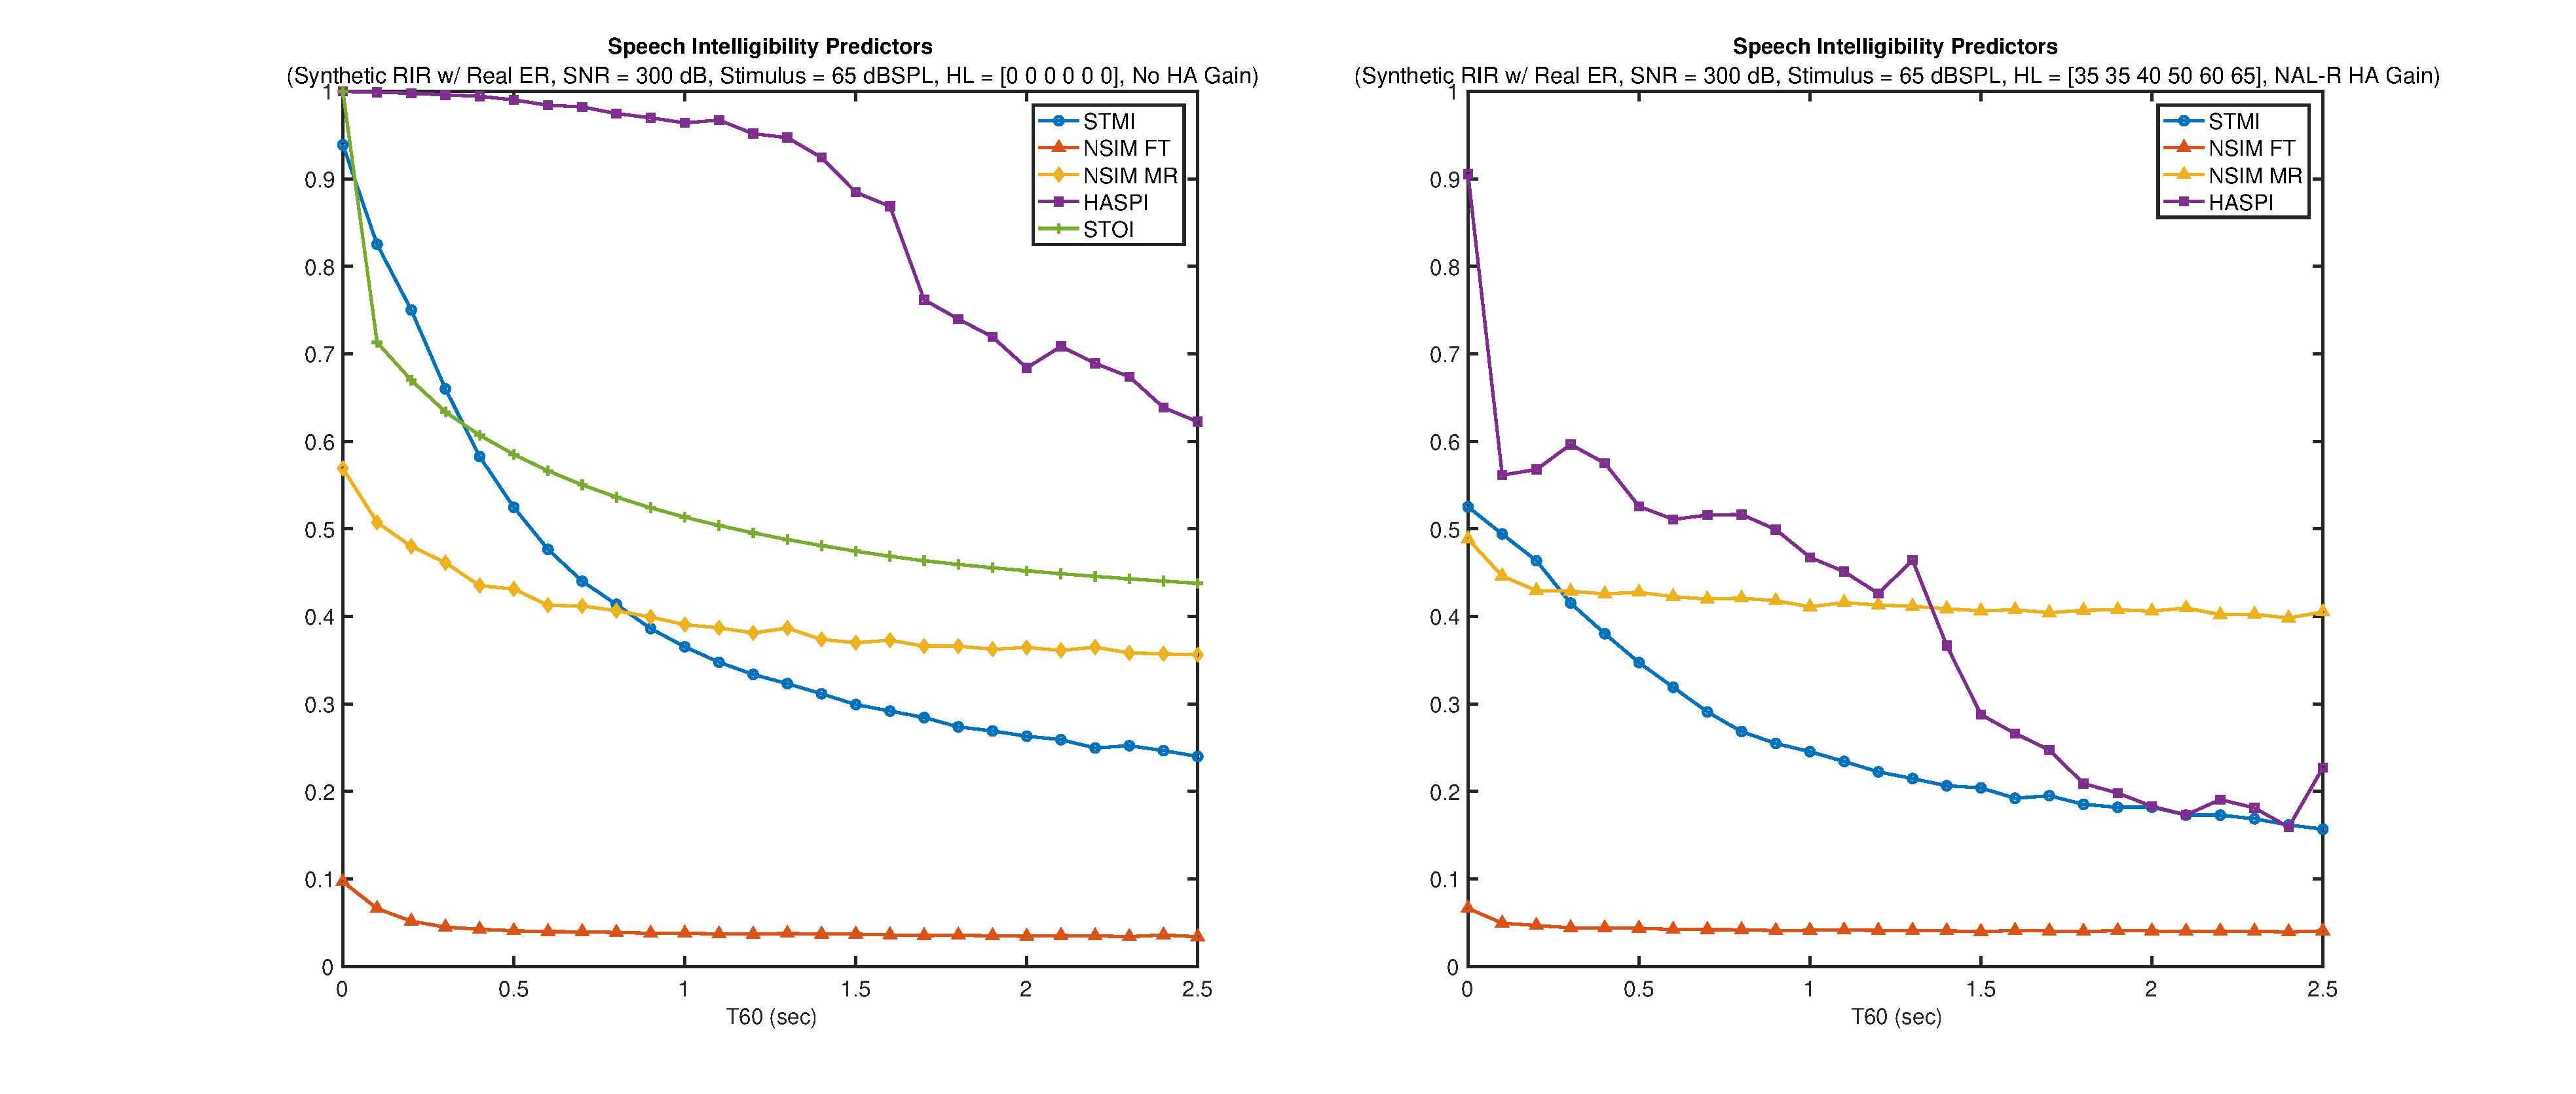
\includegraphics[width=0.98\textwidth]{SIMetricsEval_Synthetic_RealER}
	\centering
	\caption{Impact of synthetic reverberation (exponentially decaying gaussian RIRs) with added real early reflections generated by truncating a real RIR  (Office II RIR from the HRIR database) on SI predictors with and without hearing loss. NAL-R linear hearing aid amplification included in hearing loss case for metrics that including modeling of hearing loss}
	\label{fig:SIMetricsEval_Synthetic_RealER}
\end{figure}

\begin{figure}[H]
	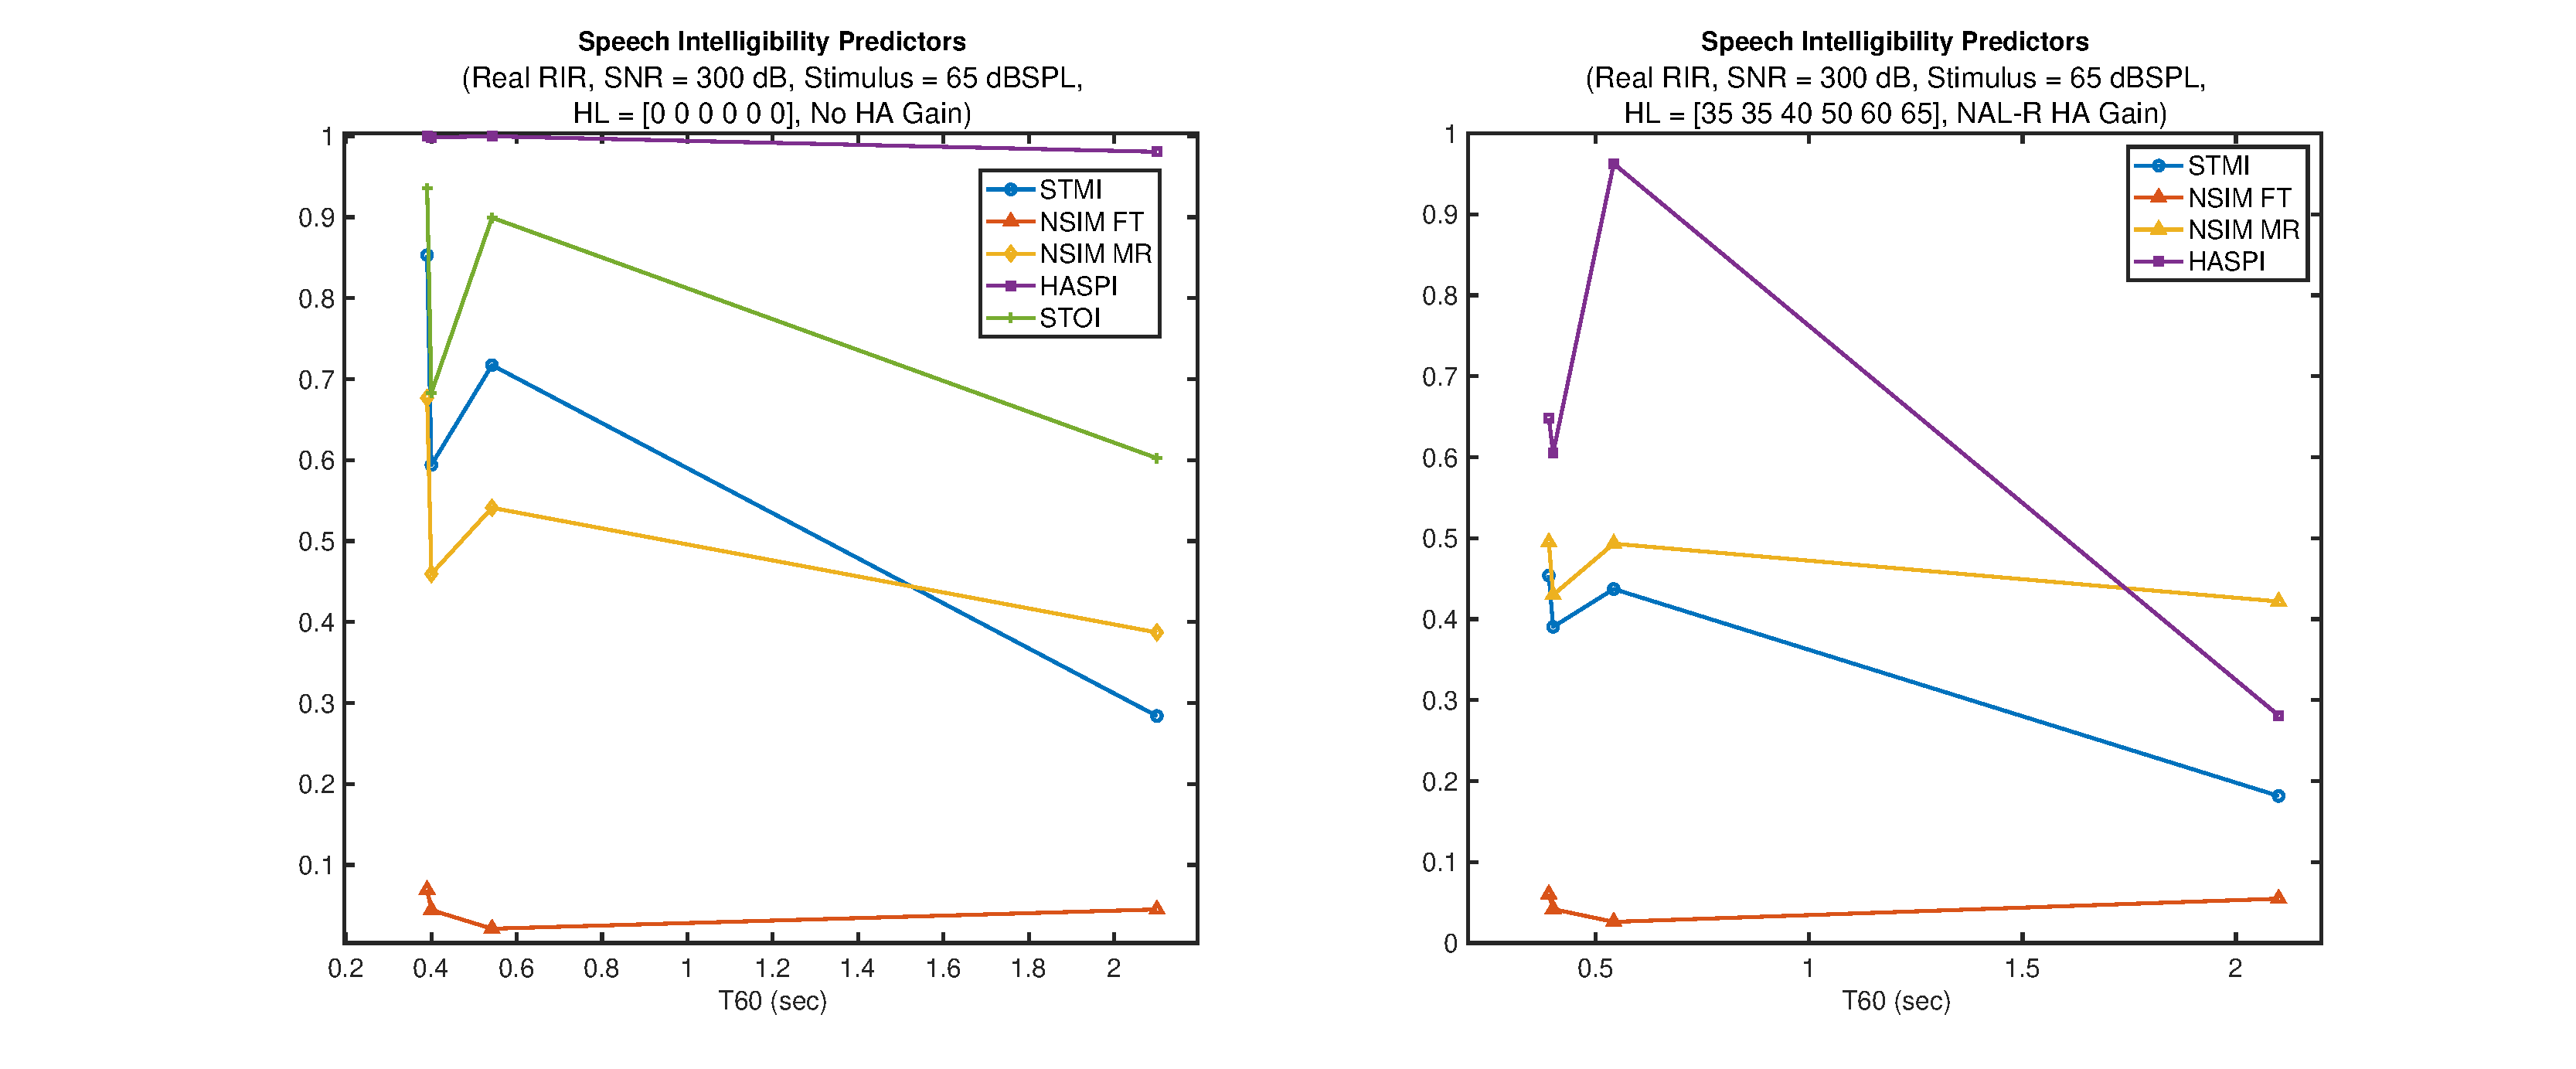
\includegraphics[width=0.98\textwidth]{SIMetricsEval_Real}
	\centering
	\caption{Impact of practical reverberation (several real measured RIRs) on SI predictors with and without hearing loss. NAL-R linear hearing aid amplification included in hearing loss case for metrics that including modeling of hearing loss}
	\label{fig:SIMetricsEval_Real}
\end{figure}

- Discussion of how SAL was truncated synthetically to control T60

\begin{figure}[H]
	\centering
	\begin{subfigure}[b]{0.49\textwidth}
		\centering
		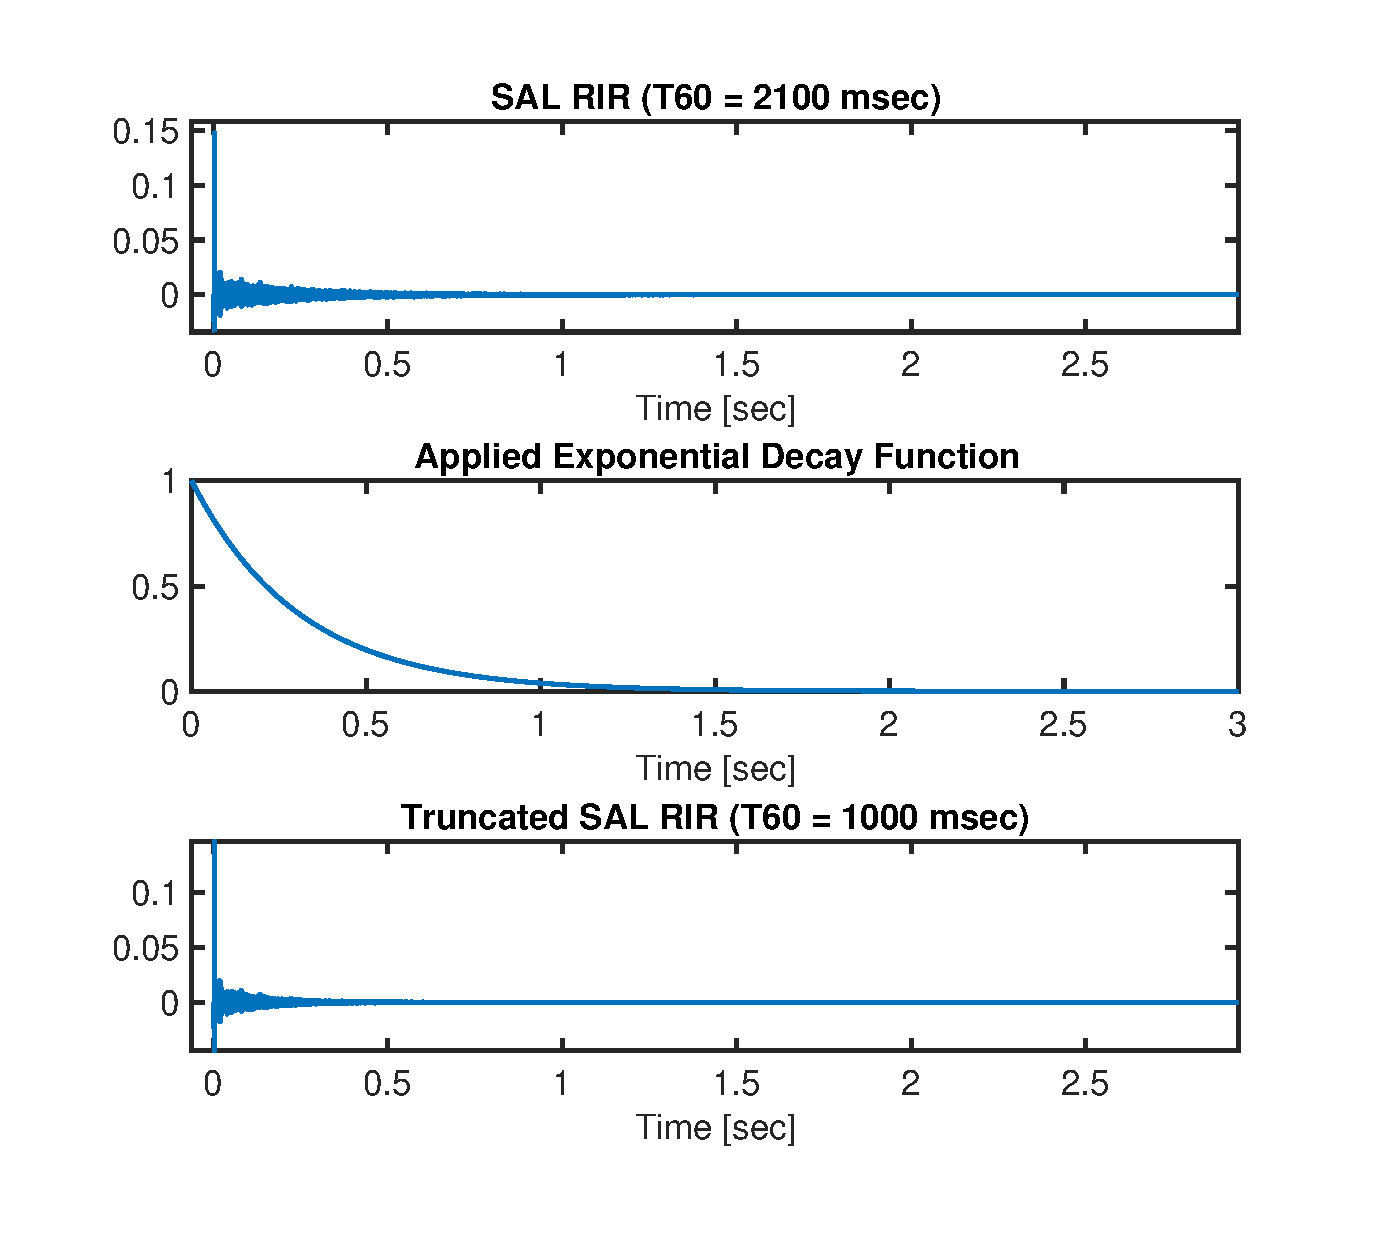
\includegraphics[width=\textwidth]{SALTruncationExample_RIR}
	\end{subfigure}
	\hfill
	\begin{subfigure}[b]{0.49\textwidth}
		\centering
		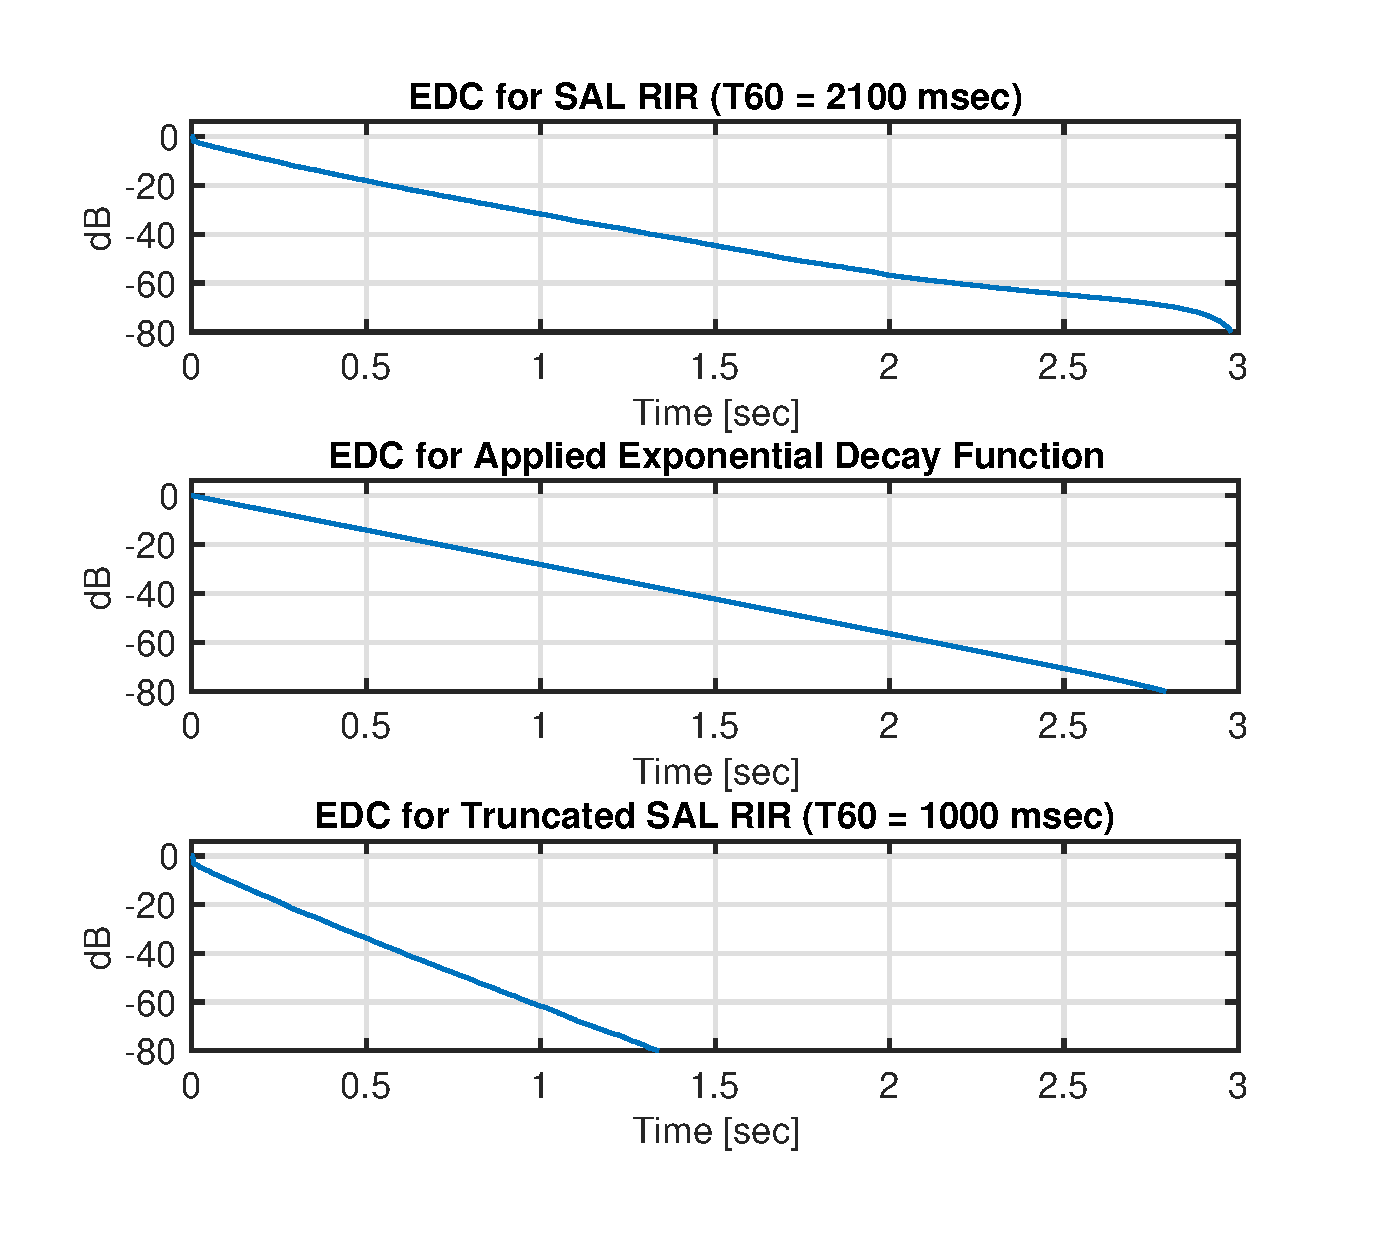
\includegraphics[width=\textwidth]{SALTruncationExample_EDC}
	\end{subfigure}
	\hfill
	\caption{TODO: REPLOT THIS WITH SAME X-AXIS USED IN ALL PLOTS FOR EDC. Example of how SAL was truncated by applying additional exponential decay as a window to manipulate T60 synthetically}
	\label{fig:SALTruncationExample}
\end{figure}

\begin{figure}[H]
	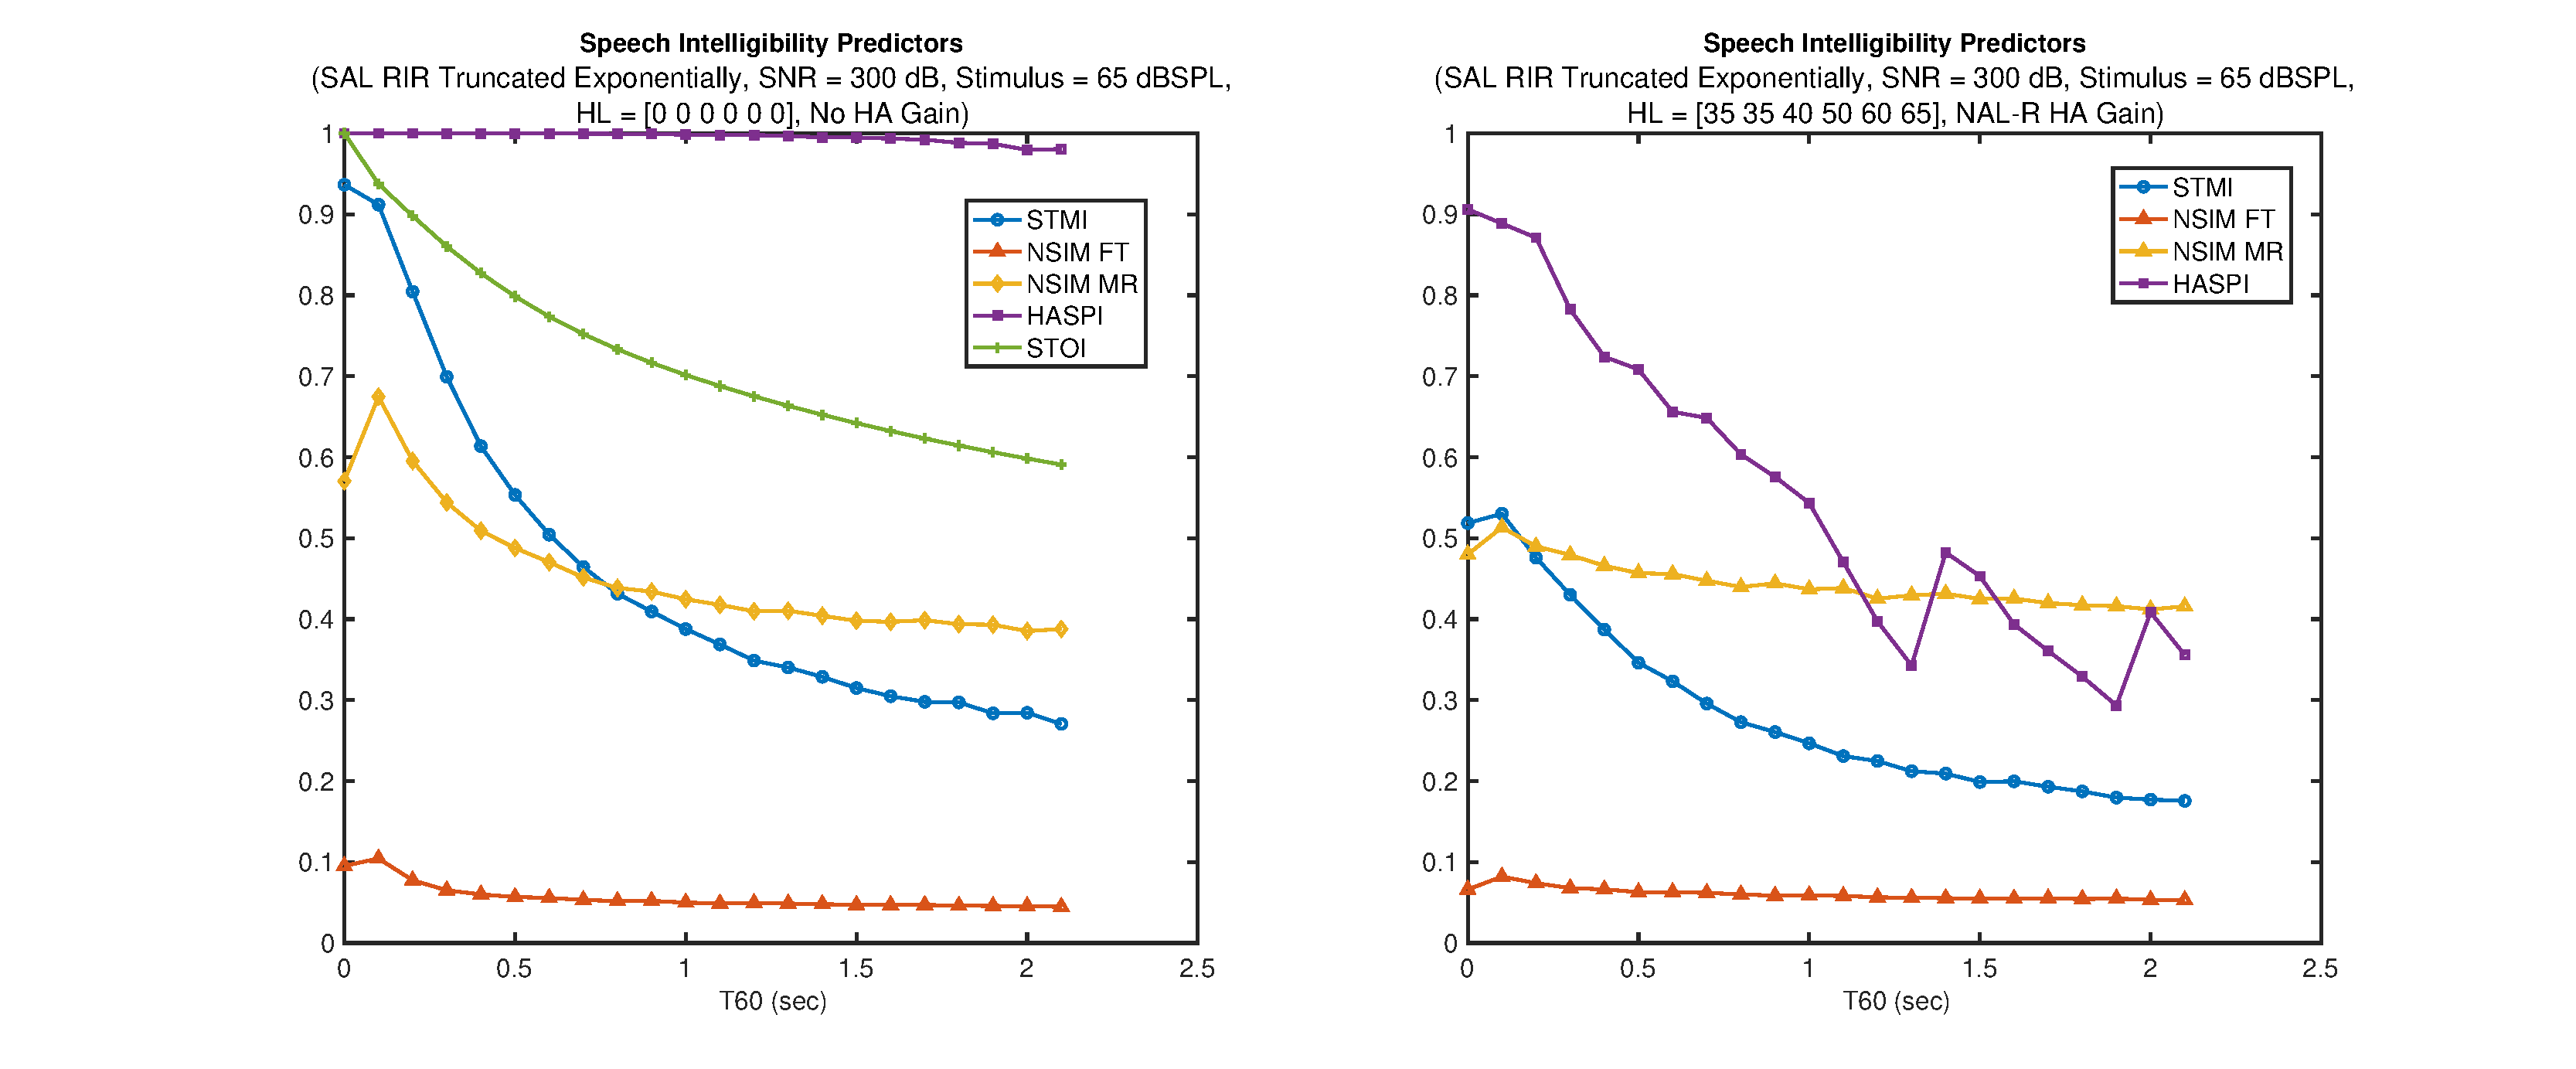
\includegraphics[width=0.98\textwidth]{SIMetricsEval_TruncatedSAL}
	\centering
	\caption{Impact of practical reverberation (SAL room from MYRiAD database exponentially truncated to control T60) on SI predictors with and without hearing loss. NAL-R linear hearing aid amplification included in hearing loss case for metrics that including modeling of hearing loss}
	\label{fig:SIMetricsEval_TruncatedSAL}
\end{figure}

- Discussion of how ER of SAL were reduced to make reverberation effect stronger


\begin{figure}[H]
	\centering
	\begin{subfigure}[b]{0.49\textwidth}
		\centering
		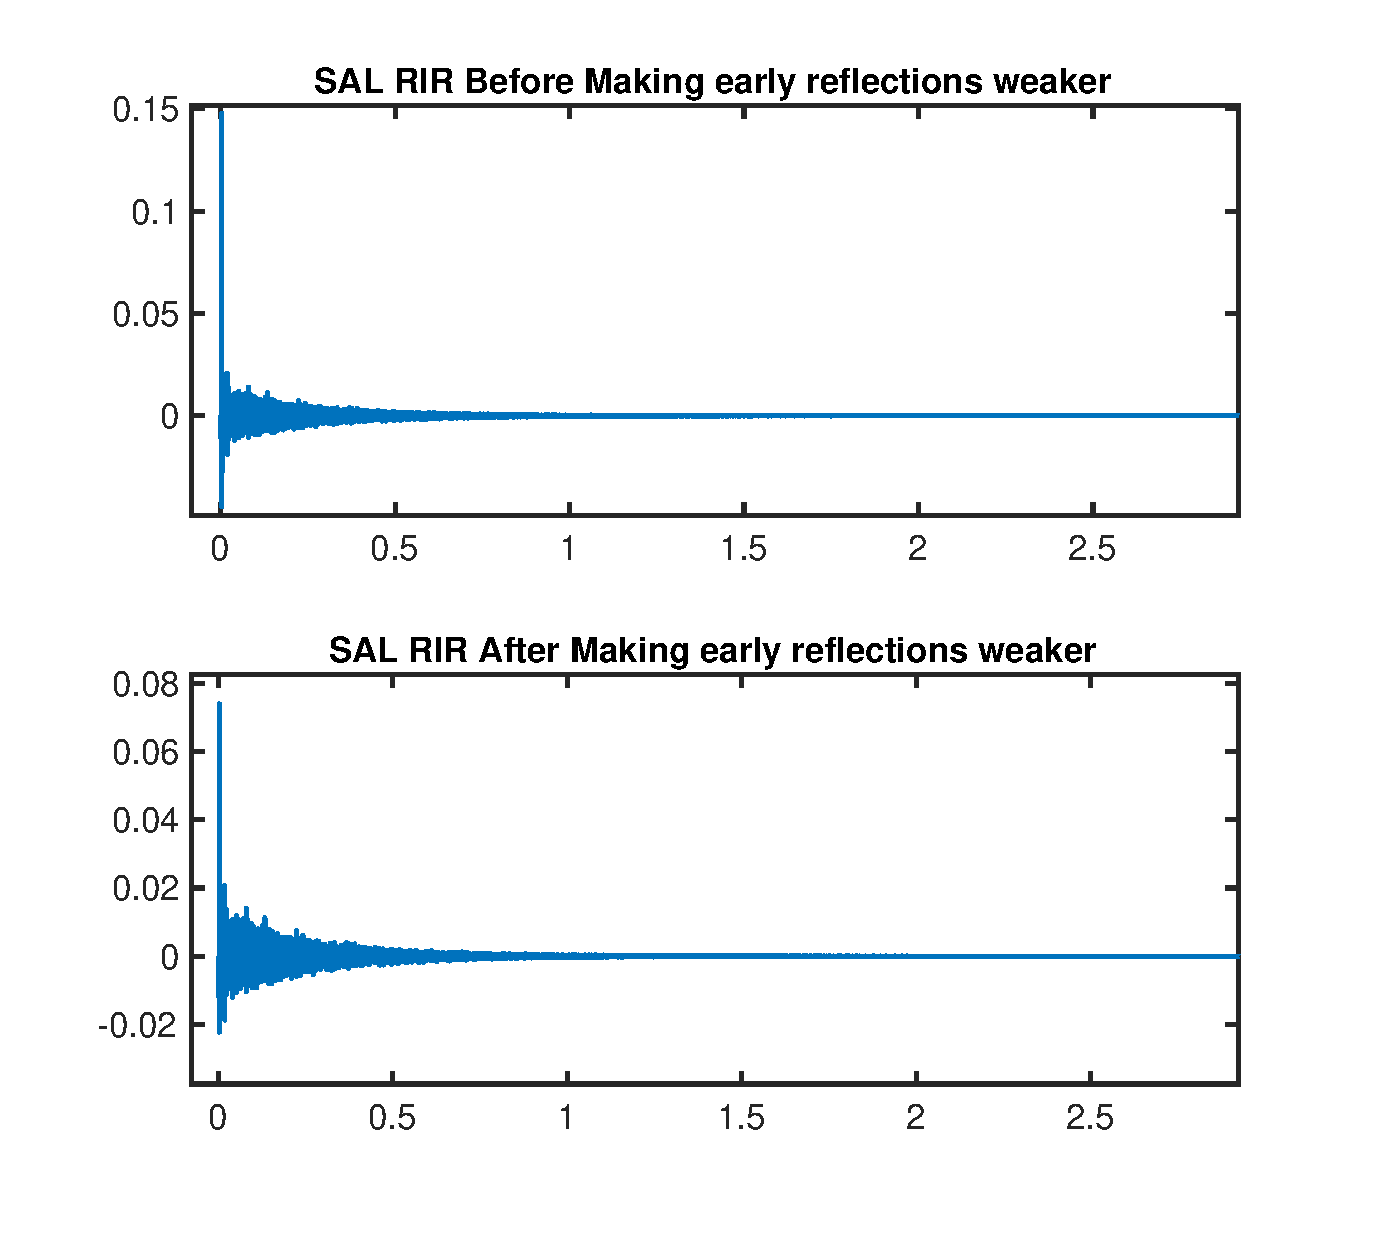
\includegraphics[width=\textwidth]{SAL_ERProcessingExample_Div2_RIR}
	\end{subfigure}
	\hfill
	\begin{subfigure}[b]{0.49\textwidth}
		\centering
		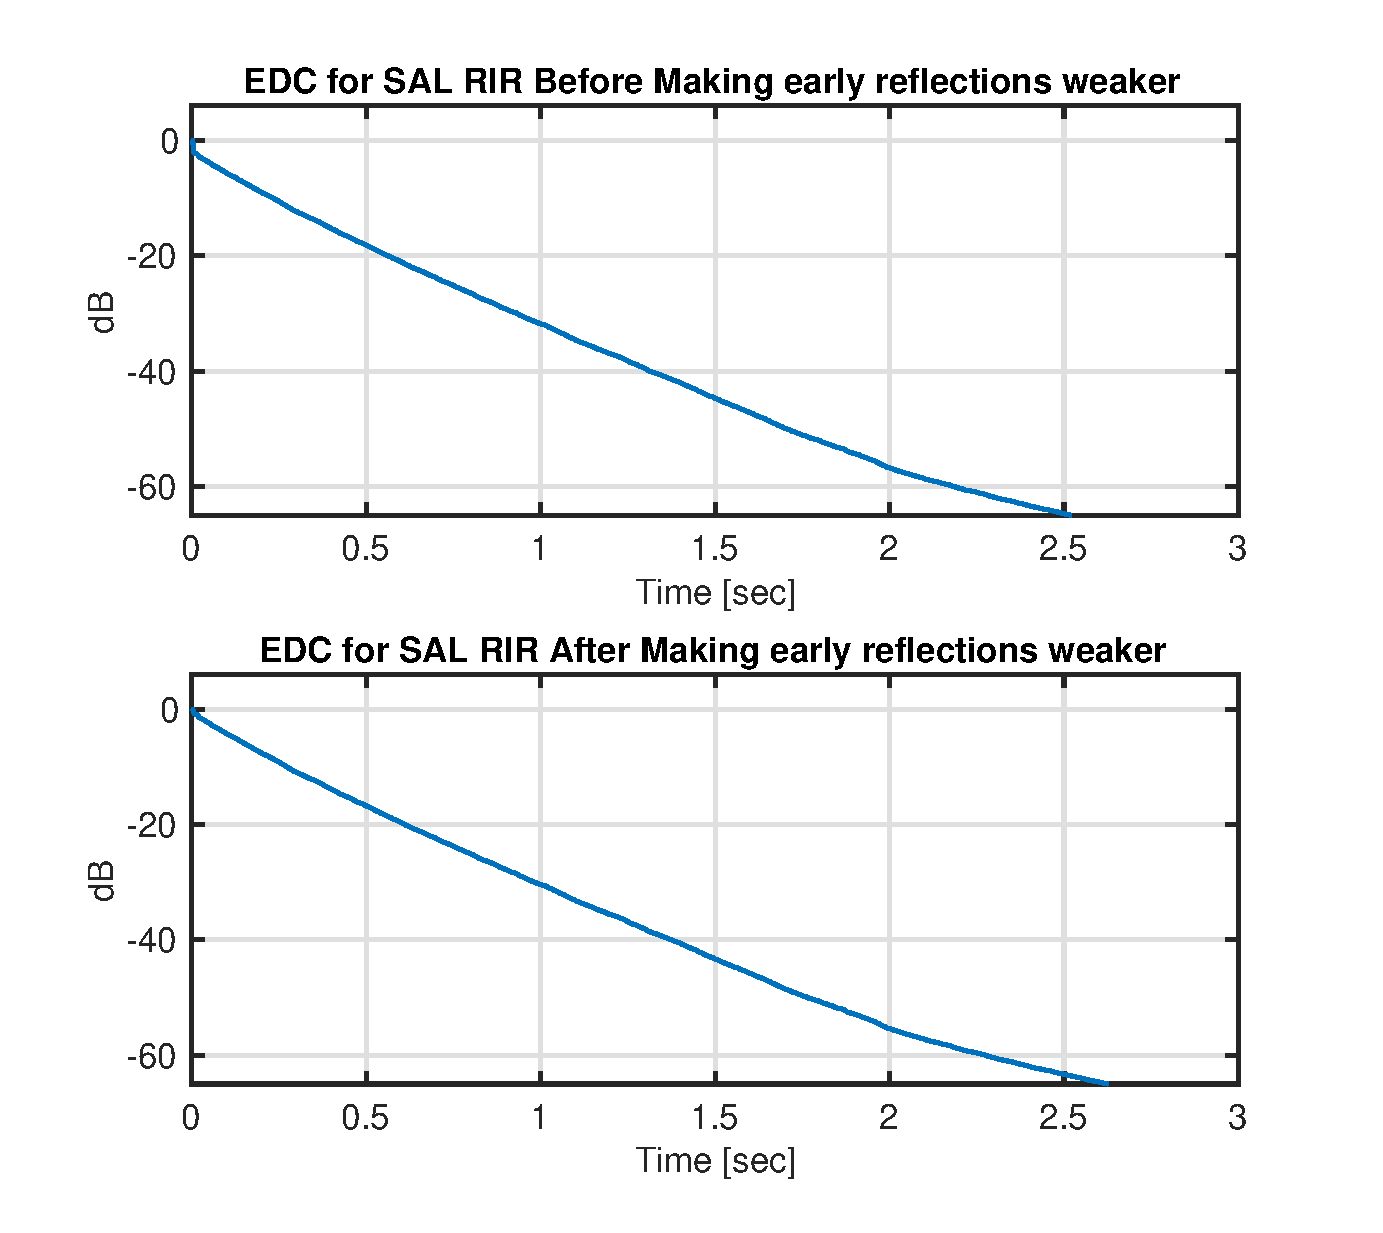
\includegraphics[width=\textwidth]{SAL_ERProcessingExample_Div2_EDC}
	\end{subfigure}
	\caption{Example of how early reflections of SAL RIR were reduced in magnitude (by 6 dB) to make reverberation effect stronger}
	\label{fig:SAL_ERProcessing_Div2}
\end{figure}

\begin{figure}[H]
	\centering
	\begin{subfigure}[b]{0.98\textwidth}
		\centering
		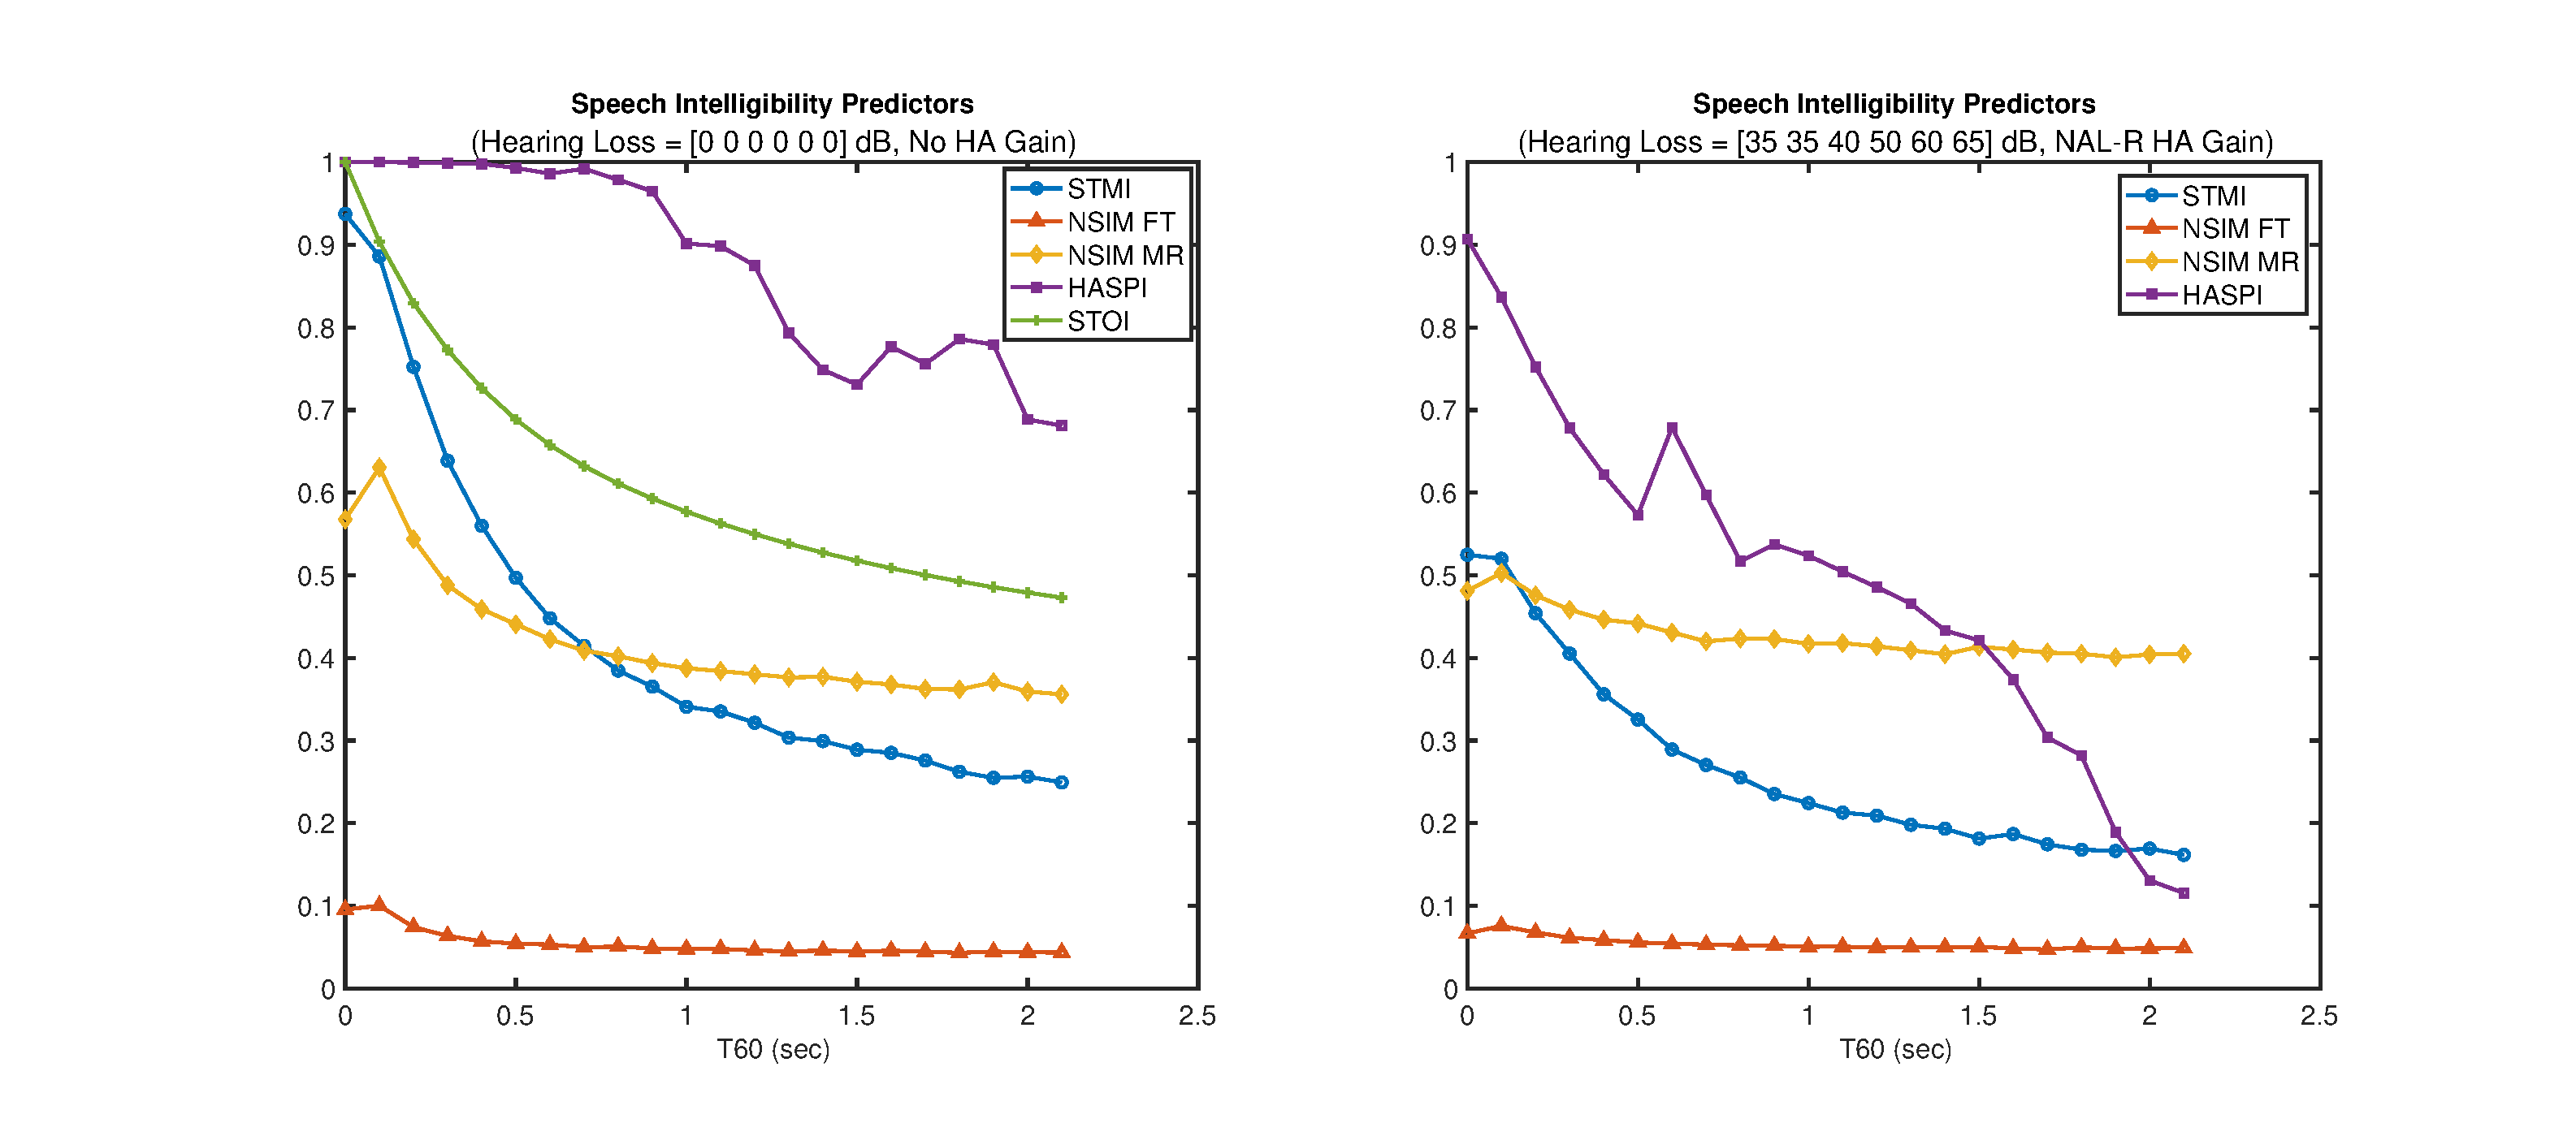
\includegraphics[width=\textwidth]{SAL_ERProcessingExample_Div2_SI}
	\end{subfigure}
	\caption{Impact of reducing early reflections of SAL RIR (i.e., Figure \ref{fig:SAL_ERProcessing_Div2}). SI shown before RIR processing (left) and after RIR processing (right) for comparison}
\label{fig:SAL_ERProcessing_Div2_SI_Results}
\end{figure}


- Discussion of how T60 is not a complete picture of the effects of reverb, EDT and SI together provide a more complete description. Generally speaking these are both encapsulated collectively in DRR

- Discussion of how NSIM and STMI continue to increase where HASPI plateaus suggesting that they can be used to reflect listening effort (NSIM and STMI still have some saturation, but not as much as subjective speech intelligibility). NSIM, STMI have no explicit application of a nonlinear  P/I function to map to SI, see notes about on how P/I function varies greatly depending on many factors so cant really be universal. The exact value of NSIM and STMI is not as meaningful, its moreso the how it changes with respect to control variables

- HASPI is mapped to SI, but I dont think it has an explicity P/I function -- not clear need to investigate. It clearly does strongly saturate in a way the resembles subjective SI more accurately

- Discussion of how NSIM and STMI were scaled (with a constant scaling factor accross all plots) to better view the trends accross all metrics on the same plot.

\begin{figure}[H]
	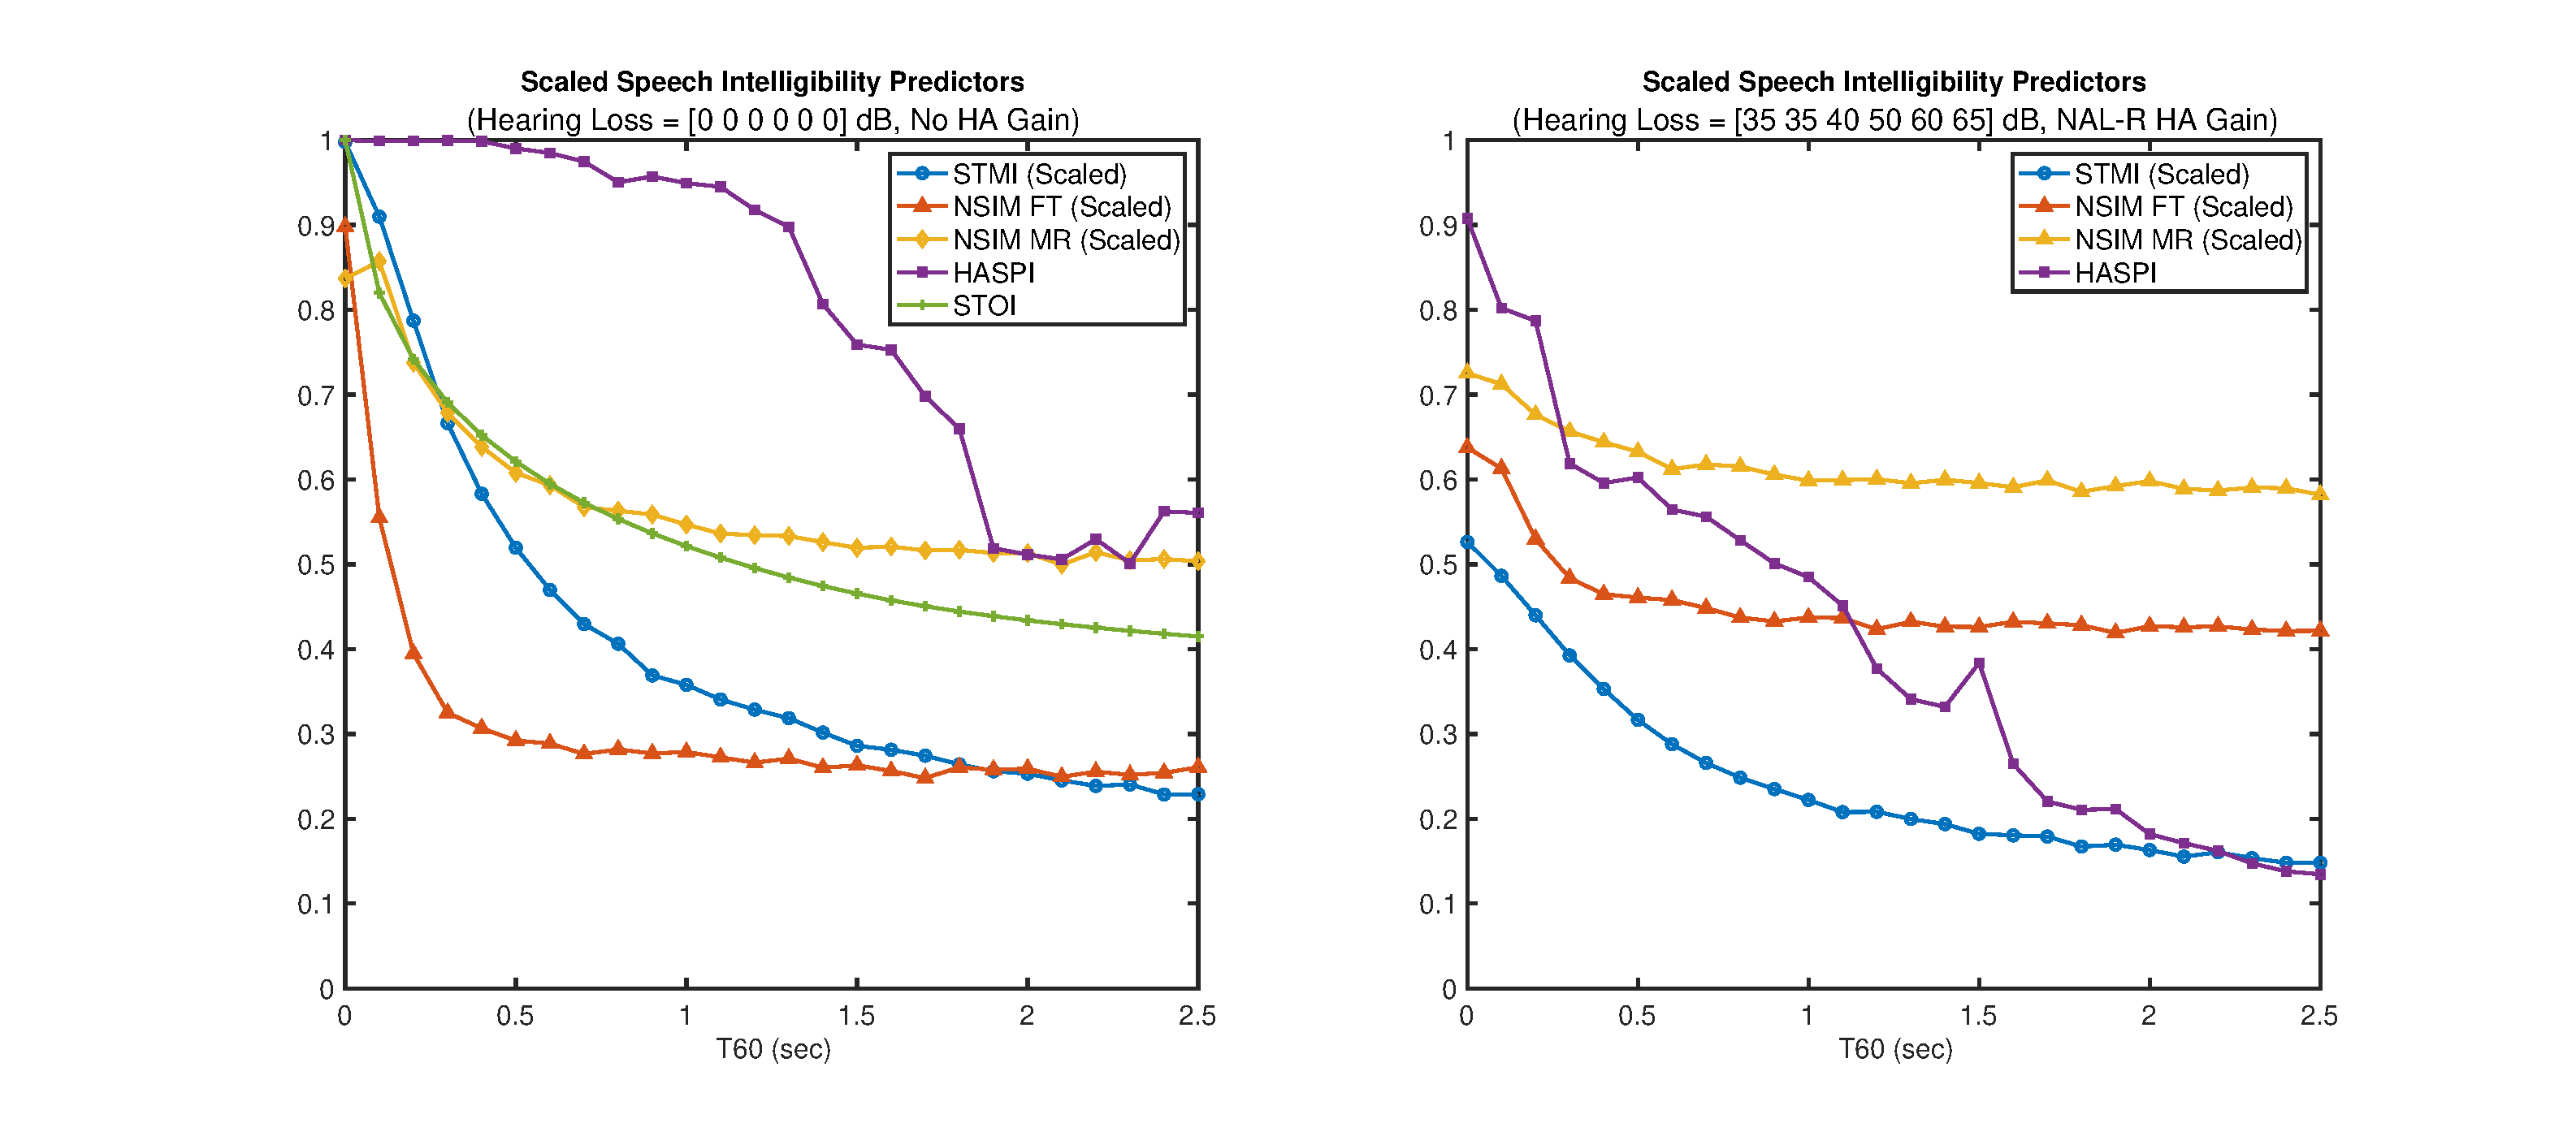
\includegraphics[width=0.98\textwidth]{SIMetricsEval_Synthetic_wScaling}
	\centering
	\caption{Impact of synthetic reverberation (exponentially decaying gaussian RIRs) on SI predictors with and without hearing loss. NAL-R linear hearing aid amplification included in hearing loss case for metrics that including modeling of hearing loss. Scaling applied to NSIM and STMI values to better view all metrics on the same plot.}
	\label{fig:SIMetricsEval_Synthetic_wScaling}
\end{figure}

\begin{figure}[H]
	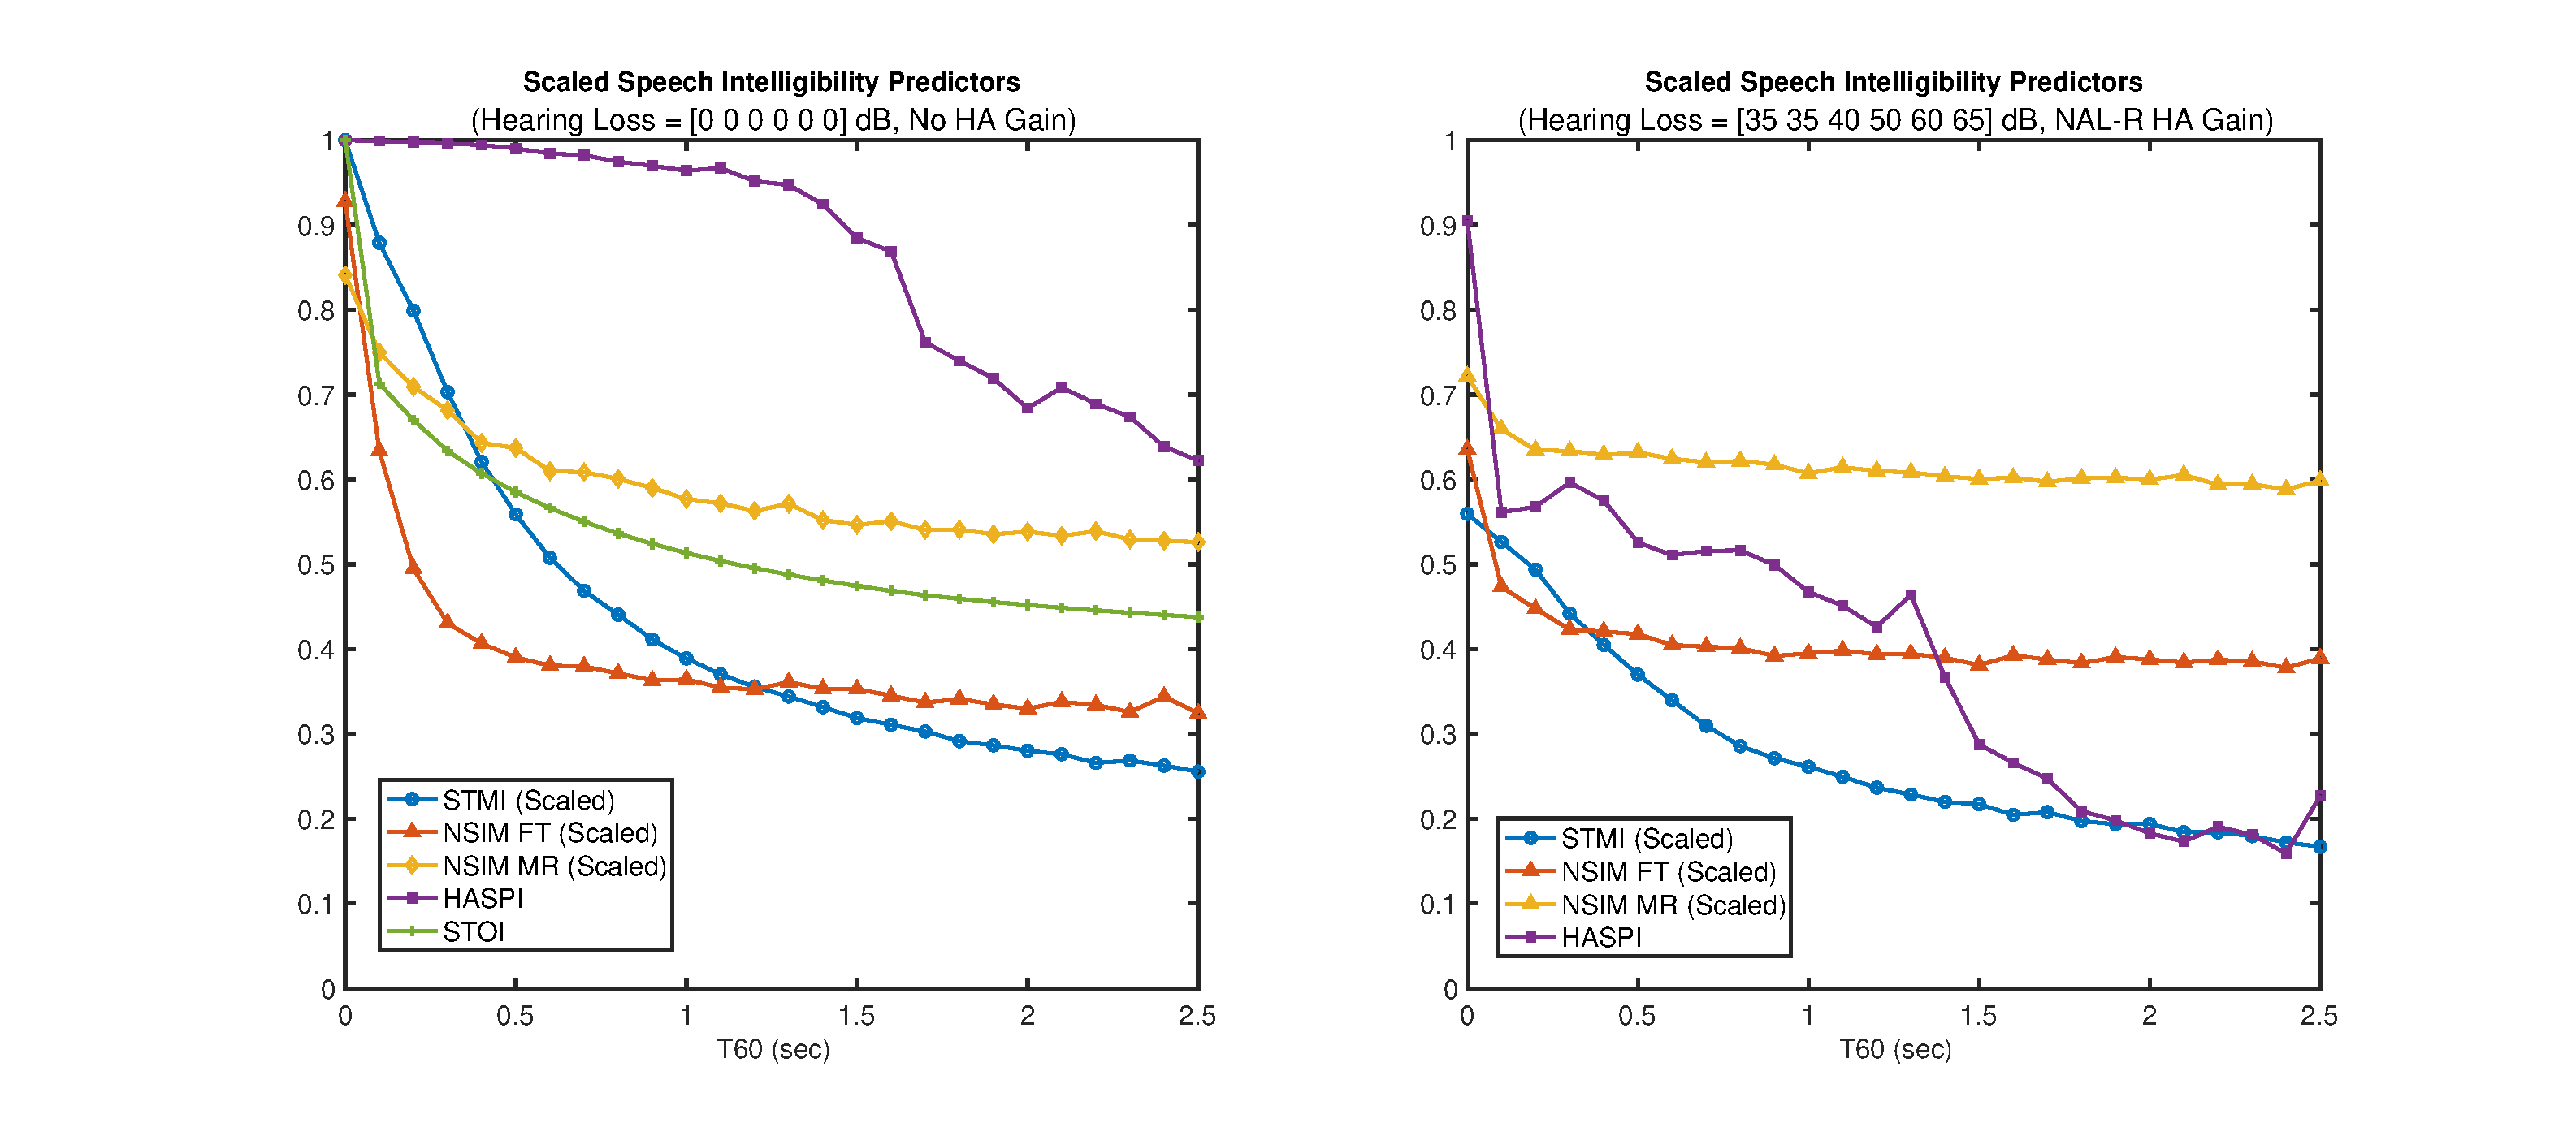
\includegraphics[width=0.98\textwidth]{SIMetricsEval_Synthetic_RealER_wScaling}
	\centering
	\caption{Impact of synthetic reverberation (exponentially decaying gaussian RIRs) with added real early reflections generated by truncating a real RIR  (Office II RIR from the HRIR database) on SI predictors with and without hearing loss. NAL-R linear hearing aid amplification included in hearing loss case for metrics that including modeling of hearing loss. Scaling applied to NSIM and STMI values to better view all metrics on the same plot.}
	\label{fig:SIMetricsEval_Synthetic_RealER_wScaling}
\end{figure}

\begin{figure}[H]
	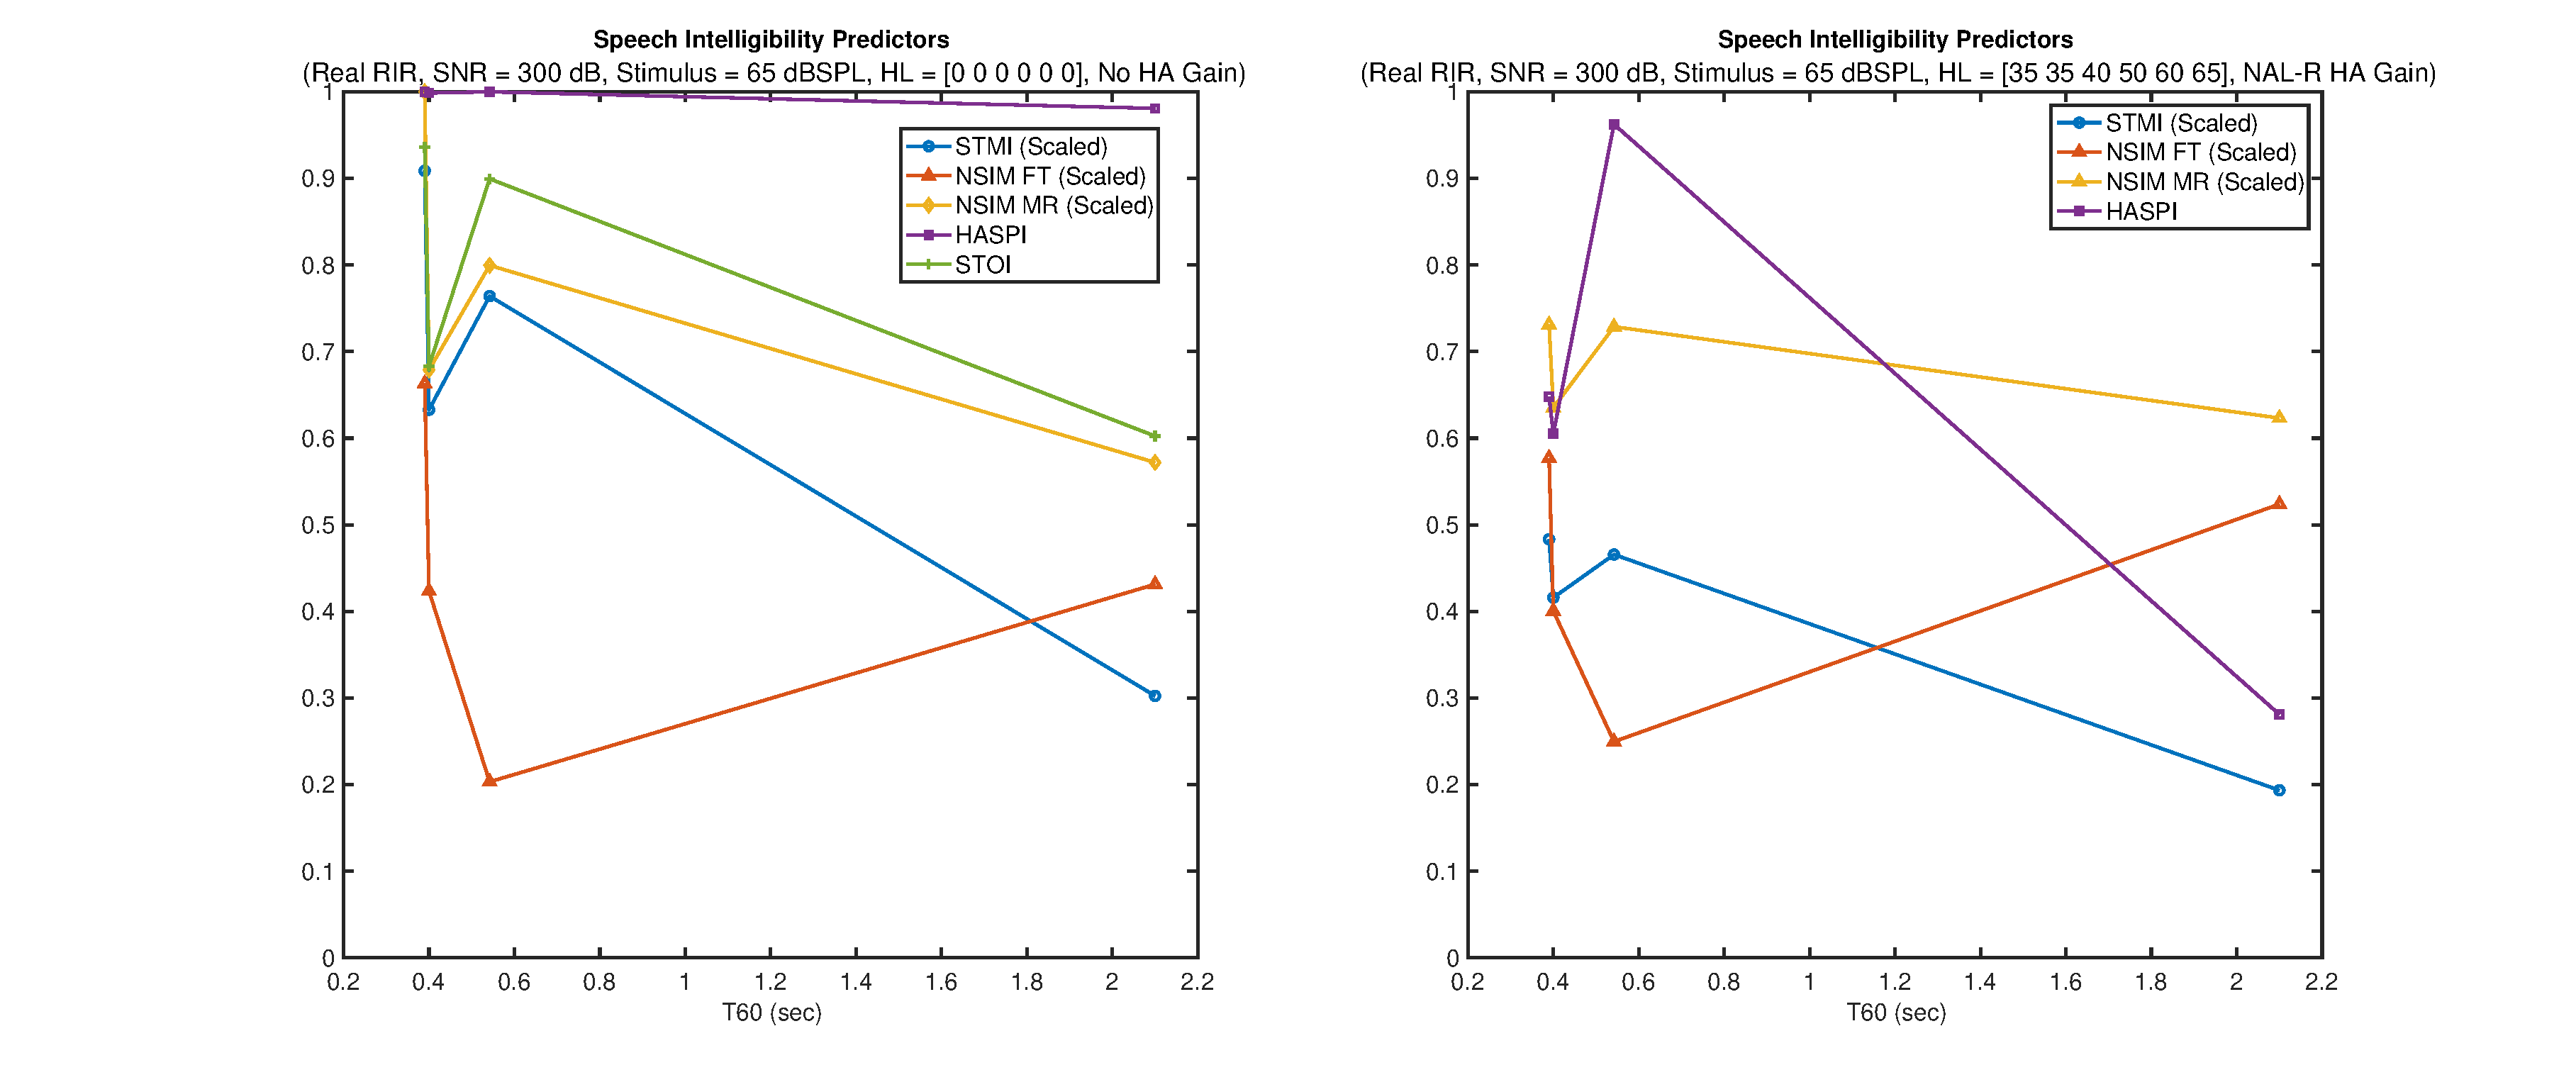
\includegraphics[width=0.98\textwidth]{SIMetricsEval_Real_wScaling}
	\centering
	\caption{Impact of practical reverberation (several real measured RIRs) on SI predictors with and without hearing loss. NAL-R linear hearing aid amplification included in hearing loss case for metrics that including modeling of hearing loss.  Scaling applied to NSIM and STMI values to better view all metrics on the same plot.}
	\label{fig:SIMetricsEval_Real_wScaling}
\end{figure}

\begin{figure}[H]
	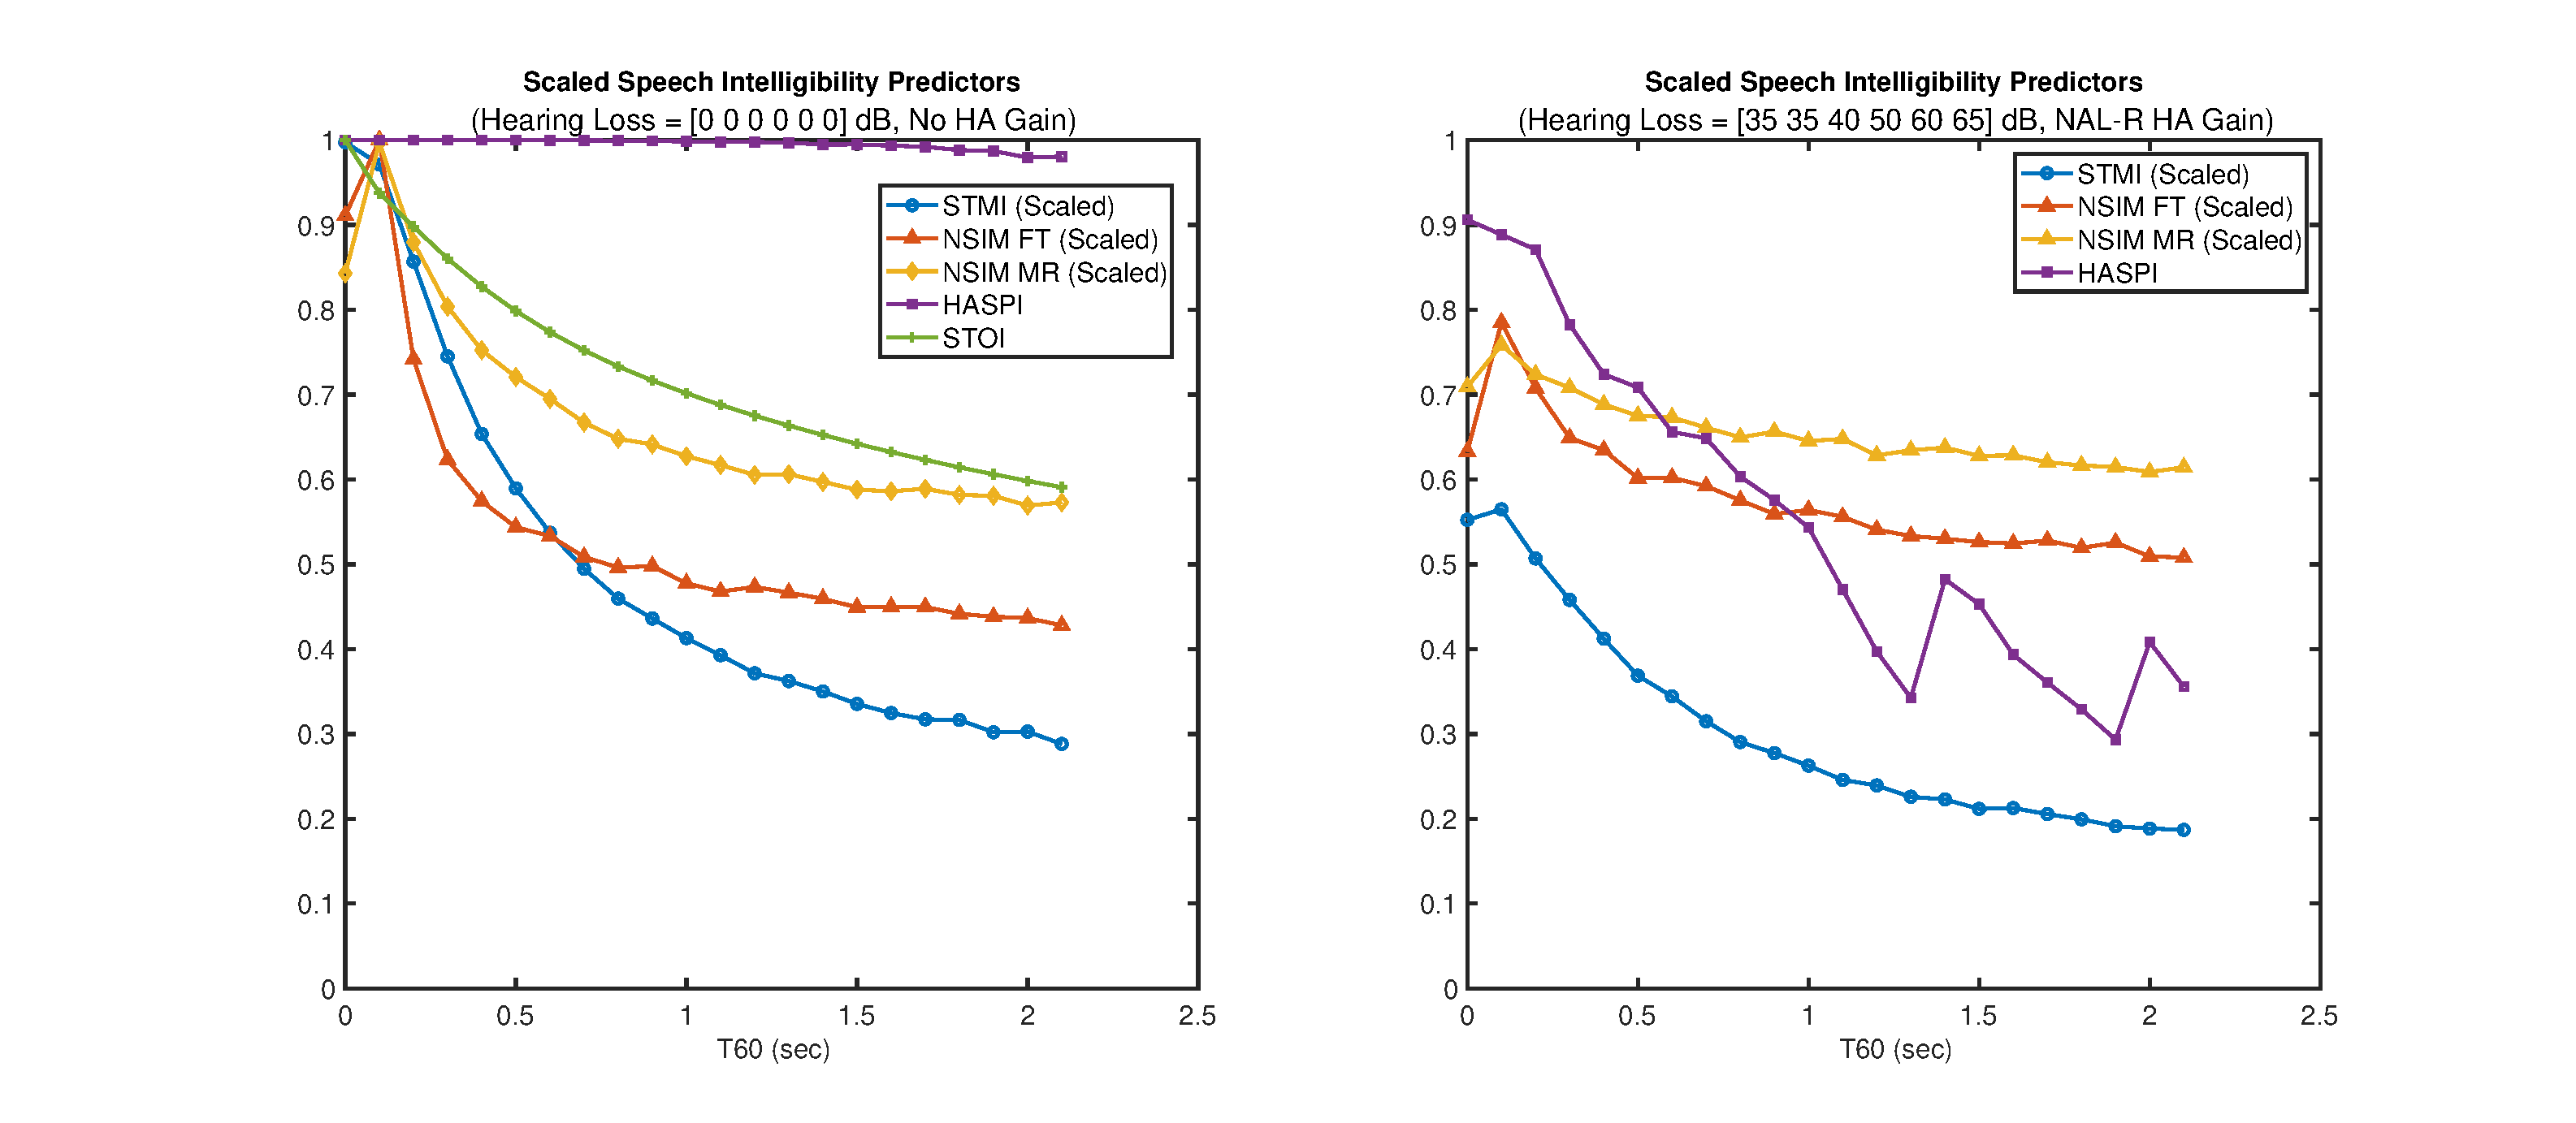
\includegraphics[width=0.98\textwidth]{SIMetricsEval_TruncatedSAL_wScaling}
	\centering
	\caption{Impact of practical reverberation (SAL room from MYRiAD database exponentially truncated to control T60) on SI predictors with and without hearing loss. NAL-R linear hearing aid amplification included in hearing loss case for metrics that including modeling of hearing loss.  Scaling applied to NSIM and STMI values to better view all metrics on the same plot.}
	\label{fig:SIMetricsEval_TruncatedSAL_wScaling}
\end{figure}

\section{Final Method Used}

%\begin{sidewaysfigure}[H]
%	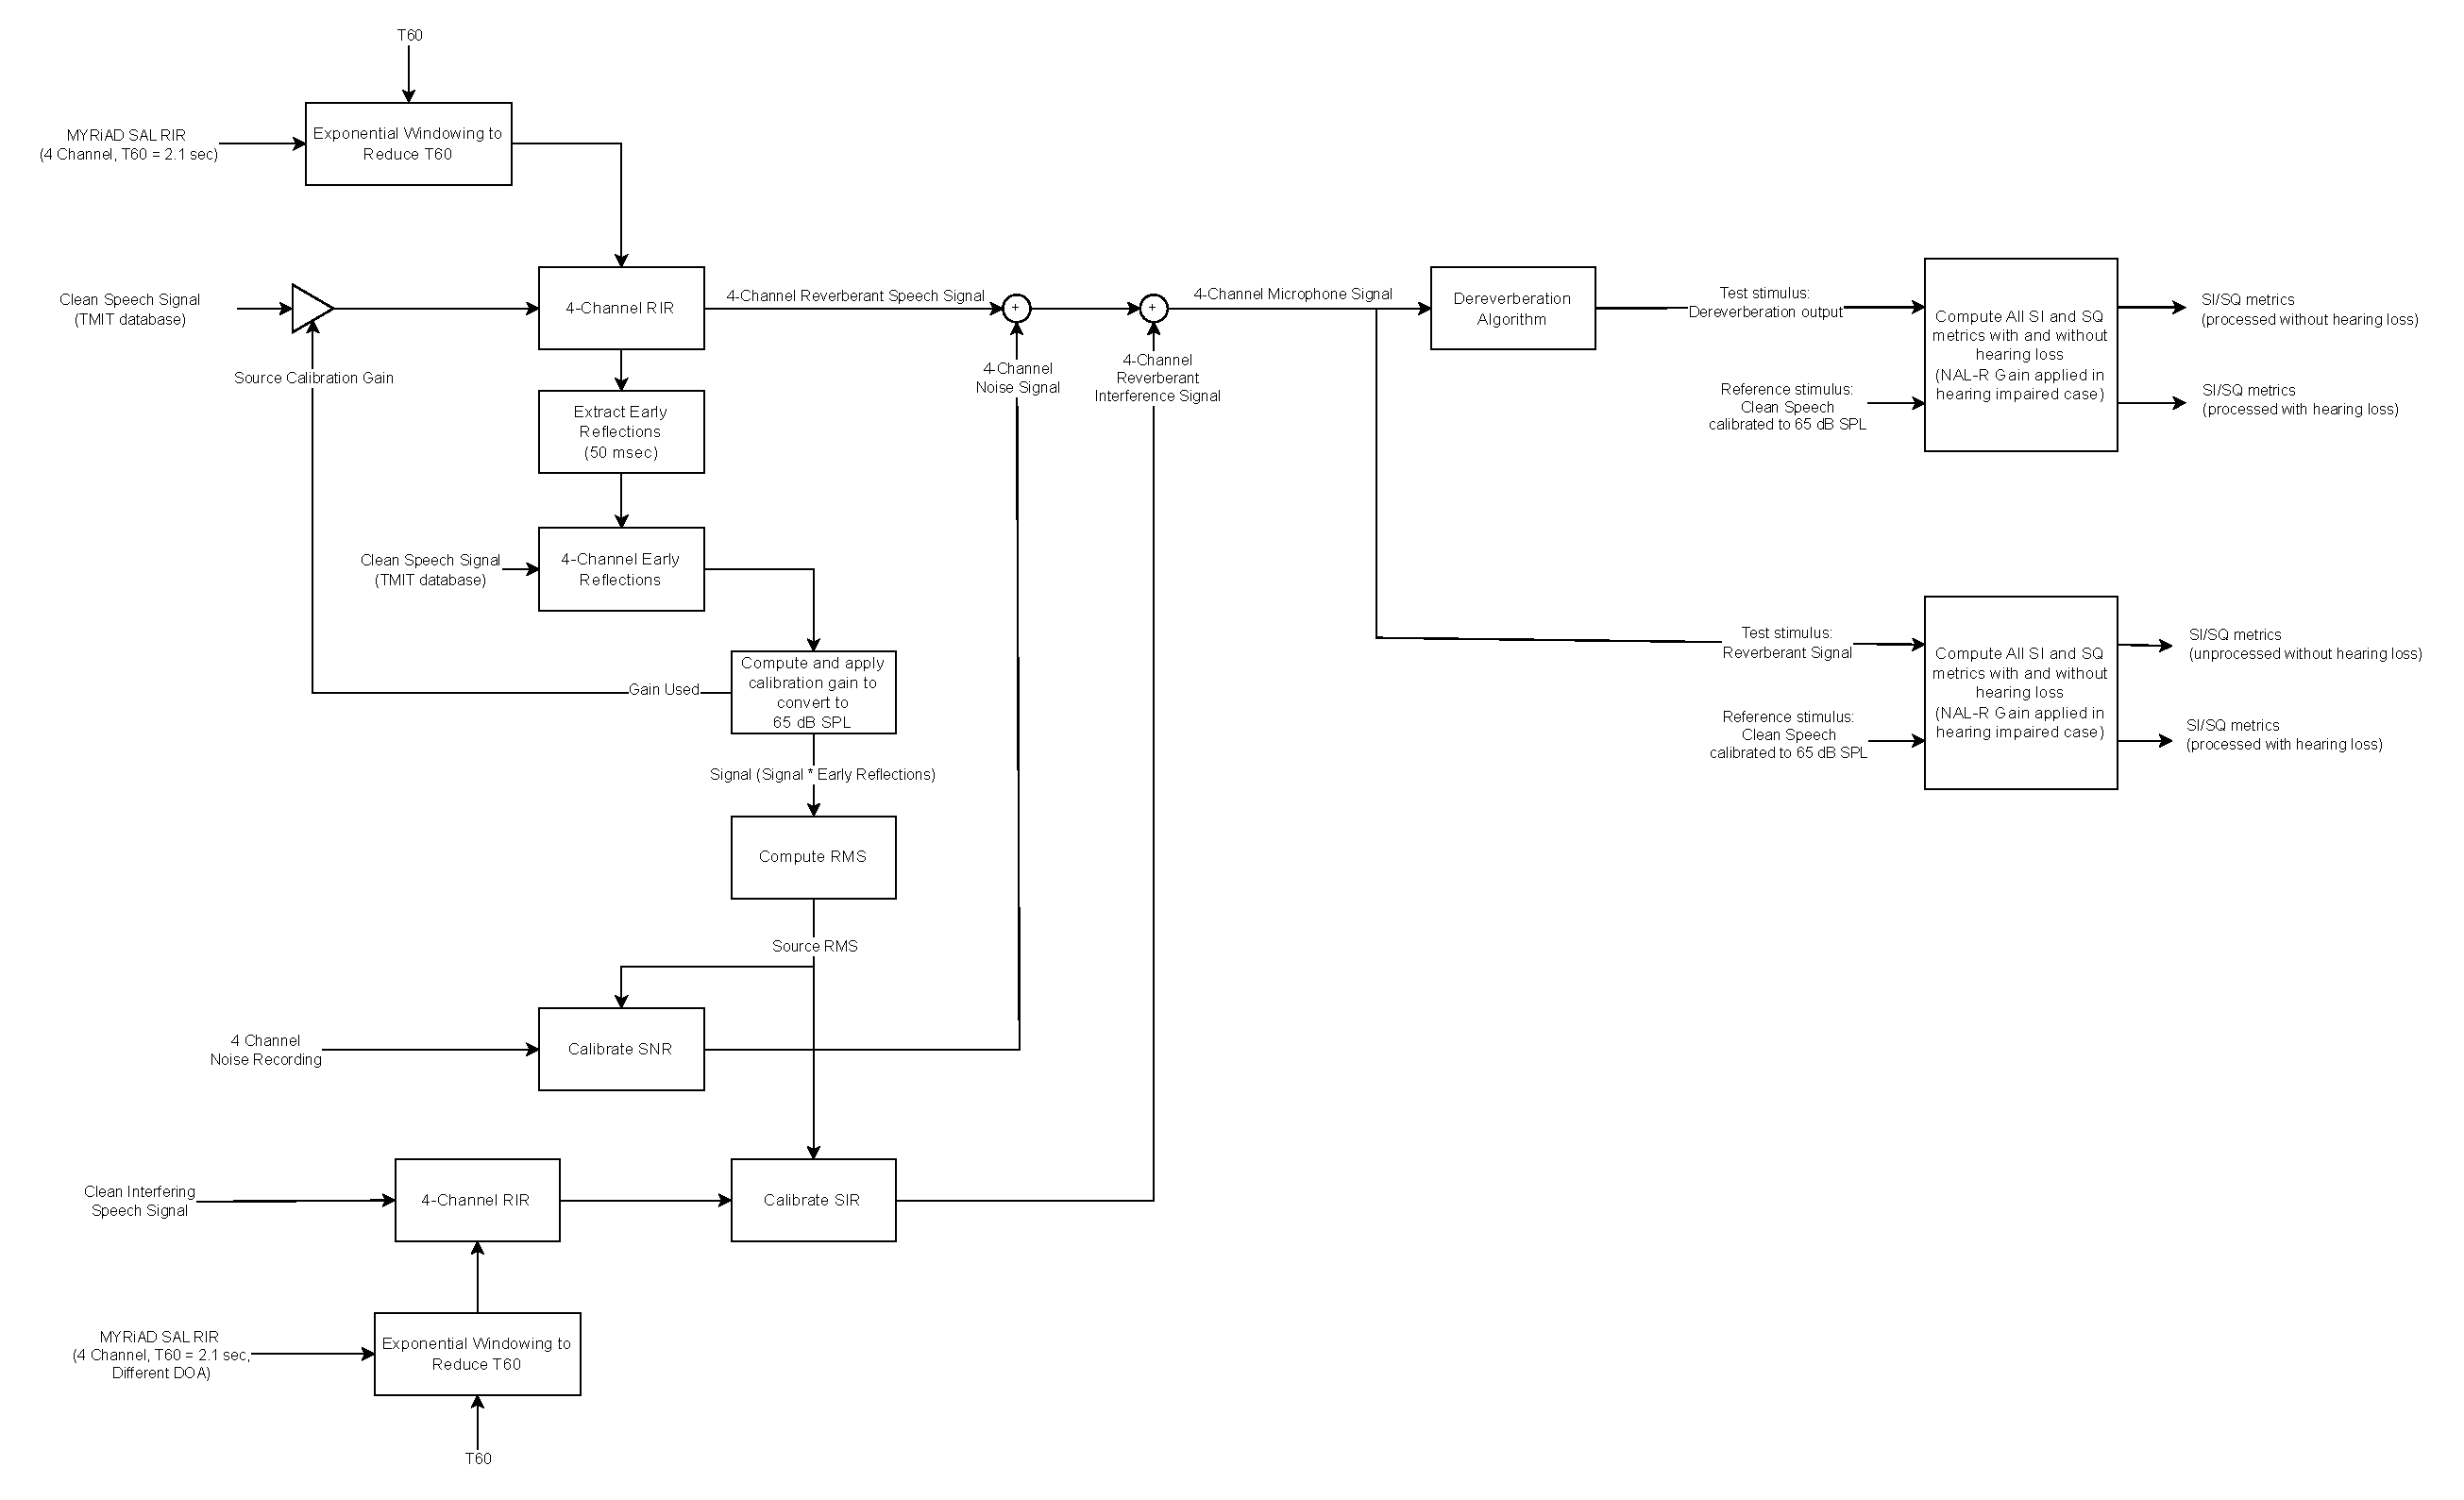
\includegraphics[height=0.9\textheight]{ThesisExperimentMethod}
%	\centering
%	\caption{Block diagram for method used in evaluating dereverberation algorithm performance. Microphone signals include reverberant speech (MYRiAD SAL RIR windowed exponentially to control T60) with added noise signal (real multichannel noise recordings) and added reverberant interference signal. All SI and SQ predictors were computed for the unprocessed microphone signals and the dereverberation output both with and without hearing loss included in all models of speech perception.}
%	\label{fig:Evaluation_Block_Diagram}
%\end{sidewaysfigure}

\begin{sidewaysfigure}
	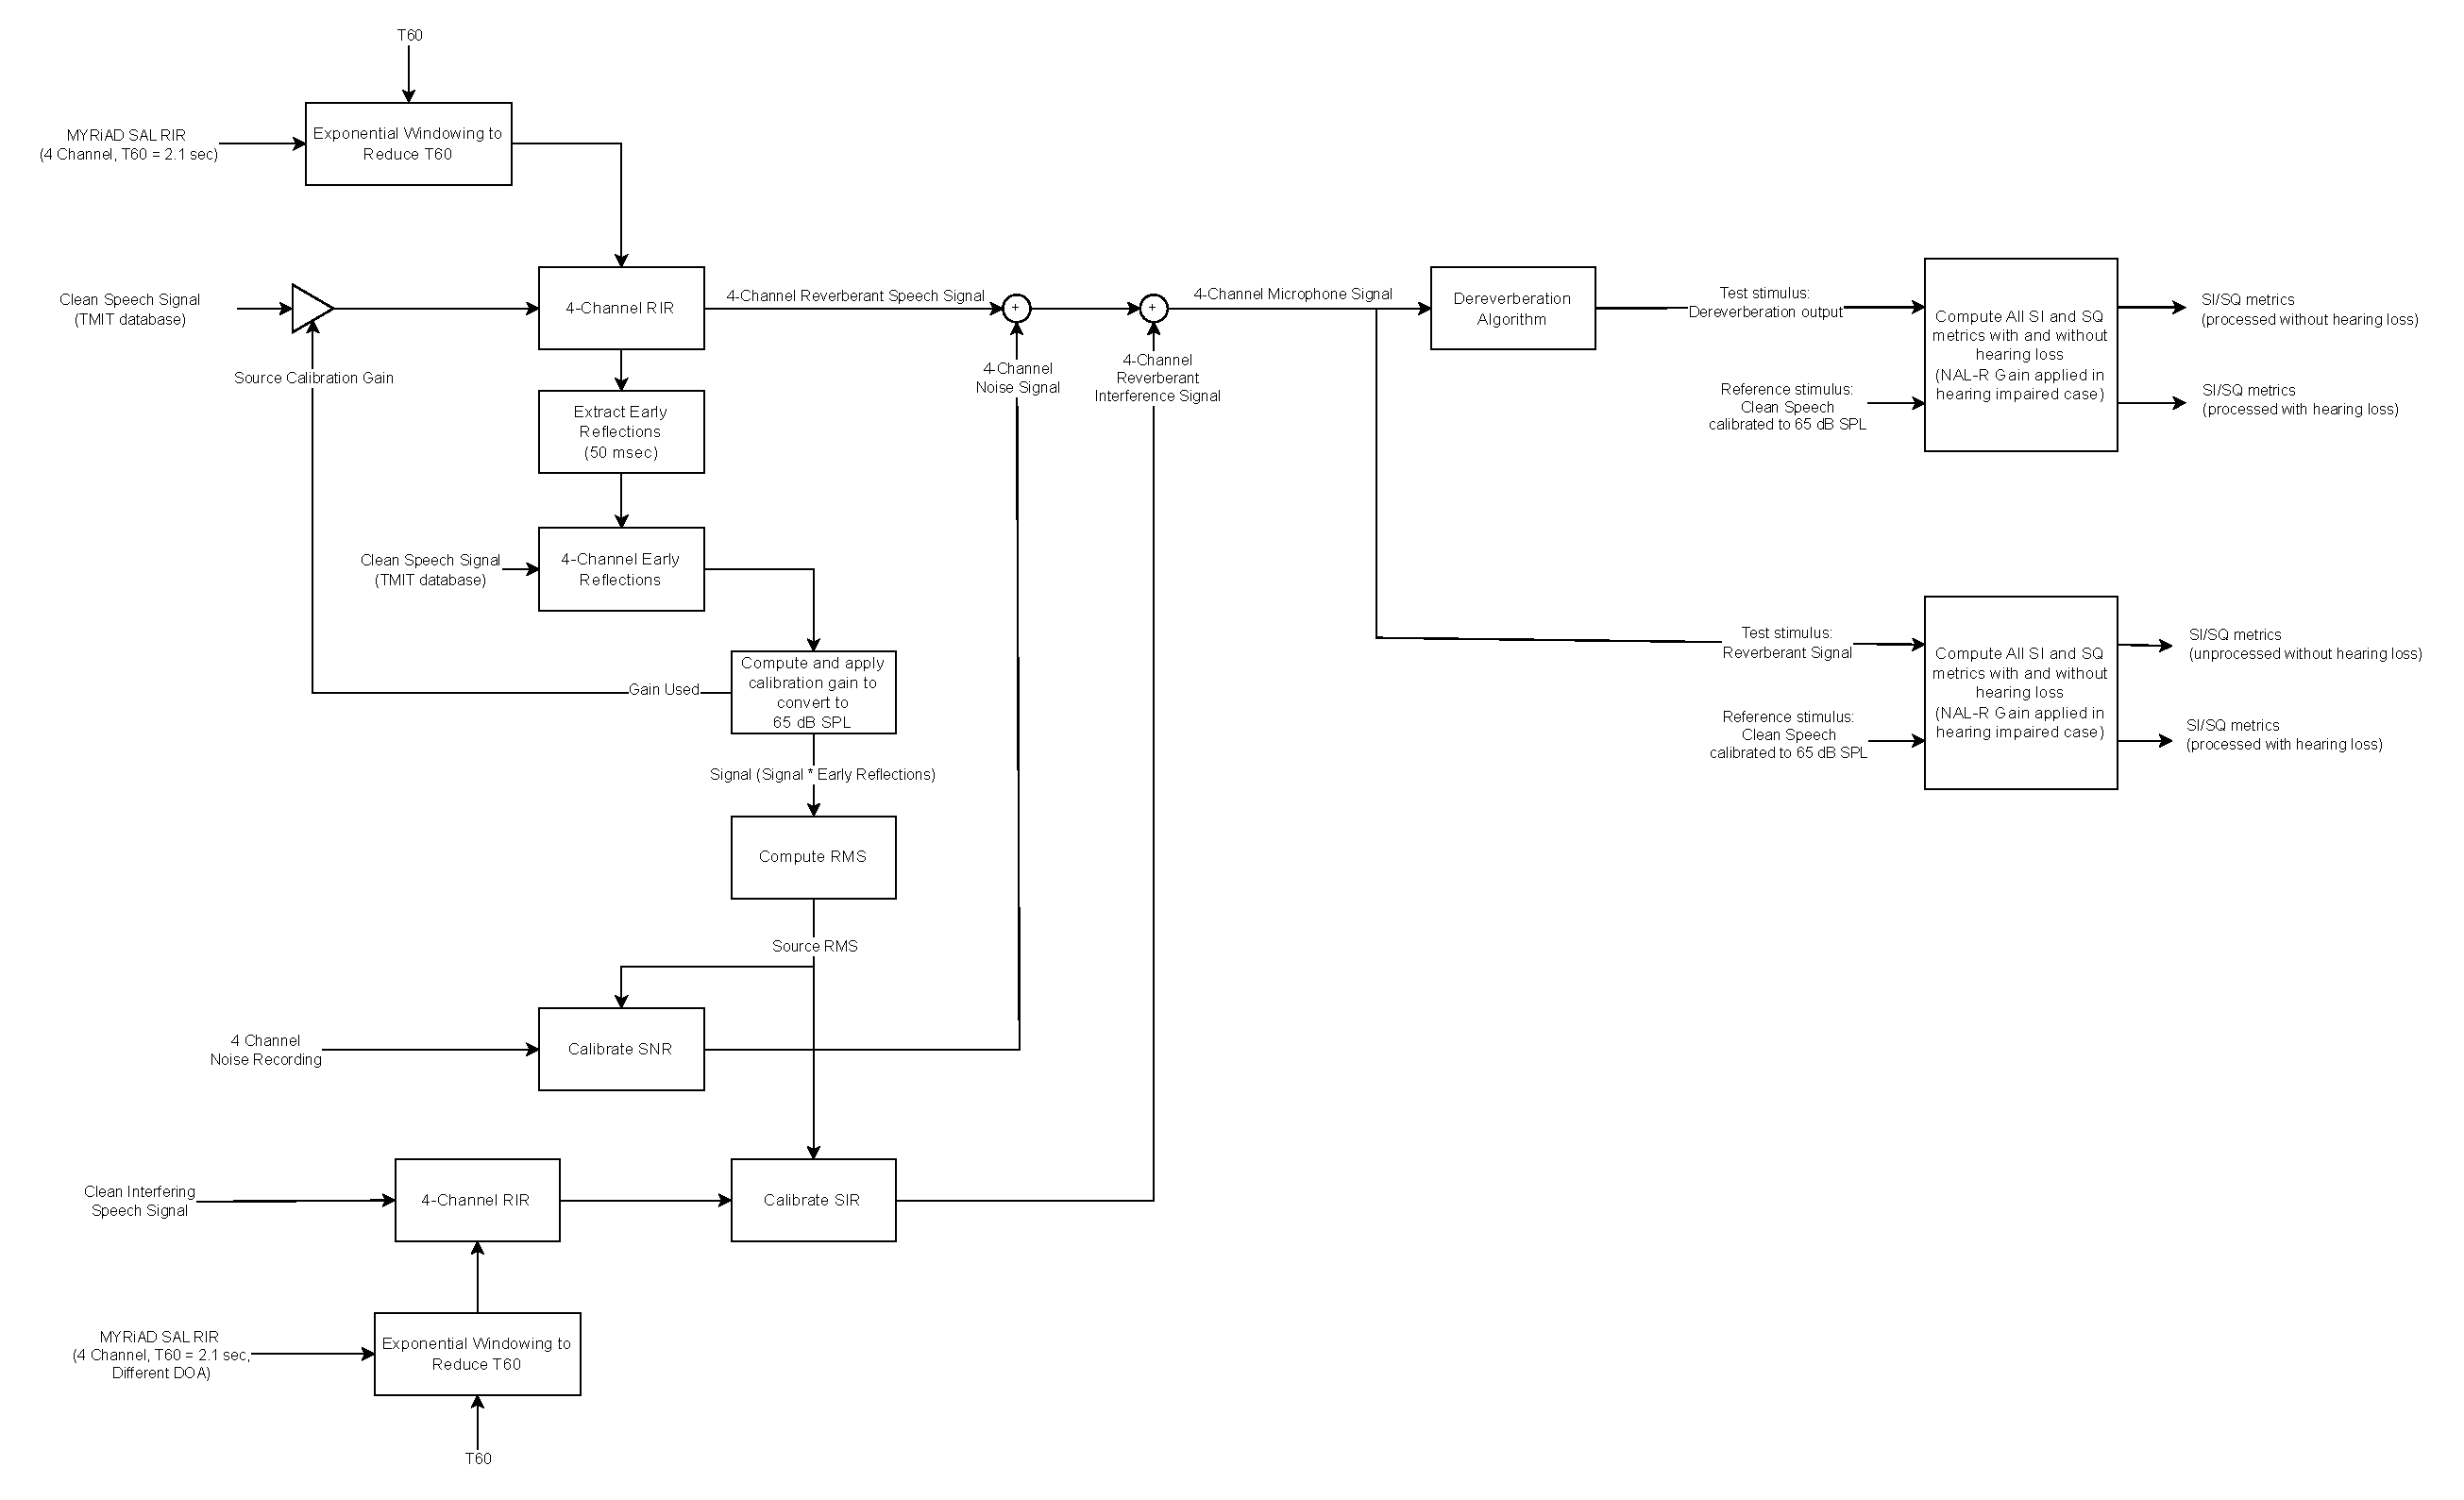
\includegraphics[width=\columnwidth]{ThesisExperimentMethod}%
	\label{fig:Evaluation_Block_Diagram}
	\caption{Block diagram for method used in evaluating dereverberation algorithm performance. Microphone signals include reverberant speech (MYRiAD SAL RIR windowed exponentially to control T60) with added noise signal (real multichannel noise recordings) and added reverberant interference signal. All SI and SQ predictors were computed for the unprocessed microphone signals and the dereverberation output both with and without hearing loss included in all models of speech perception.}
\end{sidewaysfigure}




\section{Delay-and-Predict Dereverberation Evaluation with Synthetic Reverberation}

\textbf{SI/SQ/Clarity v T60 w/ no noise}

\begin{figure}[H]
	\centering
	\begin{subfigure}[b]{0.47\textwidth}
		\centering
		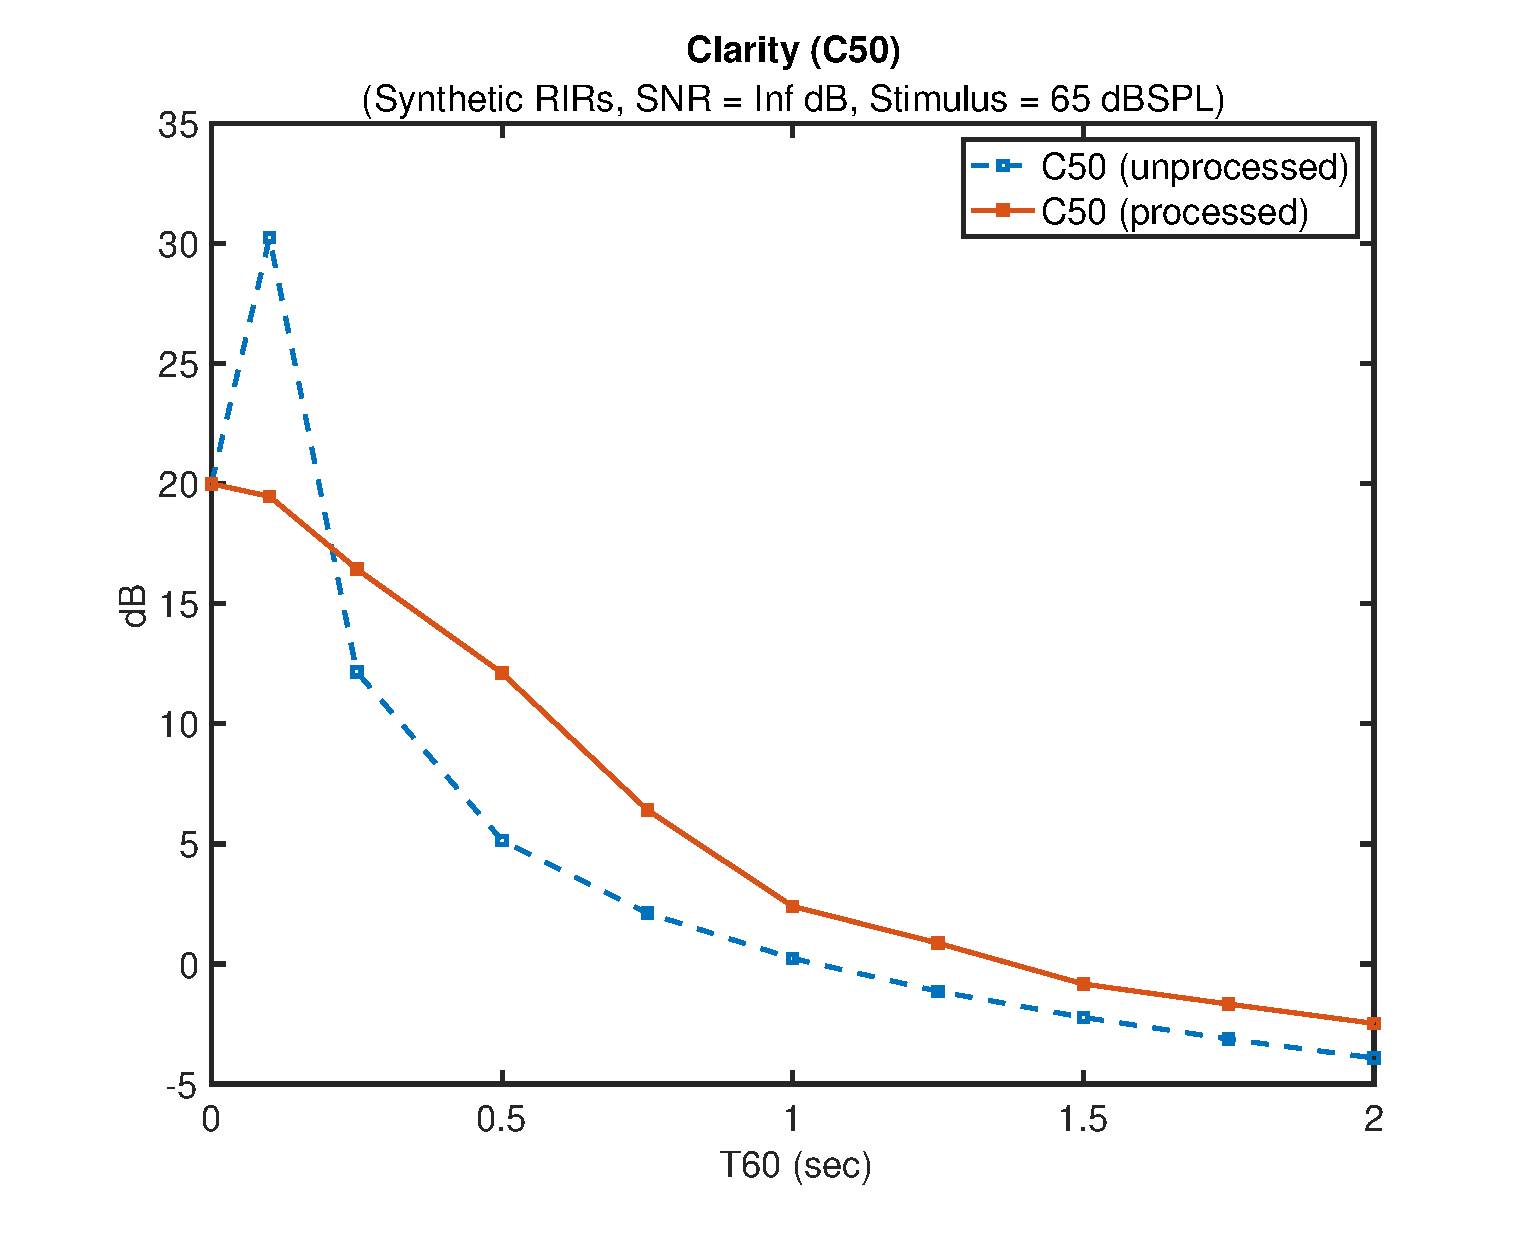
\includegraphics[width=\textwidth]{DAP_EvalT60Sweep_Synthetic_NoNoise_C50_v_T60}
	\end{subfigure}
	\begin{subfigure}[b]{0.92\textwidth}
		\centering
		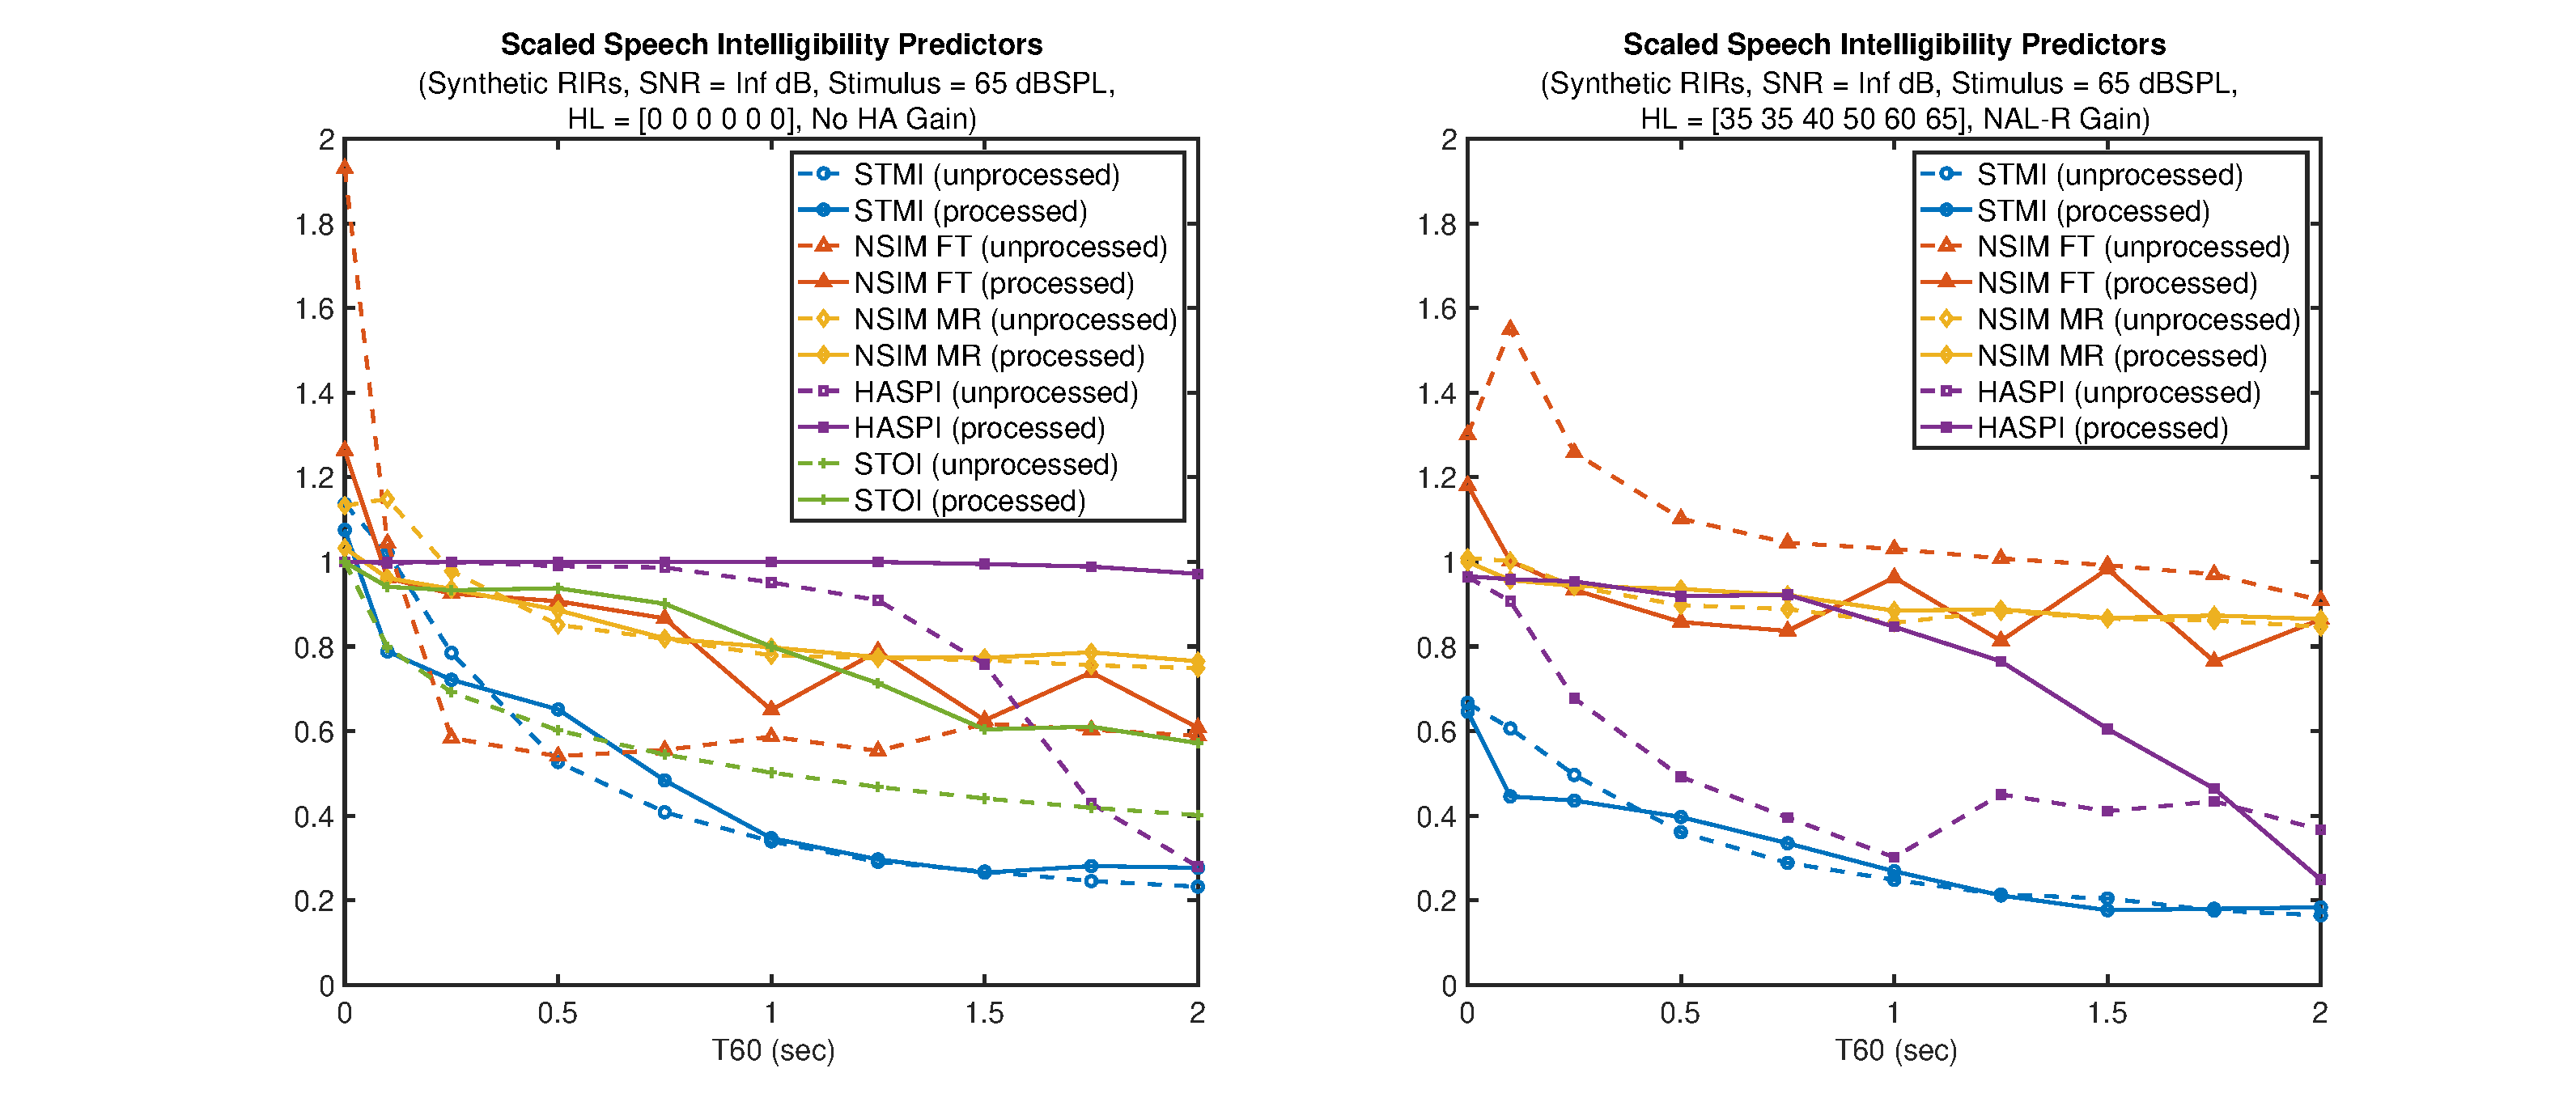
\includegraphics[width=\textwidth]{DAP_EvalT60Sweep_Synthetic_NoNoise_SI_v_T60}
	\end{subfigure}
	\begin{subfigure}[b]{0.92\textwidth}
		\centering
		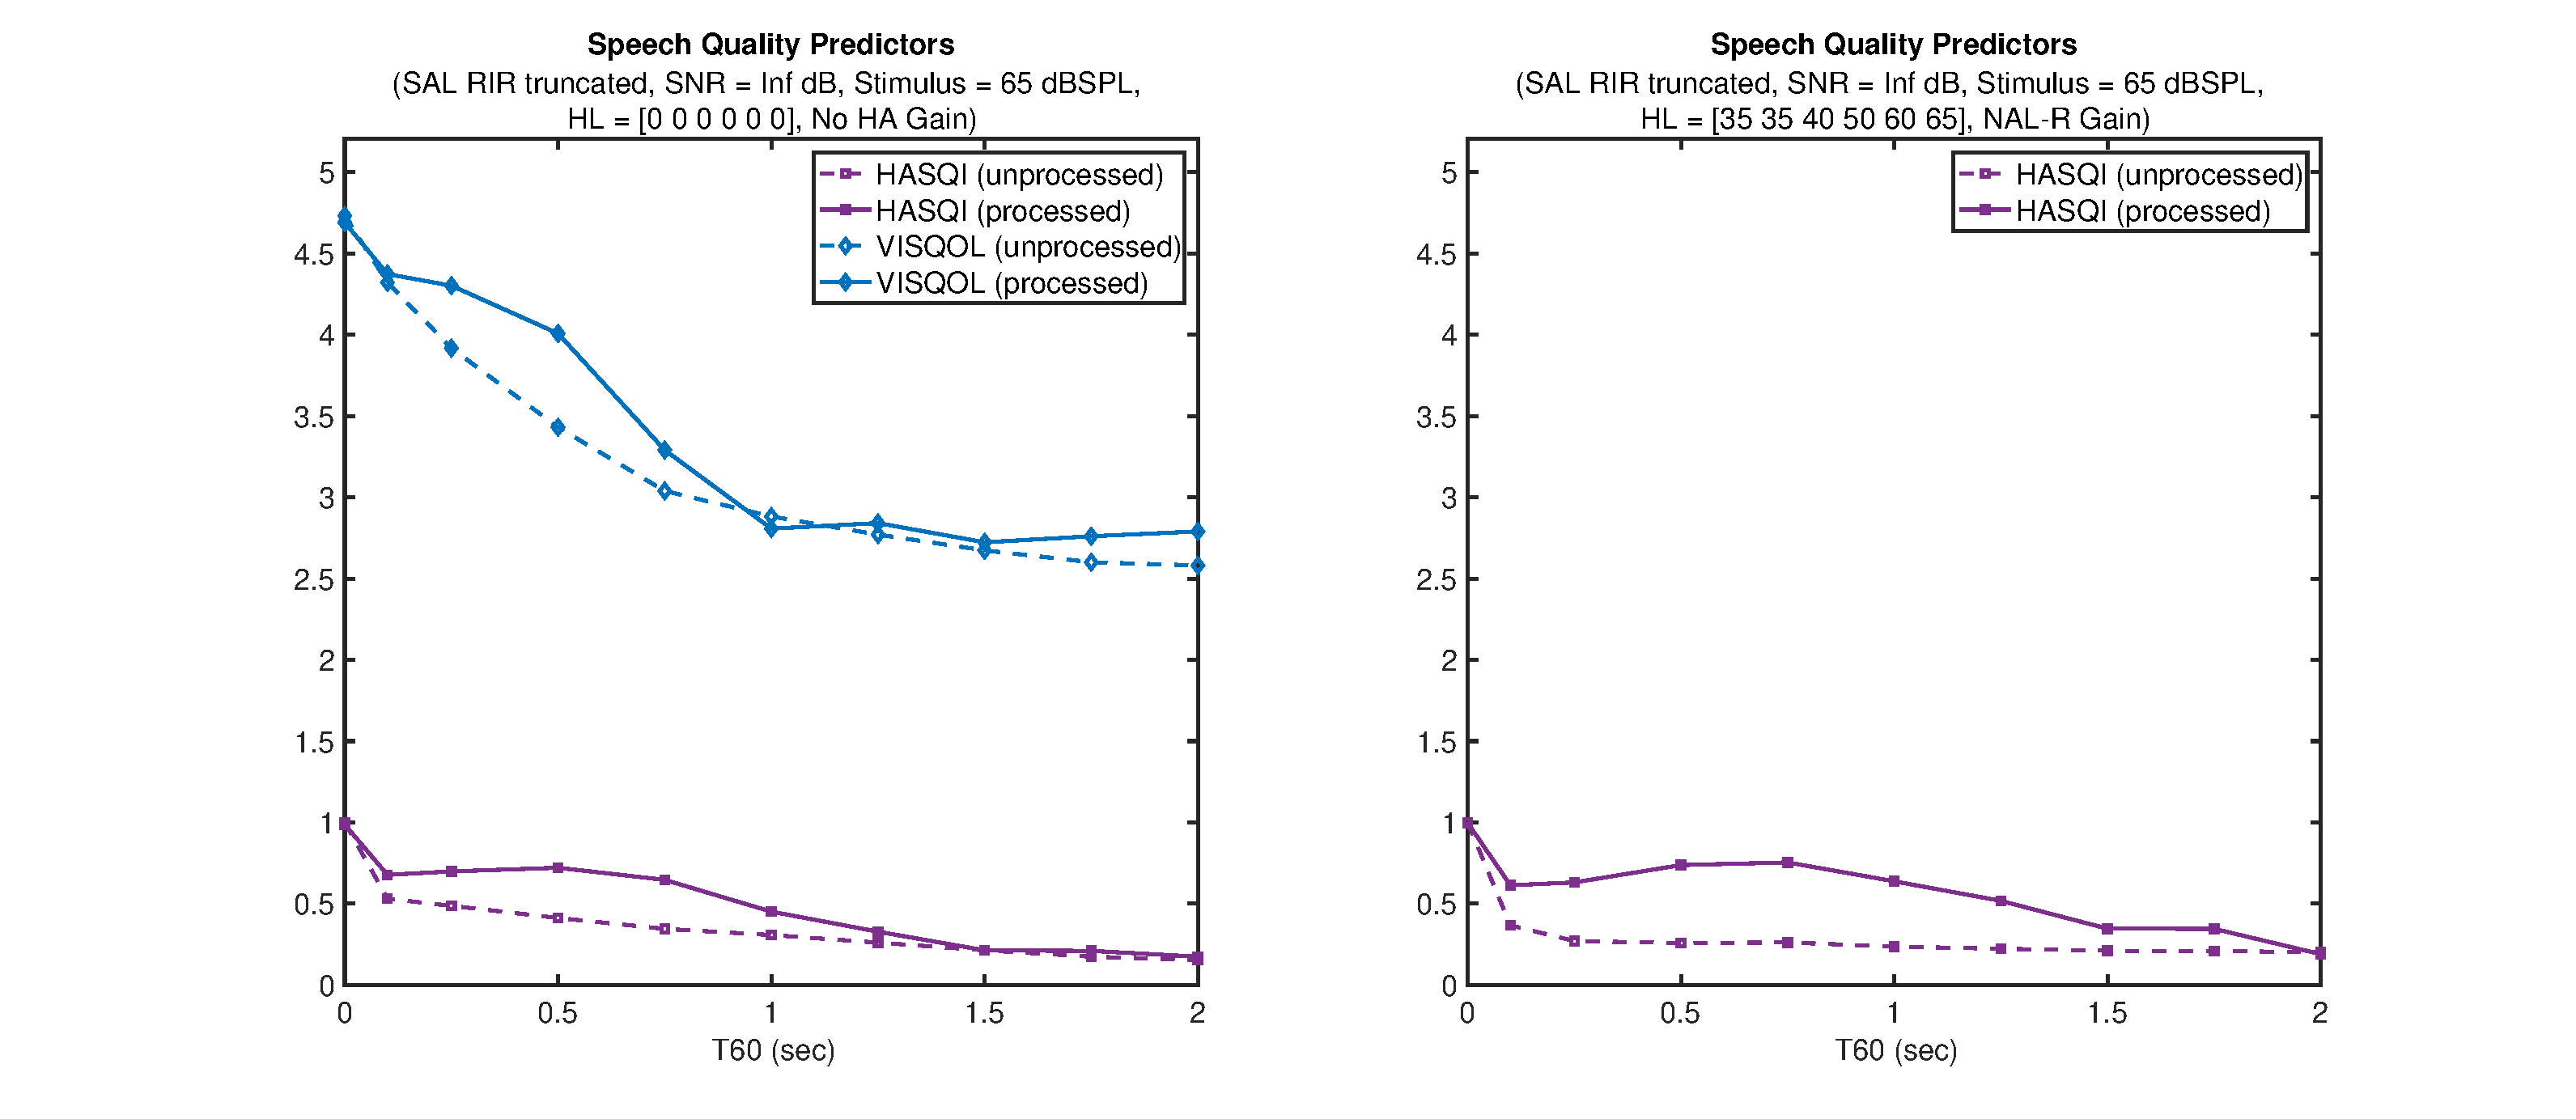
\includegraphics[width=\textwidth]{DAP_EvalT60Sweep_Synthetic_NoNoise_SQ_v_T60}
	\end{subfigure}
	\caption{Evaluation of delay-and-predict dereverberation performance as a function of T60. RIRs were synthetically generated by applying a variable decay-rate exponential window to sequences of uncorrelated Gaussian white noise.}
	\label{fig:DAP_EvalT60Sweep_Synthetic_NoNoise}
\end{figure}

\section{Delay-and-Predict Dereverberation Evaluation with Realistic Reverberation}

\textbf{SI/SQ/Clarity v T60 w/ no noise}

\begin{figure}[H]
	\centering
	\begin{subfigure}[b]{0.47\textwidth}
		\centering
		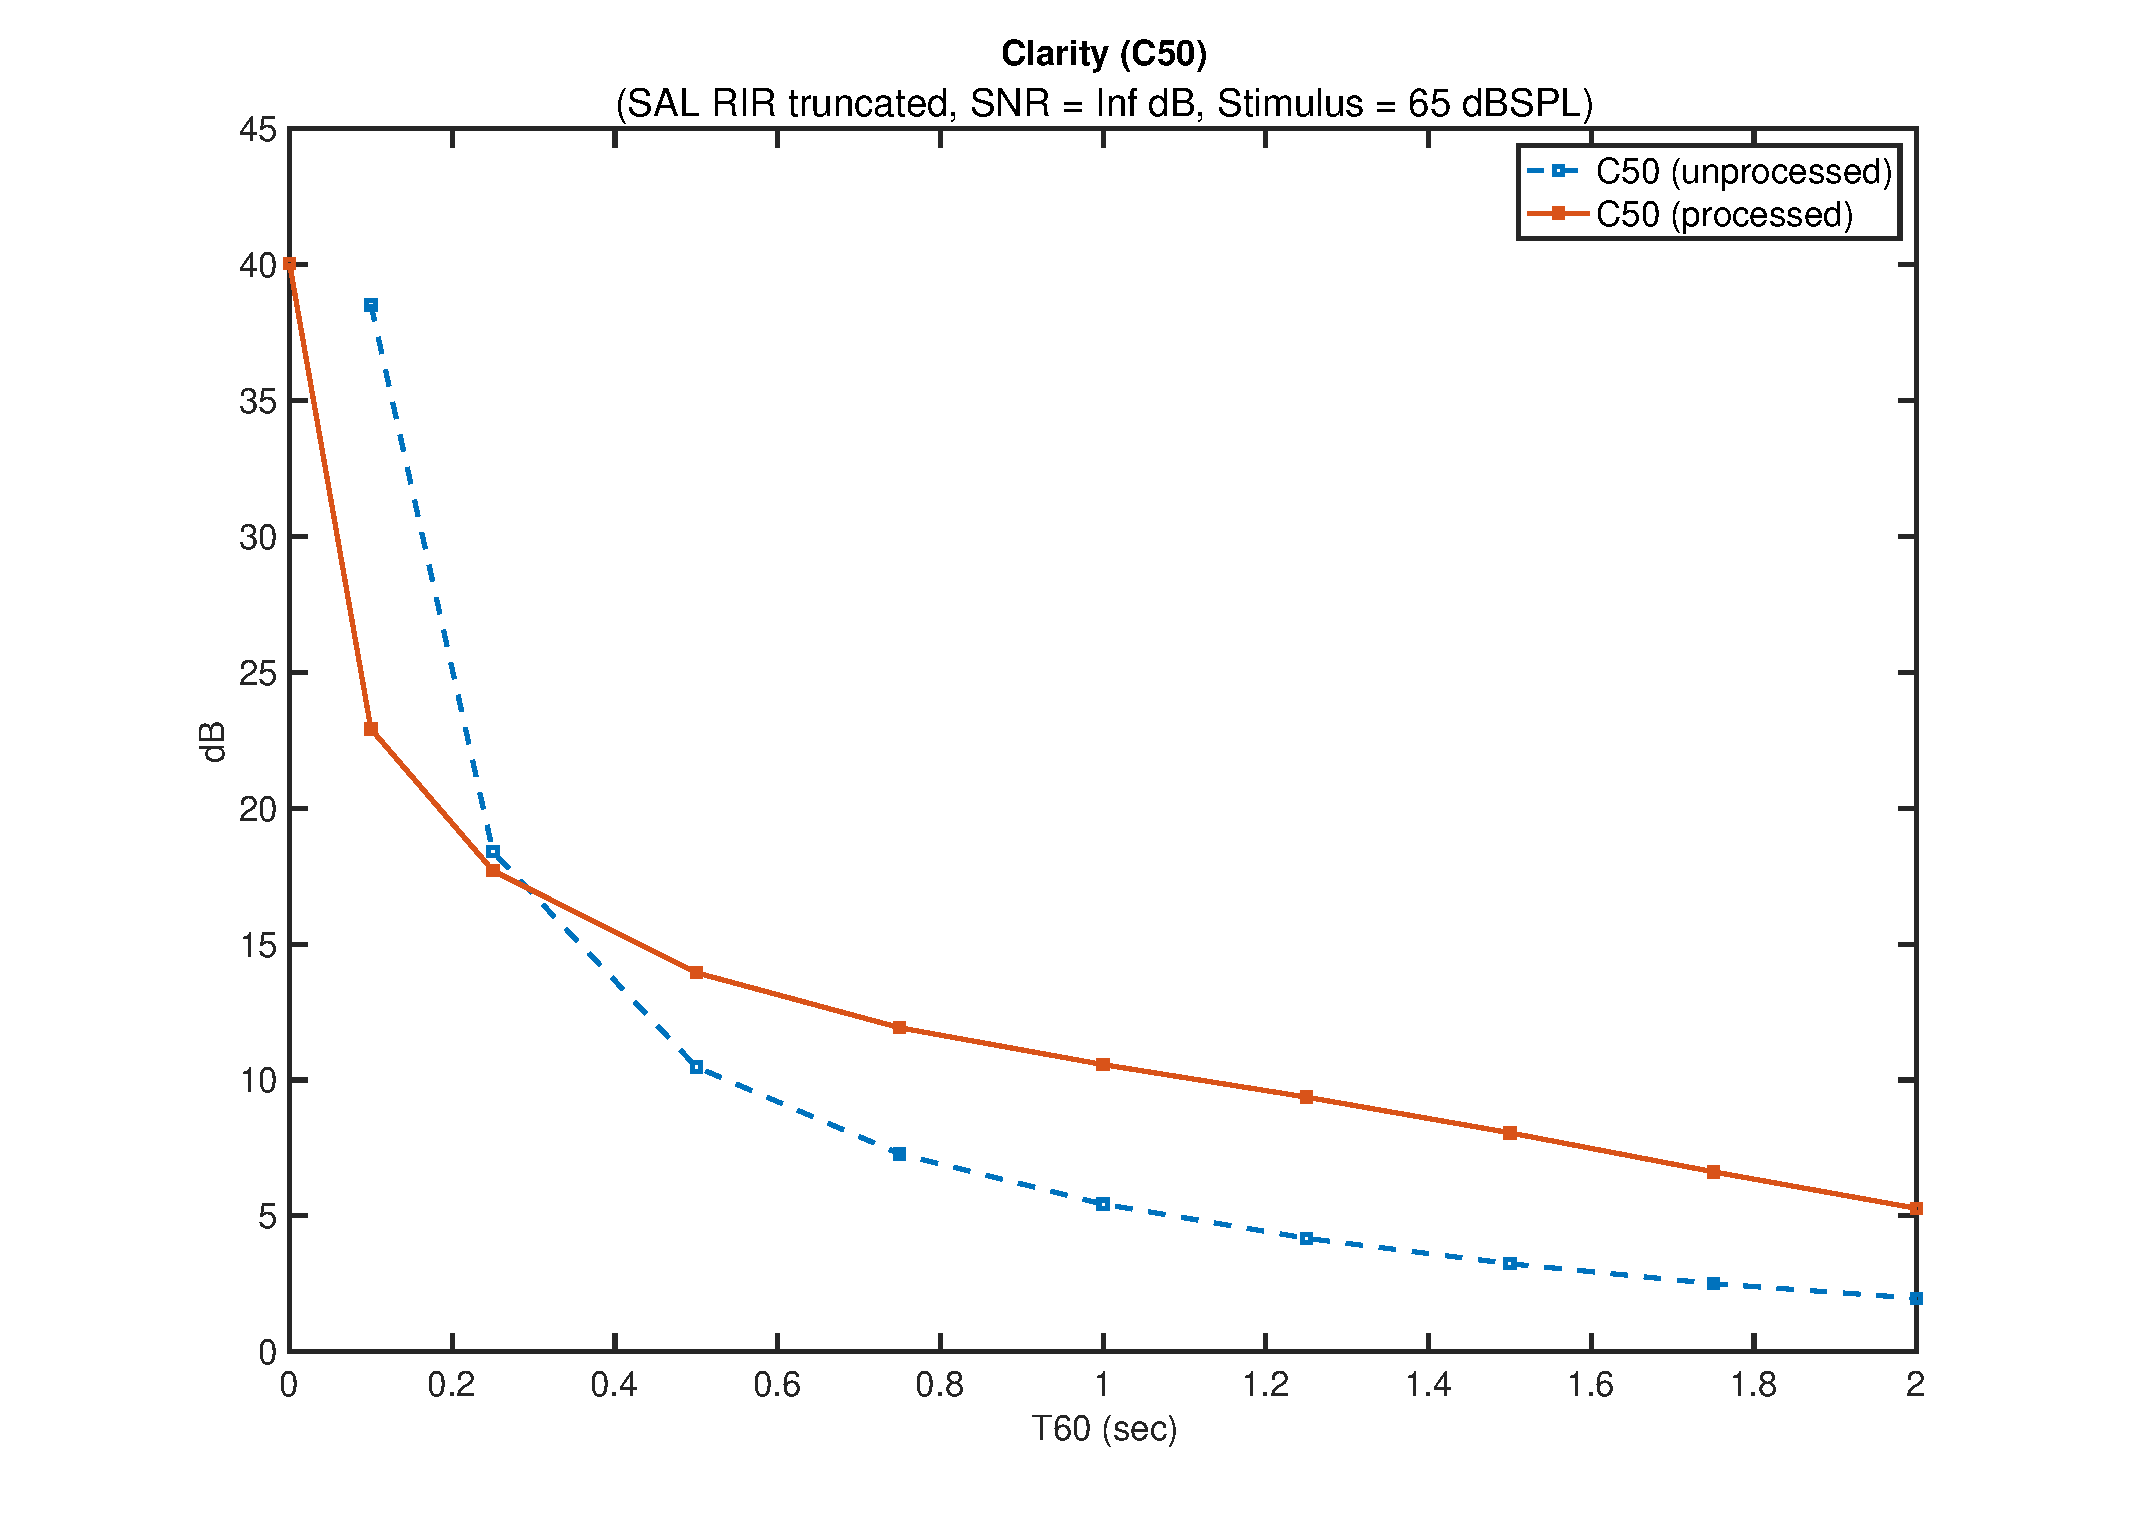
\includegraphics[width=\textwidth]{DAP_EvalT60Sweep_TruncatedSAL_NoNoise_C50_v_T60}
	\end{subfigure}
	\begin{subfigure}[b]{0.92\textwidth}
		\centering
		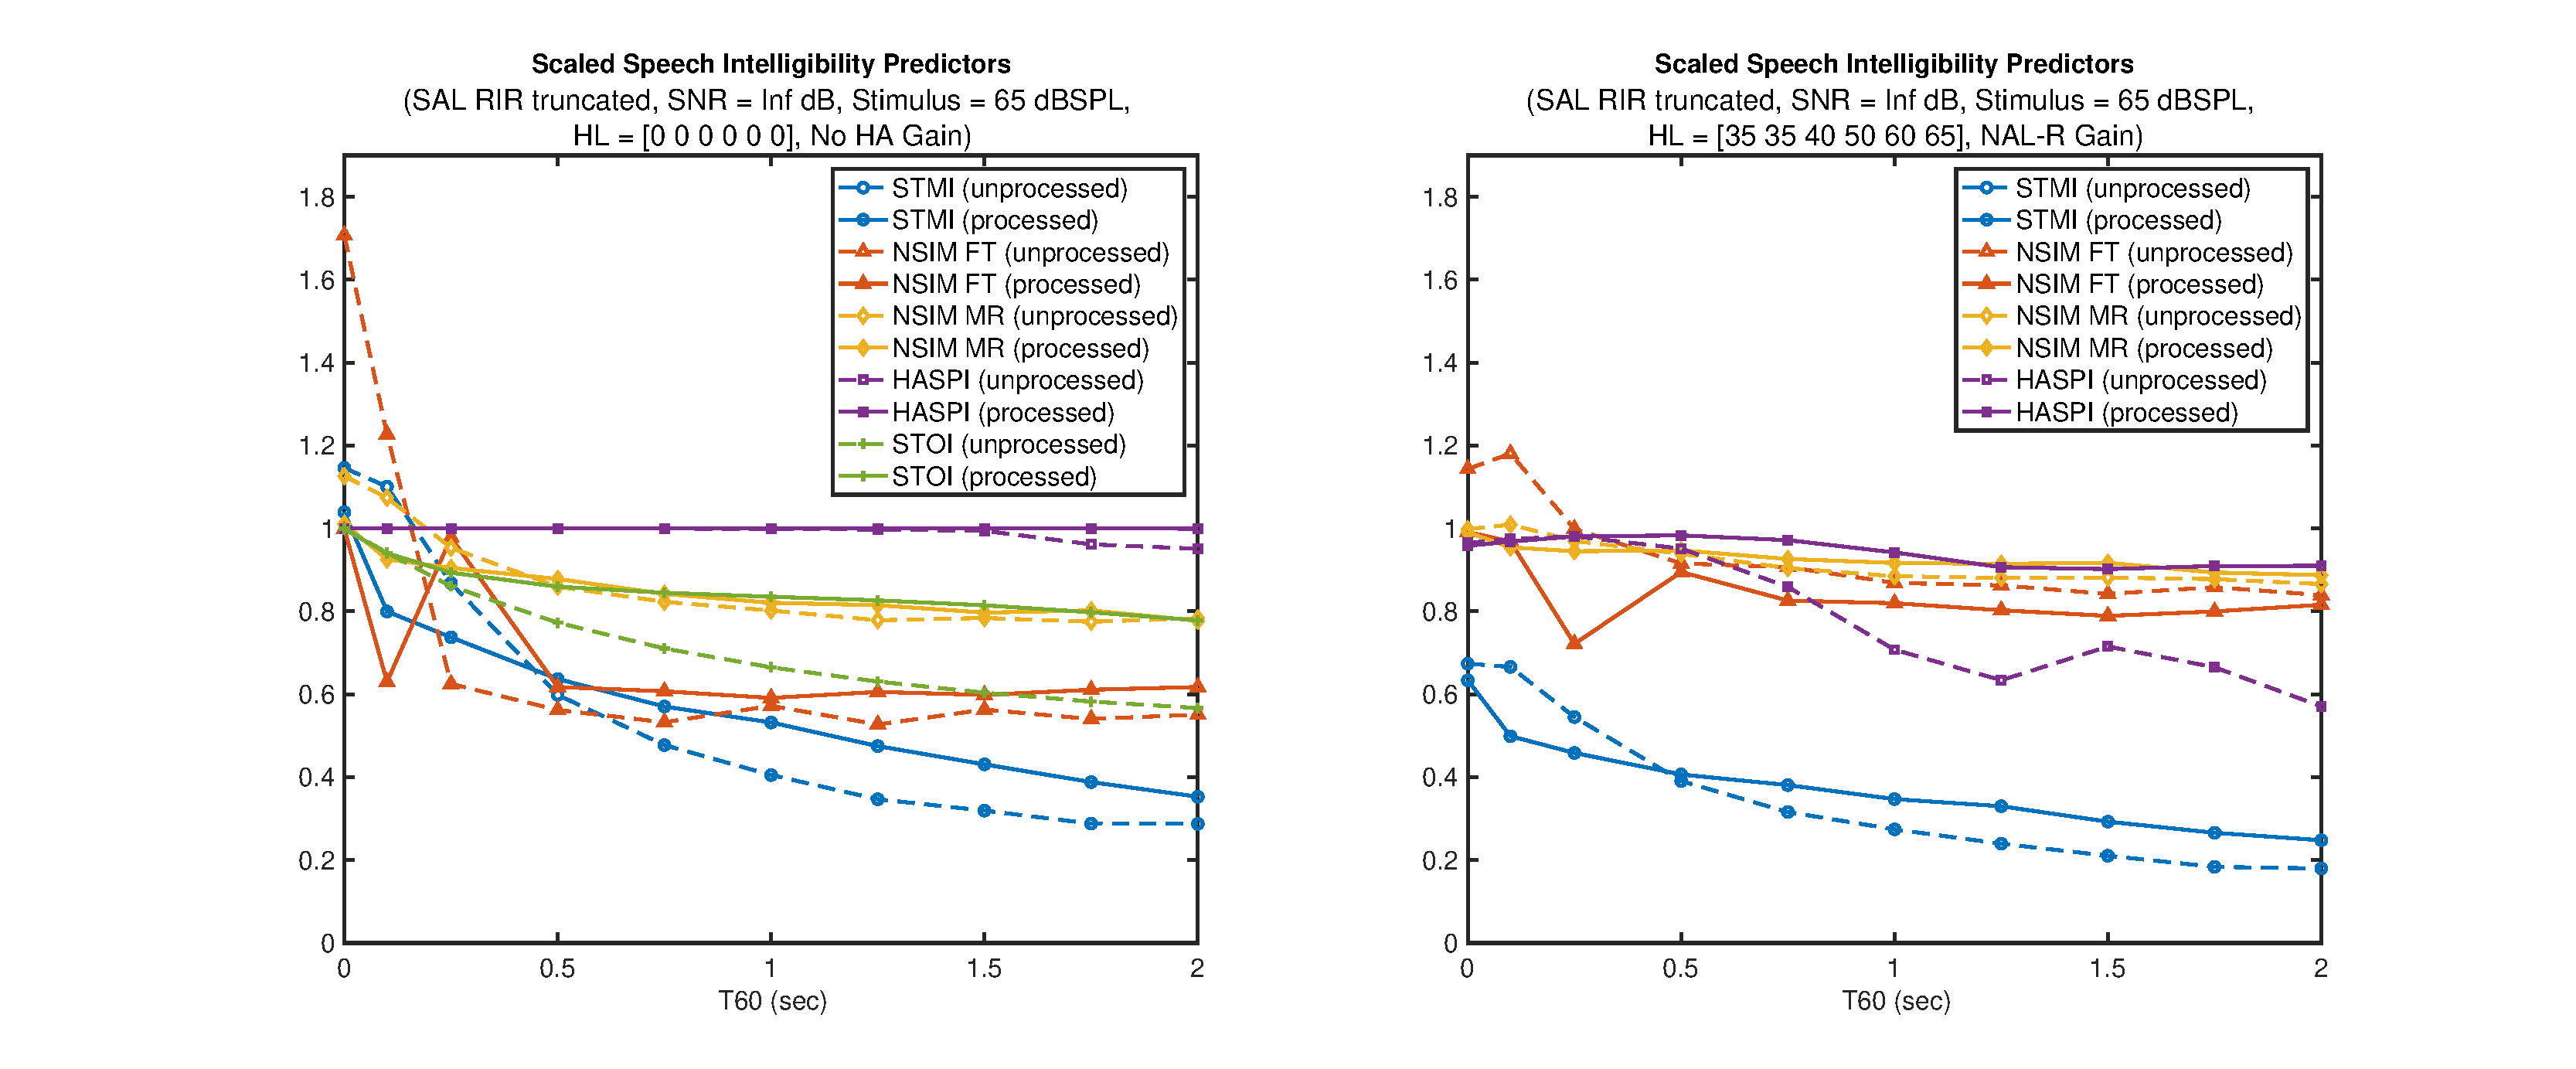
\includegraphics[width=\textwidth]{DAP_EvalT60Sweep_TruncatedSAL_NoNoise_SI_v_T60}
	\end{subfigure}
	\begin{subfigure}[b]{0.92\textwidth}
		\centering
		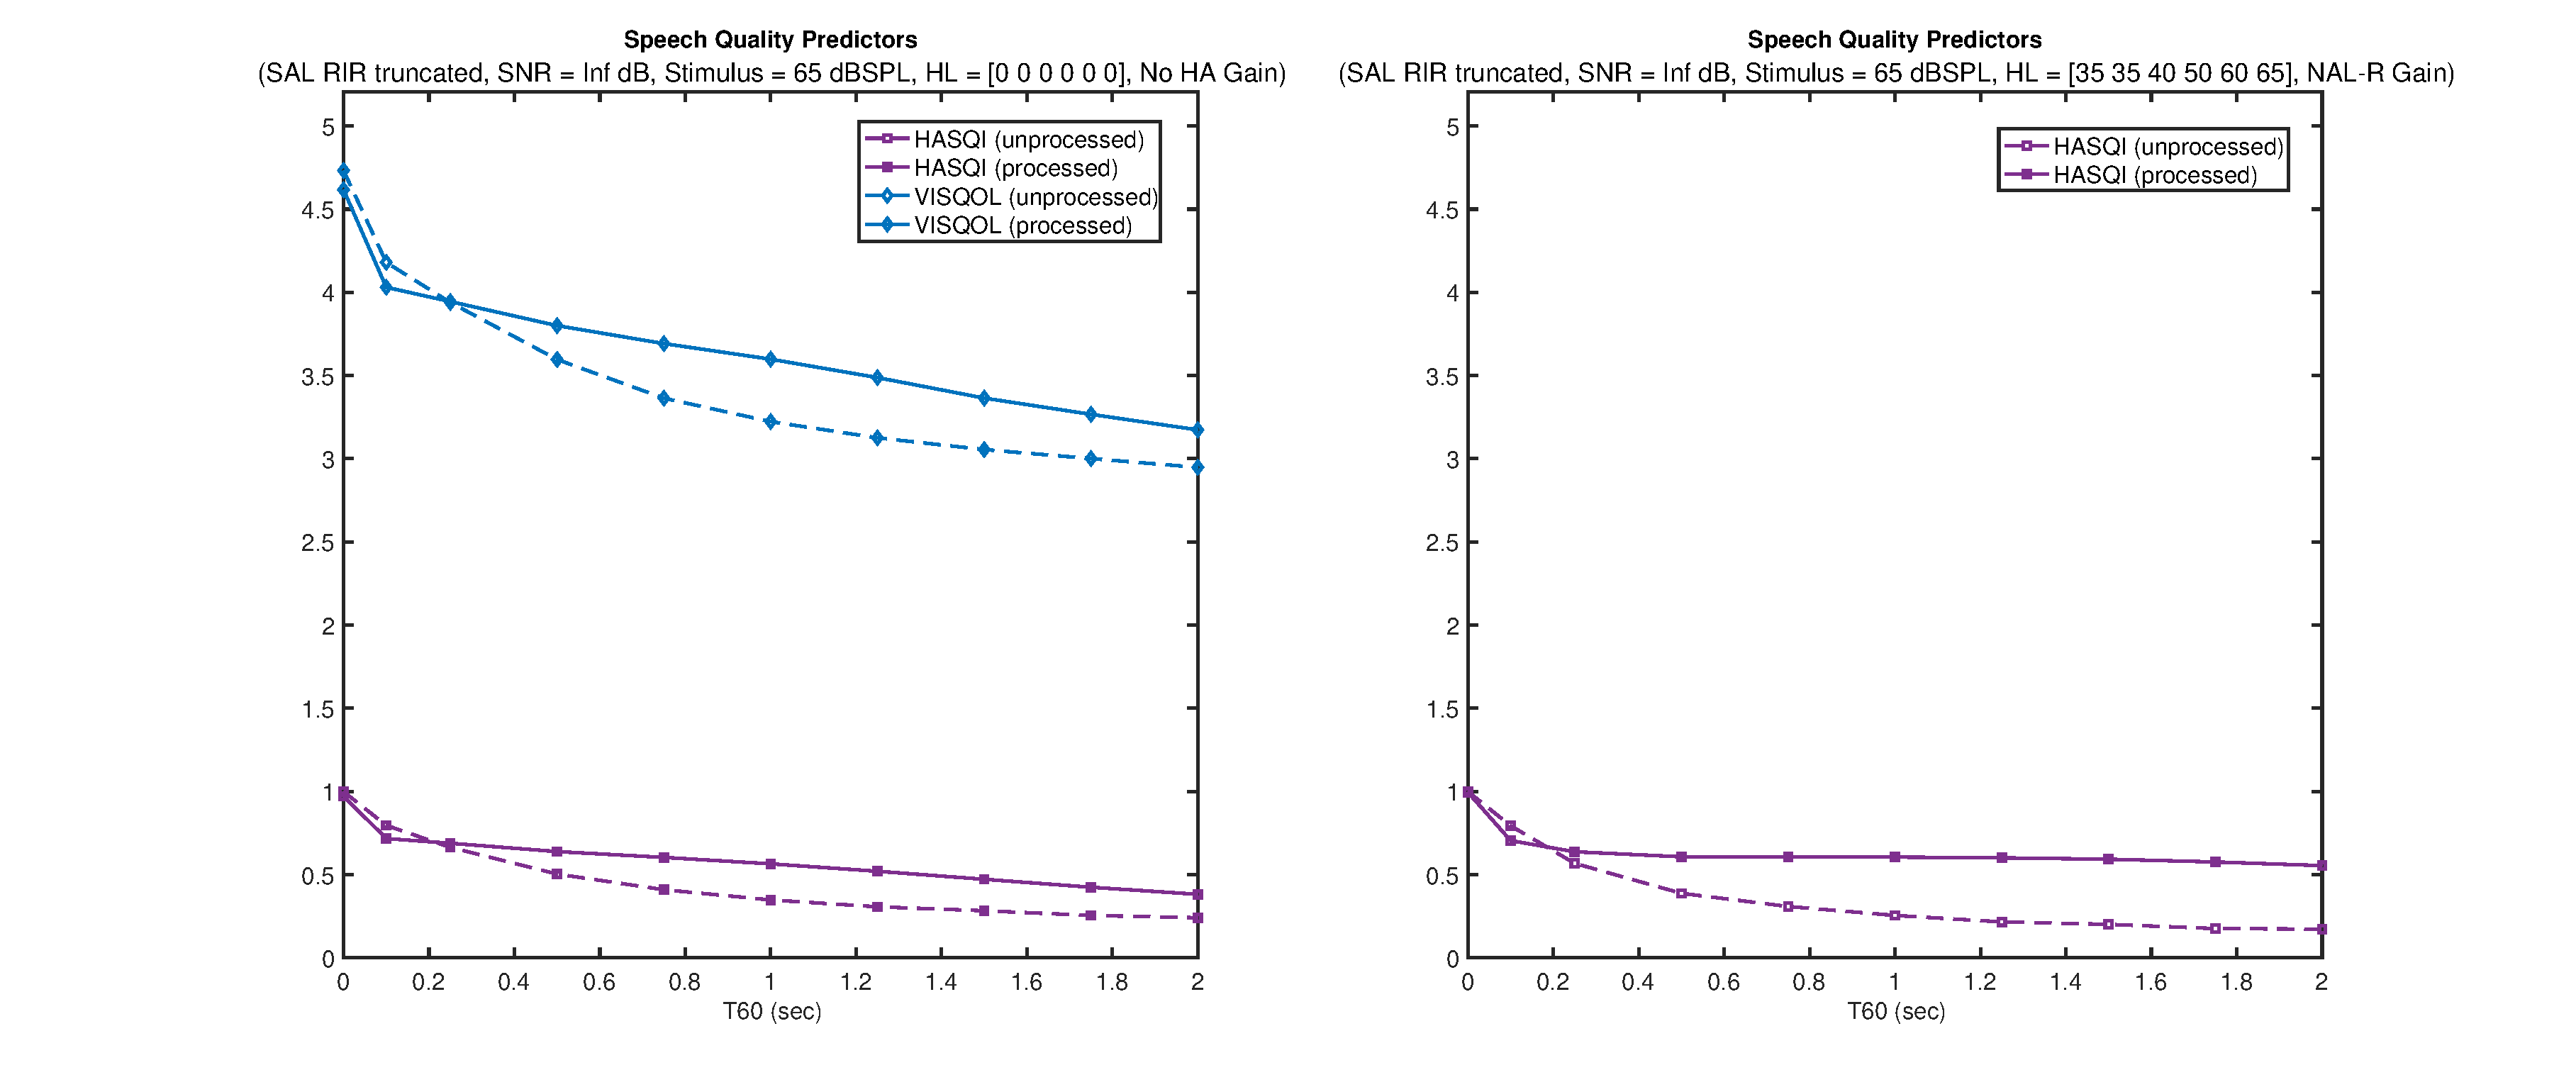
\includegraphics[width=\textwidth]{DAP_EvalT60Sweep_TruncatedSAL_NoNoise_SQ_v_T60}
	\end{subfigure}
	\caption{Evaluation of delay-and-predict dereverberation performance as a function of T60. RIRs were generated by applying a variable decay-rate exponential window to a measured RIR (The SAL room from the MYRiAD database, T60 = 2.2 sec) to control T60.}
	\label{fig:DAP_EvalT60Sweep_TruncatedSAL_NoNoise}
\end{figure}


\section{Impact of Noise on Performance}

\textbf{NOTE: metrics computed on dereverberated speech with noise removed to  neglect the impact of noise on perception (only looking at impacts of reverberation)}

\textbf{SI/SQ/Clarity v T60 w/ SNR = [0 or 12] dB depending on whats needed to show cost}


\begin{figure}[H]
	\centering
	\begin{subfigure}[b]{0.47\textwidth}
		\centering
		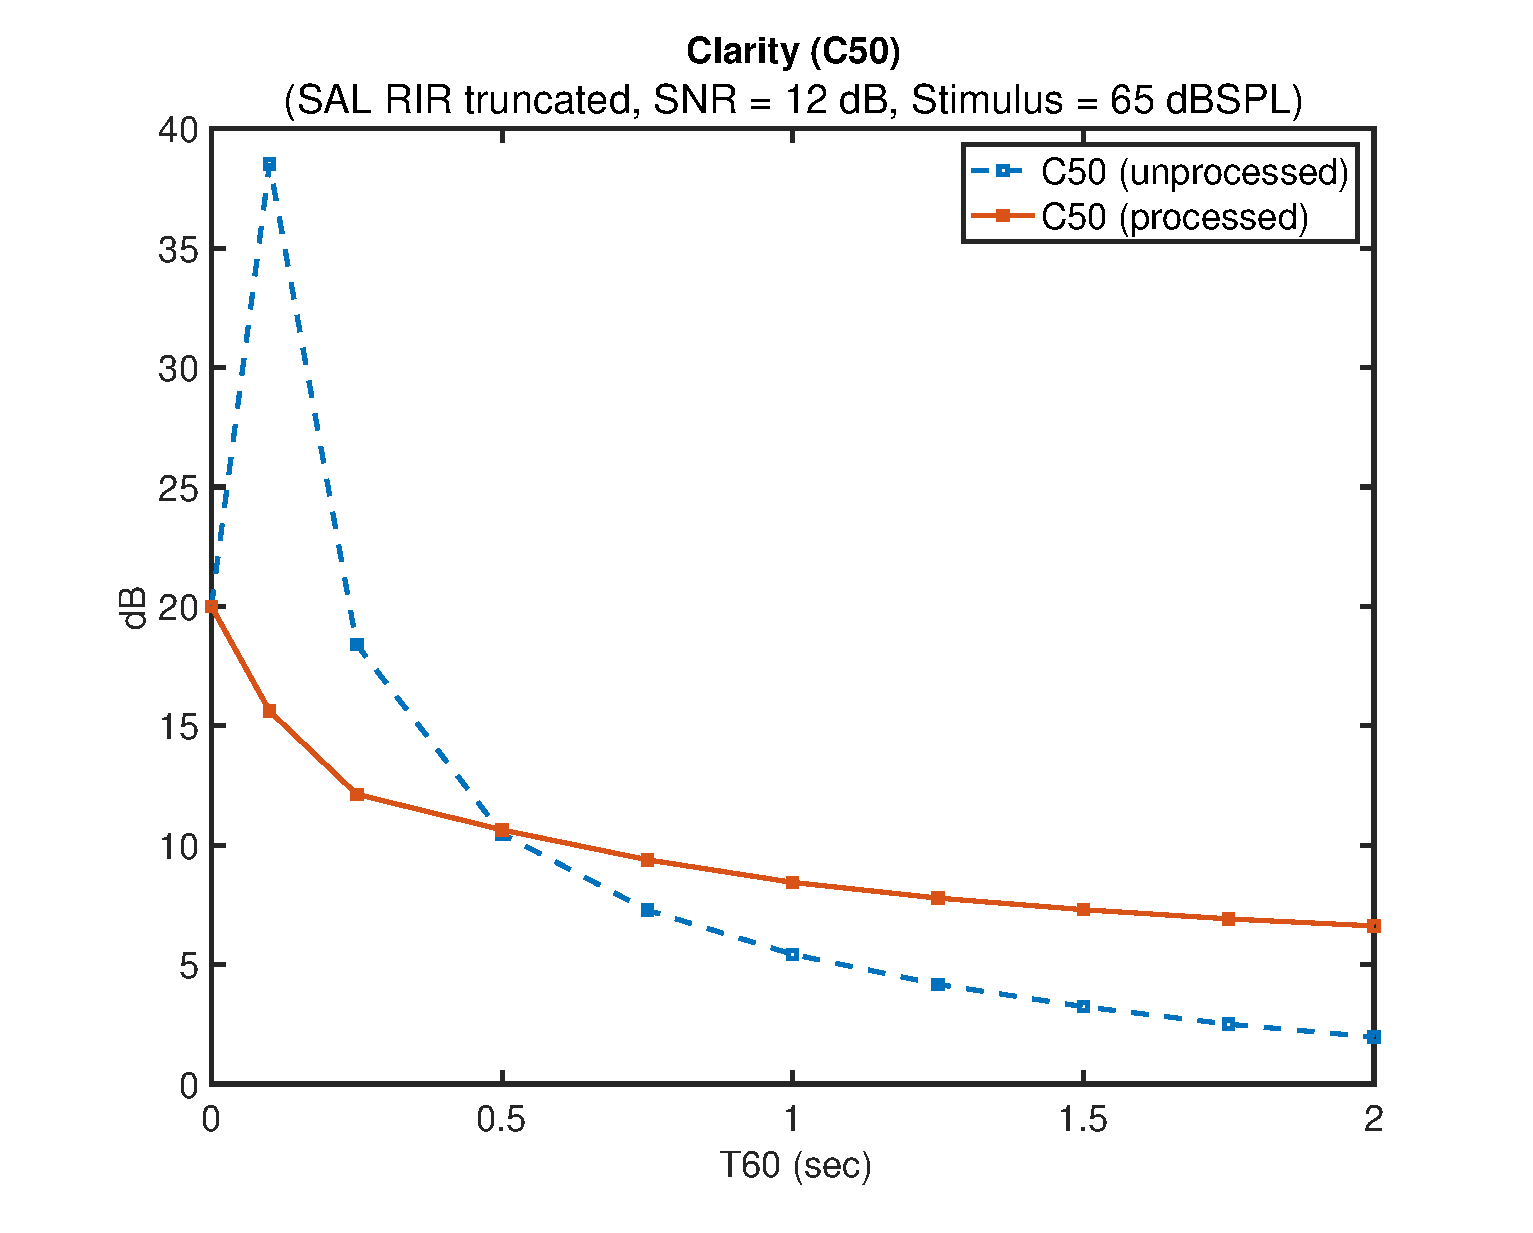
\includegraphics[width=\textwidth]{DAP_EvalT60Sweep_TruncatedSAL_SNR12dB_C50_v_T60}
	\end{subfigure}
	\begin{subfigure}[b]{0.92\textwidth}
		\centering
		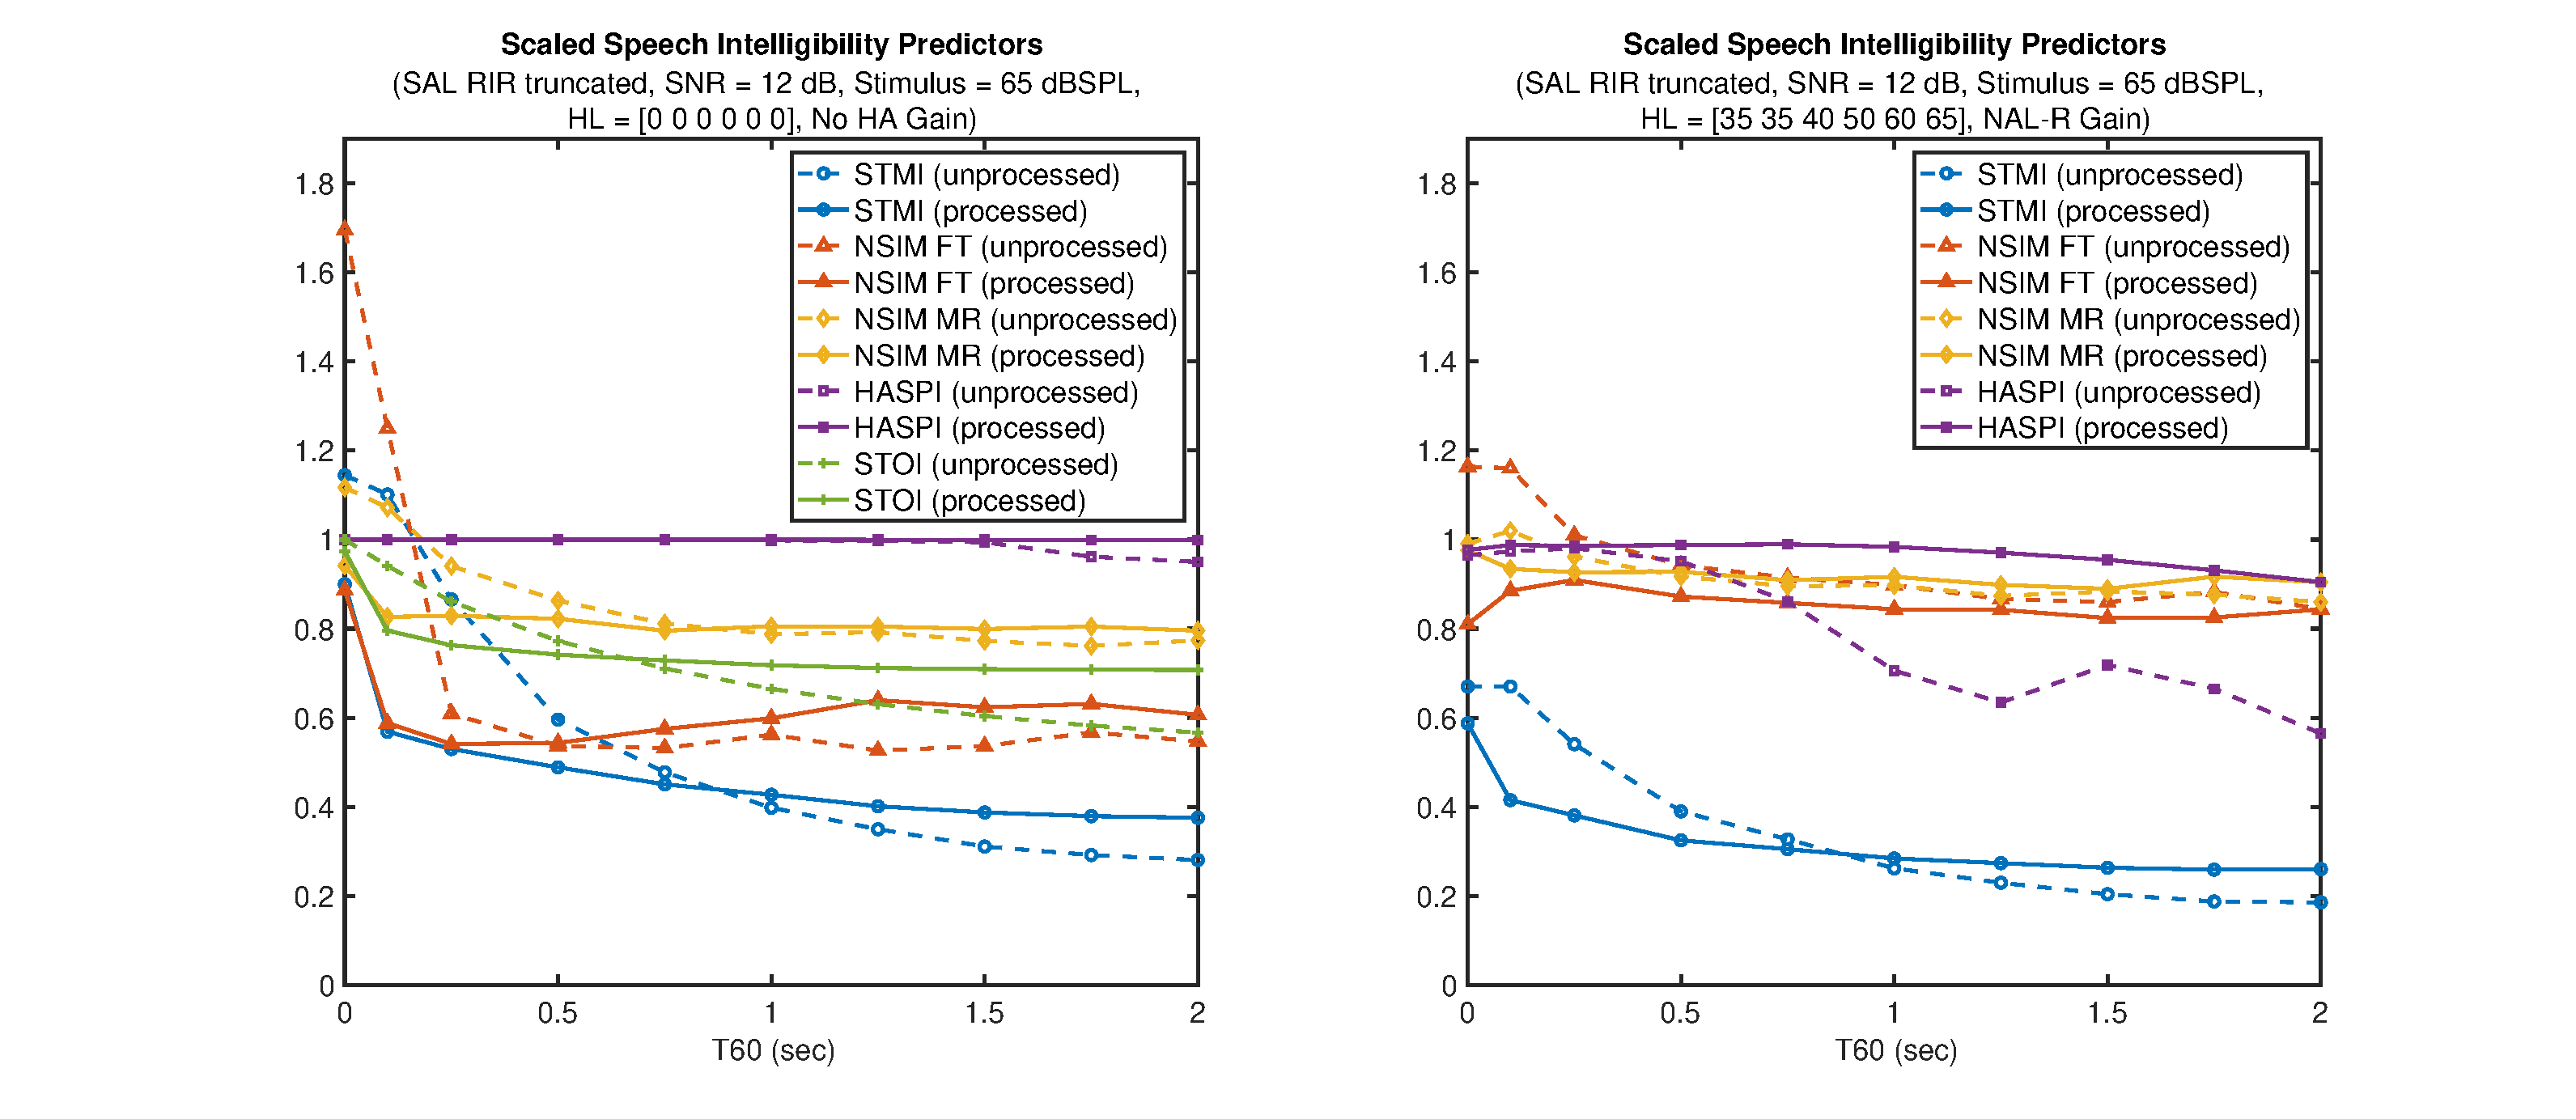
\includegraphics[width=\textwidth]{DAP_EvalT60Sweep_TruncatedSAL_SNR12dB_SI_v_T60}
	\end{subfigure}
	\begin{subfigure}[b]{0.92\textwidth}
		\centering
		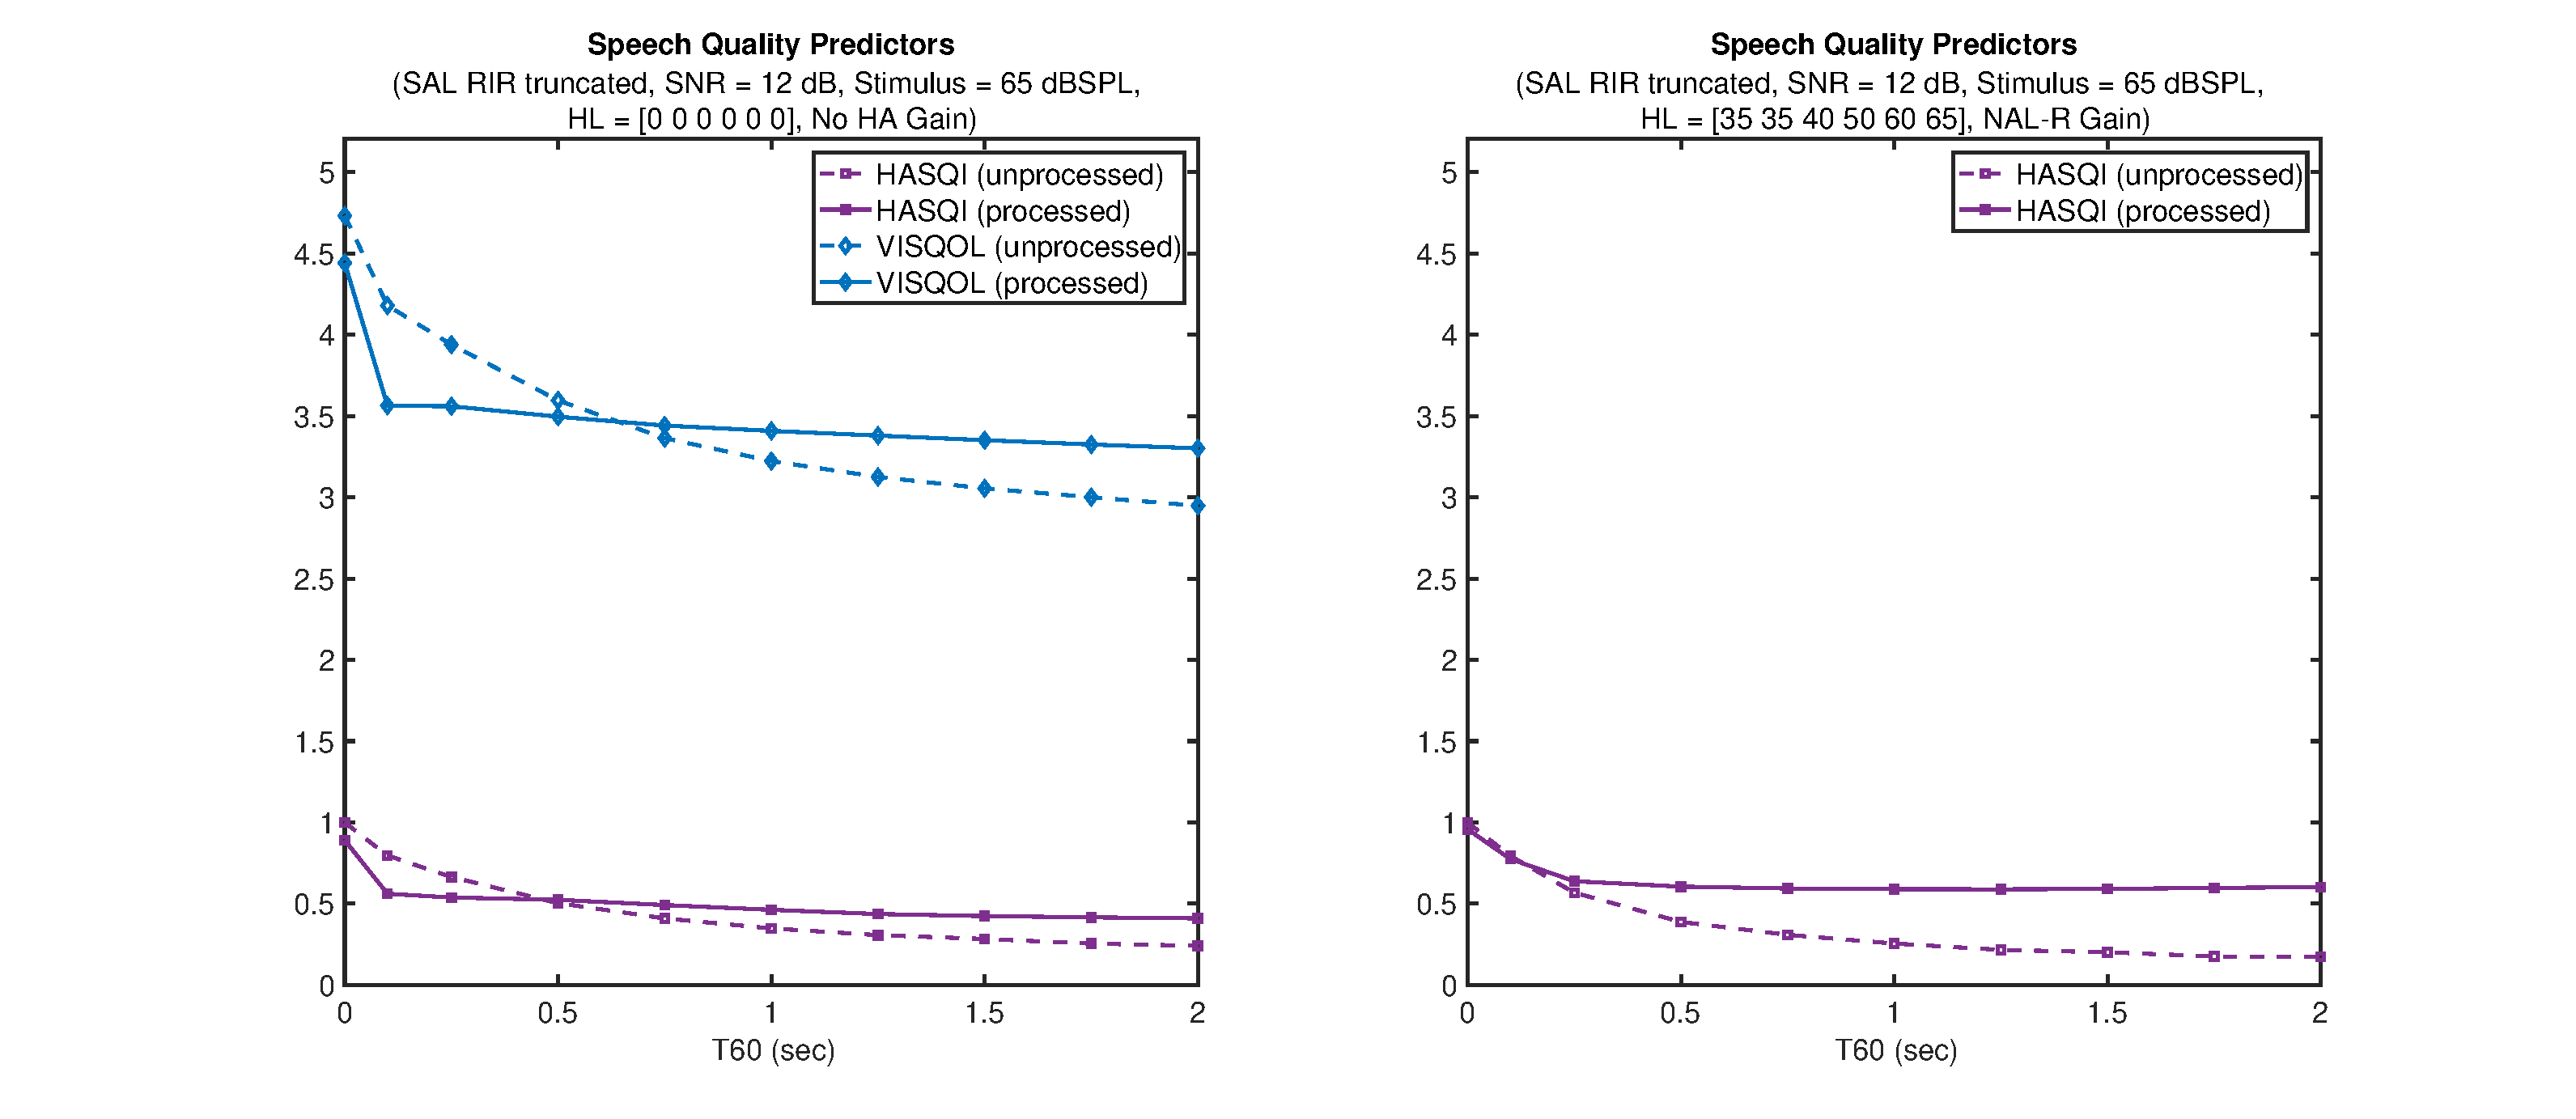
\includegraphics[width=\textwidth]{DAP_EvalT60Sweep_TruncatedSAL_SNR12dB_SQ_v_T60}
	\end{subfigure}
	\caption{Evaluation of delay-and-predict dereverberation performance in the presence of noise as a function of T60. RIRs were generated by applying a variable decay-rate exponential window to a measured RIR (The SAL room from the MYRiAD database, T60 = 2.2 sec) to control T60. Noise was a multichannel recording of approximately stationary noise (Office ventillation noise from the HRIR database), and SNR was set to 12 dB.}
	\label{fig:DAP_EvalT60Sweep_TruncatedSAL_SNR12dB}
\end{figure}

\textbf{SI/SQ/Clarity v SNR w/ T60 = 1 second, stationary noise}

\begin{figure}[H]
	\centering
	\begin{subfigure}[b]{0.47\textwidth}
		\centering
		\includegraphics[width=\textwidth]{DAP_EvalSNRSweepStationary_TruncatedSAL_1000T60_C50_v_SNR}
	\end{subfigure}
	\begin{subfigure}[b]{0.92\textwidth}
		\centering
		\includegraphics[width=\textwidth]{DAP_EvalSNRSweepStationary_TruncatedSAL_1000T60_SI_v_SNR}
	\end{subfigure}
	\begin{subfigure}[b]{0.92\textwidth}
		\centering
		\includegraphics[width=\textwidth]{DAP_EvalSNRSweepStationary_TruncatedSAL_1000T60_SQ_v_SNR}
	\end{subfigure}
	\caption{Evaluation of delay-and-predict dereverberation performance in the presence of noise as a function of SNR. RIRs were generated by applying a variable decay-rate exponential window to a measured RIR (The SAL room from the MYRiAD database, T60 = 2.2 sec) to set T60 = 1 second. Noise was a multichannel recording of approximately stationary noise (Office ventillation noise from the HRIR database).}
	\label{fig:DAP_EvalSNRSweepStationary_TruncatedSAL_1000T60}
\end{figure}

\textbf{SI/SQ/Clarity v SNR w/ T60 = 1 second, Non-Stationary noise}

\begin{figure}[H]
	\centering
	\begin{subfigure}[b]{0.47\textwidth}
		\centering
		\includegraphics[width=\textwidth]{DAP_EvalSNRSweepNonStationary_TruncatedSAL_1000T60_C50_v_SNR}
	\end{subfigure}
	\begin{subfigure}[b]{0.92\textwidth}
		\centering
		\includegraphics[width=\textwidth]{DAP_EvalSNRSweepNonStationary_TruncatedSAL_1000T60_SI_v_SNR}
	\end{subfigure}
	\begin{subfigure}[b]{0.92\textwidth}
		\centering
		\includegraphics[width=\textwidth]{DAP_EvalSNRSweepNonStationary_TruncatedSAL_1000T60_SQ_v_SNR}
	\end{subfigure}
	\caption{Evaluation of delay-and-predict dereverberation performance in the presence of noise as a function of SNR. RIRs were generated by applying a variable decay-rate exponential window to a measured RIR (The SAL room from the MYRiAD database, T60 = 2.2 sec) to set T60 = 1 second. Noise was a multichannel recording of non-stationary noise (Cafeteria babble noise from the HRIR database).}
	\label{fig:DAP_EvalSNRSweepNonStationary_TruncatedSAL_1000T60}
\end{figure}
\section{Impact of an Interfering Talker on Performance}

\textbf{NOTE: metrics computed on dereverberated speech with interfering talker removed to  neglect the impact of interfering talker on perception (only looking at impacts of reverberation on primary talker)}

\textbf{SI/SQ/Clarity v T60 w/ SNR = [0 or 12] dB depending on whats needed to show cost}


\begin{figure}[H]
	\centering
	\begin{subfigure}[b]{0.47\textwidth}
		\centering
		\includegraphics[width=\textwidth]{DAP_EvalT60Sweep_TruncatedSAL_SIR12dB_C50_v_T60}
	\end{subfigure}
	\begin{subfigure}[b]{0.92\textwidth}
		\centering
		\includegraphics[width=\textwidth]{DAP_EvalT60Sweep_TruncatedSAL_SIR12dB_SI_v_T60}
	\end{subfigure}
	\begin{subfigure}[b]{0.92\textwidth}
		\centering
		\includegraphics[width=\textwidth]{DAP_EvalT60Sweep_TruncatedSAL_SIR12dB_SQ_v_T60}
	\end{subfigure}
	\caption{Evaluation of delay-and-predict dereverberation performance in the presence of an interfering talker, as a function of T60. RIRs were generated by applying a variable decay-rate exponential window to a measured RIR (The SAL room from the MYRiAD database, T60 = 2.2 sec) to control T60. Similarly, a measured RIR from a different location in the room was exponentially windowed and used for the interfering talker. The primary-to-interfering talker ratio, i.e., signal-to-interference ratio, was set to SIR = 12 dB.}
	\label{fig:DAP_EvalT60Sweep_TruncatedSAL_SIR12dB}
\end{figure}


